
\documentclass{llncs}

\pagestyle{plain}

% Estos son los paquetes q ocupan todas las versiones del paper (normal y eprint)
\usepackage{setspace}
\usepackage{amsmath,amsfonts,amssymb,amstext}
\usepackage{mathtools}
\usepackage{latexsym,ifthen}
\usepackage{bbm,url}
\usepackage{float}
%\usepackage{bbold}
%\usepackage{amsthm}
\usepackage{bm}
\usepackage{xspace}
%\usepackage[pdftex,usenames,dvipsnames]{color}
\usepackage[usenames,dvipsnames]{color}
%\newtheorem{theorem}{Theoremh}
% \newtheorem{lemma}[theorem]{Lemma}
%\newtheorem{definition}{Definition}
%\newtheorem{example}{Example}
%\newtheorem{remark}{Remark}
%\usepackage{fullpage}
%\usepackage[margin=1.1in]{geometry}
\usepackage{tikz}
\usepackage{xspace}
\usetikzlibrary{arrows,chains,matrix,positioning,scopes,patterns}
\usepackage{authblk}
\usepackage[pdftex,pagebackref]{hyperref}
\usepackage{multirow}
\usepackage{wasysym}
%\usepackage{enumitem}
\usepackage[font=scriptsize]{caption}

% Temporal
\usepackage{soul}

%\usepackage[inline]{enumitem}
\usepackage{enumerate}

\newcommand{\err}{\mathsf{err}}

\newcommand{\cat}{|}
\newcommand{\dsum}{/}
\newcommand{\pdsum}[2]{\mathrm{diag}(#1,#2)}

\newcommand{\sblt}{\stackrel{s}{\bullet}}

\newcommand{\algSize}{normalsize} 
%\newcommand{\algSize}{footnotesize}
\newcommand{\sfleft}{{\mathsf{left}}}
\newcommand{\sfright}{{\mathsf{right}}}

\newcommand{\ps}{\Psi({\dist_k})}
\newcommand{\psws}{{\Psi(\overline{\dist}_k)}}
\newcommand{\sps}{{\Psi_{\mathsf{spl}}(\dist_k)}}
\newcommand{\Sps}{\Psi_{\mathsf{spl}}}
\newcommand{\spsws}{{\Psi_\mathsf{spl}(\overline{\dist}_k)}}
\newcommand{\Spsws}{\Psi_\mathsf{spl}}
\newcommand{\spsmas}{\Psi_{\sfsum}(\dist_k)}
\newcommand{\Spsmas}{\Psi_{\sfsum}}
\newcommand{\spswsmas}{\Psi_{\sfsum}(\overline{\dist}_k)}
\newcommand{\Spswsmas}{\Psi_{\sfsum}}
\newcommand{\spswscomm}{{\Psi_{\mathsf{com}}(\overline{\dist}_k)}}
\newcommand{\Spswscomm}{\Psi_{\mathsf{com}}}
\newcommand{\bbb}{\bar{b}}
\newcommand{\capprox}{\overset{c}{\approx}}

\newcommand{\latexDeMierdaEstupido}{]}

\newcommand{\Comm}{\mathsf{Comm}}
\newcommand{\Com}{\mathsf{Com}}
\newcommand{\vect}{\mathbf{vec}}

\newcommand{\lef}{{\mathtt{l}}}
\newcommand{\rig}{{\mathtt{r}}}
\newcommand{\stmnt}{\mathsf{stm}}
%Commitment keys

%Log Left Commitment Key
\newcommand{\llck}{\vecb{g}}
%Log Right Commitment Key
\newcommand{\lrck}{\vecb{h}}
%Left Commitment Key
\newcommand{\lck}{[{\llck}]_1}
%Right Commitment Key
\newcommand{\rck}{[{\lrck}]_2}
\newcommand{\rcks}{[{\lrck}]_1}

%Commitement keys matrices

%Log Left Commitment Keys
\newcommand{\Llck}{\matr{G}}
%Log Right Commitment Keys
\newcommand{\Lrck}{\matr{H}}
%Left Commitment Keys
\newcommand{\Lck}{[\Llck]_1}
%Right Commitment Keys
\newcommand{\Rck}{[{\Lrck}]_2}
\newcommand{\Rcks}{[{\Lrck}]_1}

%For quadratic info \lck\rck^\top
\newcommand{\Lqmatr}{\matr{C}}
\newcommand{\Qmatr}{{[\Lqmatr]_1}}
\newcommand{\Qspace}{\mathcal{C}}

% c_\Delta
\newcommand{\lccom}{\vecb{c}_\Delta}
\newcommand{\ccom}{\hvecb{c}_\Delta}

\newcommand{\pke}{\mathsf{PKE}}
\newcommand{\kem}{\mathsf{KEM}}
\newcommand{\prf}{\mathsf{PRF}}
\newcommand{\ev}{\mathsf{F}}
\newcommand{\KEM}{\mathsf{KEM}}
\newcommand{\gen}{\mathsf{Gen}}
\newcommand{\enc}{\mathsf{Enc}}
\newcommand{\Enc}{\mathsf{Enc}}
\newcommand{\dec}{\mathsf{Dec}}
\newcommand{\Dec}{\mathsf{Dec}}
\newcommand{\pk}{\mathit{pk}}
\newcommand{\sk}{\mathit{sk}}
\newcommand{\cdh}{\ensuremath{\mathsf{CDH}}}
\newcommand{\ddh}{\ensuremath{\mathsf{DDH}}}
\newcommand{\sxdh}{\ensuremath{\mathsf{SXDH}}}
\newcommand{\mddh}{\ensuremath{\mathsf{MDDH}}}
\newcommand{\mcdh}{\ensuremath{\mathsf{MCDH}}}
\newcommand{\fmdh}{\ensuremath{\mathsf{KerMDH}}}
\newcommand{\bddh}{\ensuremath{\mathsf{BDDH}}}
\newcommand{\mat}[1]{\ensuremath{#1\mbox{-}\mathsf{Mat}}}
\newcommand{\pddh}[1]{\ensuremath{#1\mbox{-}\mathsf{PDDH}}}
\newcommand{\mlddh}[1]{\ensuremath{#1\mbox{-}\mathsf{MLDDH}}}
\newcommand{\eddh}[1]{\ensuremath{#1\mbox{-}\mathsf{EDDH}}}
\newcommand{\casc}[1]{\ensuremath{#1\mbox{-}\mathsf{Casc}}}
\newcommand{\scasc}[1]{\ensuremath{#1\mbox{-}\mathsf{SCasc}}}
\newcommand{\lin}[1]{\ensuremath{#1\mbox{-}\mathsf{Lin}}}
\newcommand{\rlin}[1]{\ensuremath{#1\mbox{-}\mathsf{RLin}}}
\newcommand{\re}{\mathsf{RE}_\G}
\newcommand{\kcirc}[1]{\ensuremath{#1\mbox{-}\mathsf{Circ}}}
\newcommand{\escQE}{\gamma}
\newcommand{\EscQE}{\Gamma}


% M \in Z^{\la \times \lb}, N\in Z^{\la \times \lc}, \Lambda\in Z^{\ld\times \lb}
% x \in \Z_q^\la, b\in \Z_q^\lb, w\in\Z_q^\lc, \alpha\in \Z_q^\ld
\newcommand{\la}{{\ell_1}}
\newcommand{\lb}{{m}}
\newcommand{\lc}{{\ell_2}}
\newcommand{\ld}{{\ell_3}}


\newcommand{\LangMN}{{\Lang_{[\matr{M}]_1,[\matr{N}]_1,\matr{\Lambda},\grkb{\alpha}}}}



\newcommand{\skermdh}{\ensuremath{\mathsf{SKerMDH}}}
\newcommand{\kermdh}{\ensuremath{\mathsf{KerMDH}}}
\newcommand{\akermdh}{\ensuremath{\mathsf{aKerMDH}}}

\newcommand{\KG}{\mathsf{KeyGen}}
\newcommand{\GS}{{\mathsf{GS}}}

%HPS definitions
\newcommand{\univo}{universal$_1$\xspace}
\newcommand{\univt}{universal$_2$\xspace}
\newcommand{\distance}[2]{\Delta\left[#1 \,,\, #2\right]}
\newcommand{\entropic}{entropic\xspace}
\newcommand{\ciphertext}{{c}}
\def\params{\mathit{params}}
\newcommand{\structure}{\mathcal{S}}
\newcommand{\ciphersp}{\mathcal{C}}
\newcommand{\conssp}{\mathcal{V}}
\newcommand{\primeorder}{p}
\newcommand{\keysp}{\mathcal{K}}
\def\hps{\varfont{hps}}
\newcommand{\advBhps}{\calB}
\newcommand{\advBhpso}{\calB_{1}}
\newcommand{\advBhpst}{\calB_{2}}
\newcommand{\PK}{\mathcal{PK}}
\newcommand{\SK}{\mathcal{SK}}
\newcommand{\hash}{\mu}
\newcommand{\bigiota}{\mathcal{I}}
\newcommand{\var}[1]{{\mathsf{#1}}}
\newcommand{\vvar}[1]{{\mathbf{\var{#1}}}}
\newcommand{\varb}{\mathsf{b}}
\newcommand{\varx}{\mathsf{x}}
\newcommand{\vvarx}{\textbf{\textsf{x}}}
\newcommand{\vary}{\mathsf{y}}
\newcommand{\vvary}{\textbf{\textsf{y}}}
\newcommand{\varz}{\mathsf{z}}
\newcommand{\varX}{\mathsf{X}}
\newcommand{\varY}{\mathsf{Y}}
\newcommand{\varZ}{\mathsf{Z}}
\newcommand{\varvecx}{\vec{\varx}}
\newcommand{\varvecy}{\vec{\vary}}
\newcommand{\varvecz}{\vec{\varx}}
\newcommand{\hcx}{(\hat{x}_1,\ldots,\hat{x}_m)}
\newcommand{\matrB}{\matr{B}} 
\newcommand{\vecL}{(\hat{l}_1,\ldots,\hat{l}_n)}



% Las instancias de SPLHS se van a llamr \Phi
\newcommand{\SPLHSinst}{\Phi}
\newcommand{\SG}{\mathsf{SignGen}}
\newcommand{\SN}{\mathsf{Sign}}
\newcommand{\SD}{\mathsf{SignDerive}}
\newcommand{\SV}{\mathsf{Verify}}
\newcommand{\SP}{\ensuremath{\mathsf{SP}}}
\newcommand{\poly}{\mathsf{poly}}

%Comicmens a los eltos de la listas
\newcommand{\lcom}{\vecb{f}}
\newcommand{\Lcom}{\matr{F}}

%Definition
\newcommand{\MP}{\mathsf{MP}}
\newcommand{\GScom}{\mathsf{GS.Com_{\hvecb{U}}}}
\newcommand{\MPcomg}{\mathsf{MP.Com}_{\hmatr{G}}}
\newcommand{\MPcomh}{\mathsf{MP.Com}_{\hmatr{H}}}




% QA-NIZK for linear spaces
\newcommand{\ZKLinInst}{\mathsf{ZKLin}}
\newcommand{\ZKLinK}{\mathsf{ZKLin.K}_0}
\newcommand{\ZKLinKK}{\mathsf{ZKLin.K}_1}
\newcommand{\ZKLinCRS}{\mathsf{ZKLin.crs}}

\newcommand{\QANIZKsum}{{\spswsmas}}
\newcommand{\QANIZKcomms}{{\spswscomm}}
\newcommand{\QANIZKsym}{{\Psi_{\mathsf{sym}}}}

\newcommand{\nb}{{\overline{n}}}

\newcommand{\bb}{\overline{b}}
\newcommand{\bub}{{b(\overline{b}-1)}}
\newcommand{\tm}{\tilde{m}}

\newcommand{\rank}{\mathbf{rank}}
\newcommand{\HPSscheme}{\mathsf{HPS}}
%\newcommand{\THPSscheme}{\schemefont{HPS_t}}
% \newcommand{\THPSscheme}{\mathsf{HPS^{td}}}
% \newcommand{\HHPSscheme}{\mathsf{HPS}_2}
\newcommand{\HPSsys}{\mathsf{Param}}
\newcommand{\HPSpub}{\mathsf{Pub}}
\newcommand{\HPSpriv}{\mathsf{Priv}}
\newcommand{\HPSdec}{\mathsf{Decide}}
\newcommand{\eval}{\Lambda}
%\newcommand{\hpscu}{{\notionfont{cu}_2}}
%\newcommand{\ExpHPScu}[2]{\Exp^{\hpscu}_{#1,#2}}
%\newcommand{\AdvHPScu}[2]{\Adv^{\hpscu}_{#1,#2}}
%\newcommand{\hpscub}{{\notionfont{\hpscu\mbox{-}b}}}
%\newcommand{\hpscuz}{{\notionfont{\hpscu\mbox{-}0}}}
%\newcommand{\hpscuo}{{\notionfont{\hpscu\mbox{-}1}}}
%\newcommand{\ExpHPScub}[2]{\Exp^{\hpscub}_{#1,#2}}
%\newcommand{\ExpHPScuo}[2]{\Exp^{\hpscuo}_{#1,#2}}
%\newcommand{\ExpHPScuz}[2]{\Exp^{\hpscuz}_{#1,#2}}
% \newcommand{\pcol}{\delta}
\newcommand{\prcol}{\delta}
\newcommand{\trapdoor}{\omega}
\newcommand{\witness}{r}
\newcommand{\algD}{\mathsf{D}}
\newcommand{\algK}{\mathsf{K}}
\newcommand{\algG}{\mathsf{G}}
\newcommand{\algP}{\mathsf{P}}
\newcommand{\algV}{\mathsf{V}}
\newcommand{\algS}{\mathsf{S}}
\newcommand{\algF}{\mathsf{F}}
\newcommand{\algVrfy}{\mathsf{Vrfy}}

\newcommand{\R}{\mathcal{R}}
\newcommand{\M}{\mathcal{M}}
\newcommand{\dist}{\mathcal{D}}
\newcommand{\distw}{\mathcal{W}}
\newcommand{\distk}{\mathcal{K}}
\newcommand{\distlin}{\mathcal{L}}
\newcommand{\distrlin}{\mathcal{RL}}
\newcommand{\distc}{\mathcal{C}}
\newcommand{\distsc}{\mathcal{SC}}
\newcommand{\distcirc}{\mathcal{CI}}
\newcommand{\distu}{\mathcal{U}}
\newcommand{\distp}{\mathcal{P}}
\newcommand{\distink}{\dist_k^{m,i}}
\newcommand{\distjnk}{\dist_1^{m,i}}

\newcommand{\distinmk}{\dist_k^{mn,i}}
\newcommand{\distzeronmk}{\dist_k^{mn,0}}
\newcommand{\distzeronk}{\dist_k^{m,0}}
\newcommand{\distlininone}{\distlin_1^{m,i}}
\newcommand{\distlinisnone}{\distlin_1^{m,i^*}}
\newcommand{\distlinizeroone}{\distlin_1^{m,0}}
\newcommand{\distlinjsnzero}{\distlin_1^{n,j^*}}
\newcommand{\block}[1]{
  \underbrace{\begin{matrix}1 & \cdots & 1\end{matrix}}_{#1}
}
%\newcommand{\gets}{\leftarrow}
\newcommand{\Z}{\mathbb{Z}}
\newcommand{\N}{\mathbb{N}}
\newcommand{\G}{\mathsf{Gen}}
\newcommand{\advD}{\mathsf{D}}
\newcommand{\advA}{\mathsf{A}}
\newcommand{\advB}{\mathsf{B}}
\newcommand{\adv}{\mathbf{Adv}}
\newcommand{\group}{{gk}}
\newcommand{\gk}{\group}
\newcommand{\pgroup}{\mathcal{PG}}
\newcommand{\mgroup}[1]{\mathcal{MG}_{#1}}
\newcommand{\ggen}{\mathsf{Gen}}
\newcommand{\pggen}{\mathsf{PGen}}
\newcommand{\mggen}[1]{\mathsf{MGen}_{#1}}
\newcommand{\heading}[1]{\smallskip\noindent{\sc{#1}}}
\newcommand{\vecb}[1]{{\boldsymbol{#1}}}
\newcommand{\vecbt}[1]{\vec{#1}^{\ \top}}
\newcommand{\uvecb}[1]{{\vect({\vecb{#1}})}}
\newcommand{\tvecb}[1]{{\tilde{\vecb{#1}}}}
\newcommand{\tgrkb}[1]{\tilde{\grkb{#1}}}
\newcommand{\ovecb}[1]{{\overline{\vecb{#1}}}}
\newcommand{\Pt}{\mathcal{P}}
\newcommand{\Opt}{\mathcal{O}}
\newcommand{\pt}[1]{\mathcal{#1}}
\newcommand{\stbl}{\ \tilde \bullet \ }
\newcommand{\bilgroup}{\mathcal{PG}}
\newcommand{\matr}[1]{\mathbf{{#1}}}
\newcommand{\vecw}{\vecb{w}}
\newcommand{\vecr}{\vecb{r}}
\newcommand{\vecz}{\vecb{z}}
\newcommand{\vecy}{\vecb{y}}
\newcommand{\vecx}{\vecb{x}}
\newcommand{\veca}{\vecb{a}}
\newcommand{\matrA}{\matr{A}}
\newcommand{\hmatrA}{\hmatr{A}}
\newcommand{\cmatrA}{\cmatr{A}}
\newcommand{\smallpmatrix}[1]{\left(\begin{smallmatrix}#1\end{smallmatrix}\right)}
\newcommand{\pmatri}[1]{\left(\begin{matrix}#1\end{matrix}\right)}
\newcommand{\bmatri}[1]{\left[\begin{matrix}#1\end{matrix}\right]}
\newcommand{\matri}[1]{{\begin{matrix}#1\end{matrix}}}
\newcommand{\smatri}[1]{{\begin{smallmatrix}#1\end{smallmatrix}}}
\newcommand{\sfsplit}{\mathsf{spl}}
\newcommand{\bulletsp}{ \bullet }
\newcommand{\newf}{\widehat{f}}
\newcommand{\newF}{\widehat{F}}
\newcommand{\com}{\mathsf{com}}
\newcommand{\eq}{\mathsf{eq}}
\newcommand{\eqd}{\equiv}
\newcommand{\negl}{\mathsf{negl}}
\newcommand{\A}{\mathcal{A}}
\newcommand{\GG}{\mathbb{G}}
\newcommand{\ZZ}{\mathbb{Z}}
\newcommand{\Gr}{\ensuremath{\mathbb{G}_1}}
\newcommand{\Hr}{\ensuremath{\mathbb{G}_2}}
\newcommand{\T}{\ensuremath{\mathbb{T}}}
\newcommand{\SSDP}{\ensuremath{\mathsf{SSDP}}}
\newcommand{\PermP}{\ensuremath{\mathsf{PermP}}}
\newcommand{\PP}{\ensuremath{\mathsf{PP^*}}}
\newcommand{\bmatr}[1]{\left[\matr{#1}\right]}
\newcommand{\hmatr}[1]{{\hat{\matr{#1}}}}
\newcommand{\cmatr}[1]{\check{\matr{#1}}}
\newcommand{\bvecb}[1]{\left[\vecb{#1}\right]}
\newcommand{\hvecb}[1]{{\hat{\vecb{#1}}}}
\newcommand{\cvecb}[1]{\check{\vecb{#1}}}
\newcommand{\bits}{\{0,1\}}
\newcommand{\rmIm}{\mathbf{Im}}
\newcommand{\sfGame}{\mathsf{Game}}
\newcommand{\sfReal}{\mathsf{Real}}
\newcommand{\grkb}[1]{{\boldsymbol #1}}
\newcommand{\ugrkb}[1]{{\underline{\grkb{#1}}}}
\newcommand{\hgrkb}[1]{\hat{\grkb{#1}}}
\newcommand{\cgrkb}[1]{\check{\grkb{#1}}}
\newcommand{\SDP}{\ensuremath{\mathsf{SDP}}}
\newcommand{\Span}{\mathbf{Span}}
\newcommand{\Group}{G}
\newcommand{\Forger}{\mathsf{F}}
\newcommand{\advSound}{\mathsf{P}^*}
\newcommand{\Lang}{\mathcal{L}}
\newcommand{\crs}{\mathsf{crs}}
\newcommand{\sfproof}{\mathsf{proof}}
\newcommand{\sfbits}{\mathsf{bits}}
\newcommand{\sfbitsn}{{\mathsf{bits},n}}
\newcommand{\sflin}{\mathsf{lin}}
\newcommand{\sfcom}{\mathsf{com}}
\newcommand{\sfbin}{\mathsf{bin}}
\newcommand{\sfset}{\mathsf{set}}
\newcommand{\sfsum}{\mathsf{sum}}
\newcommand{\rp}{{\mathsf{range}\mbox{-}\mathsf{proof}}}
\newcommand{\ovG}{\overline{\matr{G}}}
\newcommand{\ovc}{\overline{\vecb{c}}}
\newcommand{\ovb}{\overline{\vecb{b}}}

\newcommand{\dmatrix}[1]{\begin{pamtrix}#1 & \cdots & \vecb{0}\\\vdots & \ddots & \vdots\\\vecb{0}& \ldots & #1\end{pmatrix}}
\newcommand{\sdmatrix}[1]{\smallpmatrix{#1 & \cdots & \vecb{0}\\\vdots & \ddots & \vdots\\\vecb{0}& \ldots & #1}}


%weas q hay que hacer pa q no webee el latex
\newsavebox{\smlmat}% Box to store smallmatrix content
\newsavebox{\smat}
\savebox{\smlmat}{$\left(\begin{smallmatrix}
\matr{G}_1 & \ldots & \vecb{0}   & \vecb{g}_{n+1} & \ldots & \vecb{0}\\
\vdots     & \ddots & \vdots     & \vdots         & \ddots & \vdots\\
\vecb{0}   & \ldots & \matr{G}_1 & \vecb{0}       & \ldots & \vecb{g}_{n+1}
\end{smallmatrix}\right)$}

\savebox{\smat}{$\left(\begin{matrix}
s_1 & \ldots & s_n\\
0   & \ldots & 0
\end{matrix}\right)$}






\newcommand{\sG}{|\GG_1|}
\newcommand{\sH}{|\GG_2|}
\newcommand{\s}{(\sG+\sH)}

\newcommand{\vu}{\hat{\vecb{u}}}
%\newcommand{\vv}{\check{\vecb{v}}}
\newcommand{\vc}{\hat{\vecb{c}}}
\newcommand{\vd}{\check{\vecb{d}}}
\newcommand{\zip}{\mathbf{zip}}

\newcommand{\indexSet}[2]{\mathcal{I}_{#1,#2}}
\newcommand{\SignaturesSet}{\mathcal{S}}
\newcommand{\KGen}{\mathsf{KGen}}
\newcommand{\Sign}{\mathsf{Sign}}
\newcommand{\Ver}{\mathsf{Ver}}

\newcommand{\bit}{\mathsf{bit}}
\newcommand{\sfts}{\mathsf{ts}}

%El-Gamal keys
\newcommand{\egpk}{\hat{x}}
\newcommand{\egsk}{x}
\newcommand{\egvpk}{\hvecb{k}}
\newcommand{\egvsk}{\vecb{k}}

%The set of permutation matrices
\newcommand{\matrPerms}{\mathcal{S}}
%The set of permutations
\newcommand{\Perms}{S}

\newcommand{\duda}[1]{{\iffalse\color{red}#1\fi}}

\newcommand{\cambio}[2]{{\iffalse\color{blue}Ahora: \fi#1}{\iffalse\color{red}(Antes: #2)\fi}}

\newenvironment{code}
   {\begin{tabbing}
   \hspace{4mm} \= \hspace{4mm} \= \hspace{4mm} \= \hspace{4mm} \= \hspace{4mm} \= \kill \\
   }
   {\end{tabbing}}

%\newcommand{\authnote}[2]{\medskip \noindent {\bf #1 says:} #2}
\newcommand{\authnote}[2]{\medskip \noindent {\bf #1 says:} {\textcolor{blue}{#2}}}

%\newtheorem{corollary}{Corollary}

\newtheorem{fact}{Fact}
\newtheorem{observation}{Observation}

\newcommand{\Am}{A}
\newcommand{\vX}{\ensuremath{\hat{\vecb{x}}}}
\newcommand{\VX}{\ensuremath{\hat{\vecb{v}}}}
\newcommand{\WX}{\ensuremath{\hat{\vecb{w}}}}
\newcommand{\VY}{\ensuremath{\check{\vecb{v}}}}
\newcommand{\WY}{\ensuremath{\check{\vecb{w}}}}
\newcommand{\vy}{\ensuremath{\vecb{y}}}
\newcommand{\vY}{\ensuremath{\check{\vecb{y}}}}
\newcommand{\vx}{\ensuremath{\vecb{x}}}


\newcommand{\U}{\ensuremath{\vecb{u}}}
\newcommand{\V}{\ensuremath{\vecb{v}}}
\newcommand{\vr}{\ensuremath{\vecb{r}}}
\newcommand{\vs}{\ensuremath{\vecb{s}}}
\newcommand{\vt}{\ensuremath{\vecb{t}}}


\newcommand{\ux}{\ensuremath{\hat{\vecb{u}}}}
\newcommand{\uy}{\ensuremath{\check{\vecb{u}}}}

\newcommand{\minitbl}[2]{\begin{tabular}{l}{#1}\\{#2}\end{tabular}}

\newcommand{\ef}{\iffalse}
%
%\makeatletter
%\newcommand*{\inlineequation}[2][]{%
%  \begingroup
%    % Put \refstepcounter at the beginning, because
%    % package `hyperref' sets the anchor here.
%    \refstepcounter{equation}%
%    \ifx\\#1\\%
%    \else
%      \label{#1}%
%    \fi
%    % prevent line breaks inside equation
%    \relpenalty=10000 %
%    \binoppenalty=10000 %
%    \ensuremath{%
%      % \displaystyle % larger fractions, ...
%      #2%
%    }%
%    ~\@eqnnum
%  \endgroup
%}
%\makeatother
%
%\makeatletter
%\renewcommand*{\@opargbegintheorem}[3]{\trivlist
%  \item[\hskip \labelsep{\bfseries #1\ #2}] \textbf{(#3)}\ \itshape}
%\makeatother



%\graphicspath{{./graphics/}}%helpful if your graphic files are in another directory

%\bibliographystyle{plainurl}% the recommended bibstyle

% Author macros::begin %%%%%%%%%%%%%%%%%%%%%%%%%%%%%%%%%%%%%%%%%%%%%%%%
\title{Shorter Ring Signatures from Standard Assumptions}
%\titlerunning{An Efficient Ring Signature in the Standard Model} %optional, in case that the title is too long; the running title should fit into the top page column

%% Please provide for each author the \author and \affil macro, even when authors have the same affiliation, i.e. for each author there needs to be the  \author and \affil macros
%\author[1]{Alonso Gonz\'alez}
%\affil[1]{Ecole Normale Sup\'erieure de Lyon, Laboratoire LIP (France)\\
 % \texttt{alonso.gonzalez@ens-lyon.fr}}
%\authorrunning{A.\,Gonz\'alez} %mandatory. First: Use abbreviated first/middle names. Second (only in severe cases): Use first author plus 'et. al.'

%\Copyright{Alonso Gonz\'alez}%mandatory, please use full first names. LIPIcs license is "CC-BY";  http://creativecommons.org/licenses/by/3.0/

%\subjclass{Security and privacy - Public key (asymmetric) techniques}% mandatory: Please choose ACM 1998 classifications from http://www.acm.org/about/class/ccs98-html . E.g., cite as "F.1.1 Models of Computation". 
%\keywords{Ring Signatures, Bilinear Groups, Set-Membership Proofs, Non-Interactive Zero-Knowledge}% mandatory: Please provide 1-5 keywords
% Author macros::end %%%%%%%%%%%%%%%%%%%%%%%%%%%%%%%%%%%%%%%%%%%%%%%%%

%Editor-only macros:: begin (do not touch as author)%%%%%%%%%%%%%%%%%%%%%%%%%%%%%%%%%%
%\EventEditors{Ioannis Chatzigiannakis, Christos Kaklamanis, Daniel Marx, and Don Sannella}
%\EventNoEds{4}
%\EventLongTitle{45th International Colloquium on Automata, Languages, and Programming (ICALP 2018)}
%\EventShortTitle{ICALP 2018}
%\EventAcronym{ICALP}
%\EventYear{2018}
%\EventDate{July 9--13, 2018}
%\EventLocation{Prague, Czech Republic}
%\EventLogo{eatcs}
%\SeriesVolume{80}
%\ArticleNo{}
% Editor-only macros::end %%%%%%%%%%%%%%%%%%%%%%%%%%%%%%%%%%%%%%%%%%%%%%%






\begin{document}

\maketitle

\begin{abstract}
    % !TEX root = ./main-ring-signature.tex

Ring signatures, introduced by Rivest, Shamir and Tauman (ASIACRYPT 2001), allow to sign a message on behalf of a set of users while guaranteeing authenticity and anonymity. In terms of efficiency, one of the shortest ring signatures are of size $\Theta(\log n)$, where $n$ is the number of users, and are due to Groth and Kohlweiss (EUROCRYPT 2015) and Libert et al.~(EUROCRYPT 2016). An even shorter ring signature, of size independendent from the number of users, was recently proposed by Malavolta and  Schr\"oder (ASIACRYPT 2017).
However, the former schemes are both proven secure in the random oracle model while the later requires non-falsifiable assumptions. Under more standard and plausible assumptions, the most efficient construction remains the one of Chandran et al.~(ICALP 2007) with a signature of size $\Theta(\sqrt{n})$ and no improvements in the signature size have been made within a decade.

In this work we construct an asymptotically shorter ring signature without random oracles or non-falsifiable assumptions. Our construction uses bilinear groups and we prove its security under the permutation pairing assumption, introduced by Groth and Lu (ASIACRYPT 2007).
 Each signature comprises $\Theta(\sqrt[3]{n})$ group elements, signing a message requires computing $\Theta(\sqrt[3]{n})$ exponentiations, and verifying a signature requires $\Theta(n^{2/3})$ pairing operations. To the best of our knowledge, this is the first ring signature with subquadraic signatures and sublinear verification complexity in this setting.

\end{abstract} 

%% !TEX root = main-ring-signature.tex


Kalai et al.~construct the first publicly verifiable non-interactive delegation scheme from a standard assumption \cite{EPRINT:KalPanYan18}. Although we do not know if their techniques can be extended to NIZK proofs, it seems quite plausible. While they consider the most general case of delegating computation for any bounded depth circuit (uniformly generated by a log-space turing machine) through a delegating scheme for the universal circuit, we concentrate on their results for delegating computation of a single circuit encoded in the reference string. %Further, while is true that the depth of the circuit is constant, in the quasi-adaptive setting \cite{AC:JutRoy13} the language and the crs the size of the circuit inputs $n$ is dynamically chosen when generating the crs and in this case it makes sense to say that the depth of the circuit might be polynomially related with $n$. So their scheme is also a quasi-adaptive public verifiable delegation scheme for NP.

For a circuit $C$ of size $s$ and depth $d$, the prover's runtime is $\mathsf{poly}(s)$, the verifier's runtime is $(d+n)\mathsf{polylog}(s)$, and the communication complexity is $d\mathsf{polylog(s)}$. They proof system is constructed from the celebrated (sic) interactive sum-check protocol of Lund, Fortnow, Karloff, and Nisan \cite{FOCS:LFKN90}. Consider a field $\mathbb{F}$ and $\mathbb{H}\subset\mathbb{F}$ of size $\mathsf{poly(\lambda)}$, and consider also a polynomial $f:\mathbb{F}^\ell\to\mathbb{F}$ with individual degree $d=\mathsf{poly(\lambda)}$ and a fixed $A\in\mathbb{F}$. The sum-check protocol construct a proof that
$$
\sum_{x_1,\ldots,x_\ell\in\mathbb{H}} f(x_1,\ldots,x_\ell) = A
$$

While a naive computation of the previous statement requires time exponential in $\ell$, in the sum-check verifier's runtime and the communication complexity is only $O(\ell d|\mathbb{H}|)$ plus the evaluation of $f$ at a random point $t\in\mathbb{F}$. 

Kalai et al.~give a non-interactive variant of the sum-check protocol based on the assumption that, in symmetric bilinear groups, given $[1],[t],[t^2],\ldots,[t^d]$ and $[s],[st],[st^2],\ldots,[st^d]$, is hard to find $[\vecb{x}]\in\GG^{d+1}$ and $[s\vecb{x}]\in\GG^{d+1}$ such that $\sum_{i=1}^{d+1} x_it^{i-1} = 0$. One might think of $[t]$ as the random point chosen by the verifier in the interactive protocol that is now published in the crs together with its powers, so that polynomials in $t$ of degree $d$ are efficiently computable.

Kalai et al.~follow the work of Goldwasser et al.~where they use the sum-check protocol for constructing interactive proofs circuit satisfiability \cite{STOC:GolKalRot08}, encoding satisfiability of a circuit as recursive sum-check protocols. Further, it suffice to use sum-check protocols for polynomials of individual degree 2 and thus, the size of the assumption is just 2. 

%The idea is to compute a polynomial $f_i$ for each level of the circuit and then use the sum-check protocol to prove the satisfiability of the circuit. The firs level correspond to the inputs $(x_1,\ldots,x_n)$ and we consider the interpolation polynomial $v_0(X)=x_j$ iff $X=j$ or equivalently $v_0(X) = \sum_{z\in[n]} \lambda(z,X) x_i$ and $\lambda(z,X) = \frac{\prod_{j\neq z} (X-j)}{\prod_{j\neq z}(z-j)}$. Consider now a low-degree extension of this polynomial, in $\mathbb{H}$ such that $n=|\mathbb{H}|^\ell$,
%$$v_0(X_1,\ldots,X_\ell) = \sum_{z_1,\ldots,z_\ell\in\mathbb{H}} \lambda(z_1,\ldots,z_\ell,X_1,\ldots,X_\ell) x_{z_1,\ldots,z_\ell},$$ where $\lambda_{z_1,\ldots,z_\ell}(X_1,\ldots,X_\ell)=1$ in $z_1,\ldots,z_\ell$ and 0 in any other point of $\mathbb{H}^\ell$.
%Simlarly, we assign a polynomial $v_i$ at level $i$ as follows. For simplicity assume that the gates at level $i$ are only  multiplication gates and that gate $z_1,\ldots,z_\ell$ has inputs wires $w_1,\ldots,w_\ell$ and $y_1,\ldots,y_\ell$

\section{Introduction}

    Ring signatures, introduced by Rivest, Shamir and Tauman, \cite{AC:RivShaTau01}, allow to anonymously sign a message on behalf of a ring of users $P_1,\ldots,P_n$, only if the signer belongs to that ring. Although there are other cryptographic schemes that provide similar guarantees (e.g.~group signatures \cite{EC:ChaVan91}), ring signatures are not coordinated: each user generates secret/public keys on his own -- i.e.~no central authorities -- and might sign on behalf of a ring without the approval or assistance of the other members.

While the more efficient constructions have signature size logarithmic in the size of the ring \cite{EC:GroKoh15,EC:LLNW16}, all of them rely on the {random oracle model}.
Without random oracles all constructions have signatures of size linear in the size of the ring, being the sole exception the $\Theta(\sqrt{n})$ ring signature of Chandran et al.~\cite{ICALP:ChaGroSah07}. 
We remark that no asymptotic improvements to Chandran et al.'s construction have been made since their introduction (only improvements in the constants by R\`afols \cite{TCC:Rafols15} and by Gonz\'alez et al.~\cite{AC:GonHevRaf15}). Although some previous works claim to construct signatures of constant \cite{ACISP:BosDasRan15} or logarithmic \cite{IET:GriSusPla16} size, they are either in a weaker security model or we can identify a flaw in the construction (see Section \ref{sec:rs-flawed}). 

In this work we present the first ring signature (without random oracles) whose signature size is asymptotically smaller than Chandran et al.'s. Our ring signature consists of $\Theta(\sqrt[3]{n})$ group elements, computing a signature requires $\Theta(\sqrt[3]{n})$ exponentiations, and verifying a signature requires $\Theta(n^{2/3})$ pairings.

The security of our construction relies on a security assumption -- the {permutation pairing assumption} -- introduced by Groth and Lu \cite{AC:GroLu07} in an unrelated setting: proofs of correctness of a shuffle. While the assumption is ``non-standard'', in the sense that is not a ``DDH like'' assumption, it is a falsifiable assumption and it was proven hard in generic symmetric groups by Groth and Lu. For simplicity, we work on symmetric groups ($\GG_1=\GG_2$) but our techniques can be easily extended to asymmetric groups as we show in Appendix \ref{sec:aPPA}.

Our ring signature outperforms Chandran et al.'s in terms signature size for any $n > 246$, in terms of signature generation time for any $n>205$, and in terms of verifier efficiency for any $n>170$. However, this analysis should be taken with care, since Chandran et al.'s signature is proven secure under the decisional linear (DLin) assumption while ours is proven secure under the permutation pairing assumption. Therefore, it could be the case that our scheme would be as secure as Chandran et al.'s at higher values of the security parameter. In Table \ref{table:eff} we provide a comparison between our scheme and Chandran et al.'s.

% !TEX root = ../main-ring-signature.tex

\begin{table}[h]
\begin{center}
\begin{minipage}{\textwidth}
\begin{center}
%\begin{scriptsize}
\begin{tabular}{l|l|l}
%\hline
                                           & Chandran et al.~\cite{ICALP:ChaGroSah07} & This work \\
\hline%\hline
\rule{0pt}{2.5ex}CRS size  $\GG_1/\GG_2$              & 4/4                                      & $4/4$       \\
\rule{0pt}{2.5ex}Verification key size $\GG_1/\GG_2$    & $1/0$                                       & $2/5$       \\
\rule{0pt}{2.5ex}Signature size      $\GG_1/\GG_2$      & $12\sqrt{n}+10/15\sqrt{n}+8$                        & $24\sqrt[3]{n} + 36/34\sqrt[3]{n} + 24$\\
\rule{0pt}{2.5ex}Signature generation time & $37\sqrt{n}+23$                        & $80\sqrt[3]{n}+71$\\
\rule{0pt}{2.5ex}Verification time         & $2n + 60\sqrt{n}+38$                & $8n^{2/3} + 162\sqrt[3]{n} + 118$\\
%\hline 
\end{tabular}
%\end{scriptsize}
\end{center}
\caption{Comparison of Chandran et al.'s ring signature and ours for a ring of size $n$. 'Signature generation time' is measured in number of exponentiations, 'Verification time' is measured in number of pairings, and all other rows are measured in number of group elements.\label{table:eff}}
\end{minipage}
\end{center}
\end{table}

%
%\begin{figure}[!t]
%	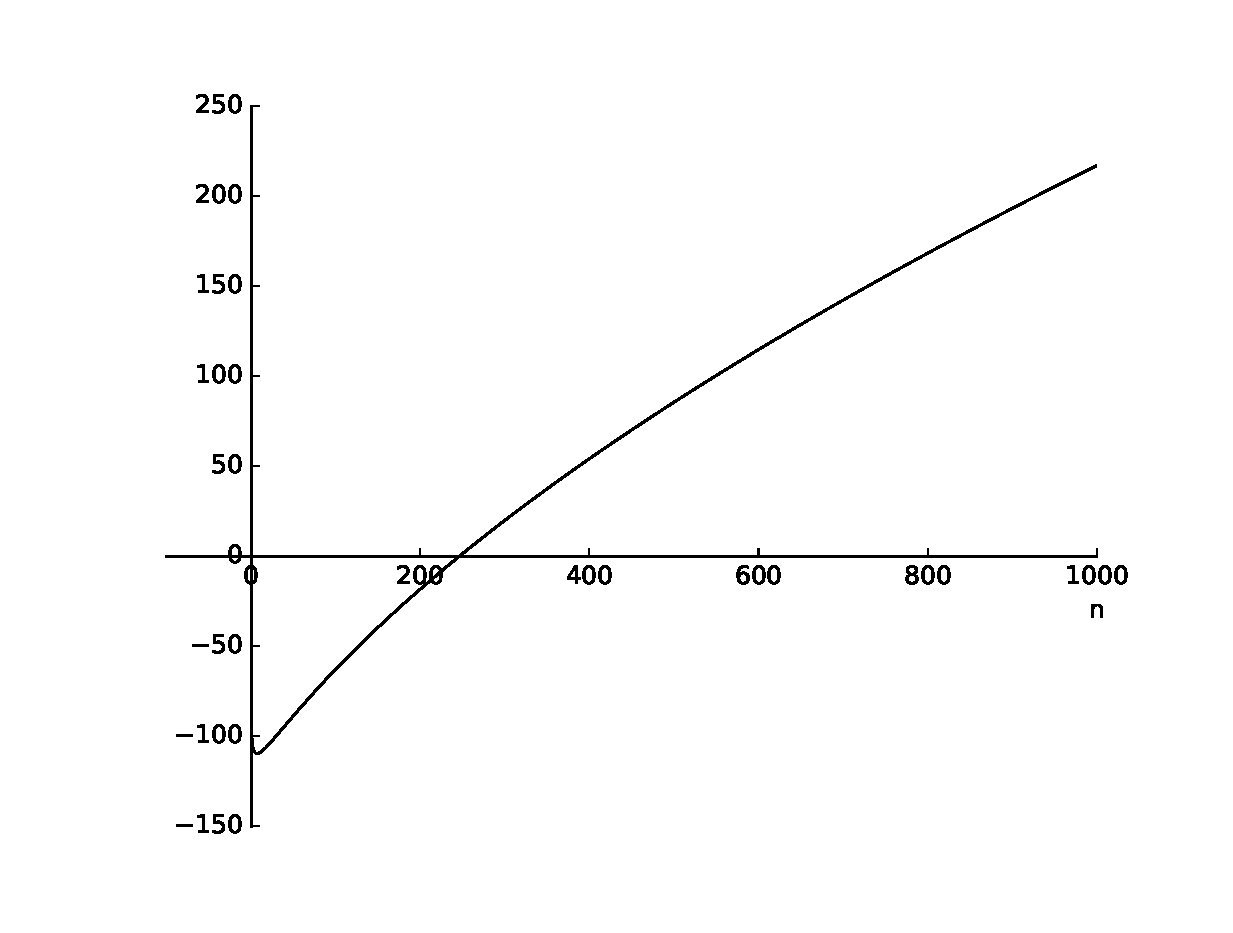
\includegraphics[scale=.25]{intro/sign_size}
%	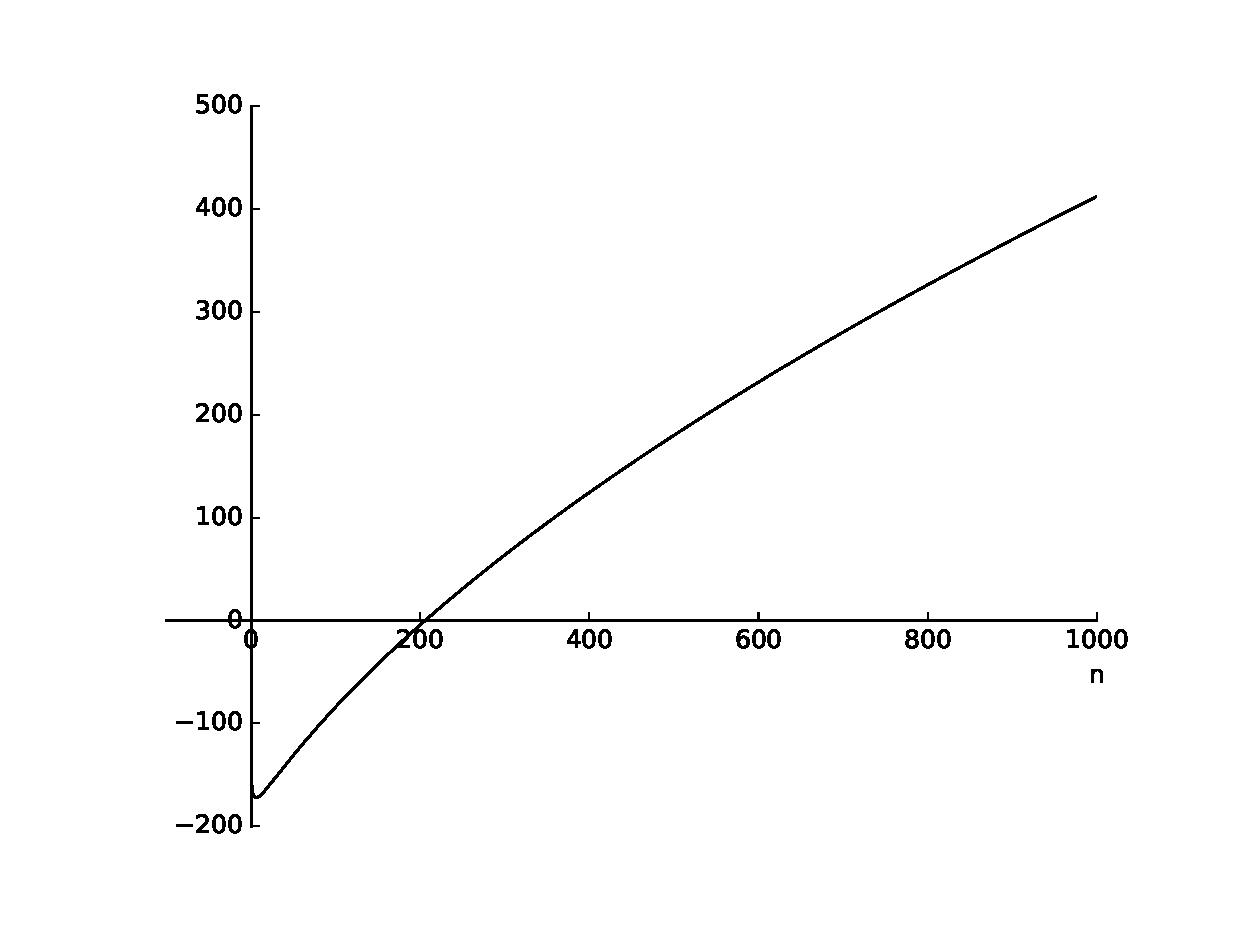
\includegraphics[scale=.25]{intro/sign_time}
%	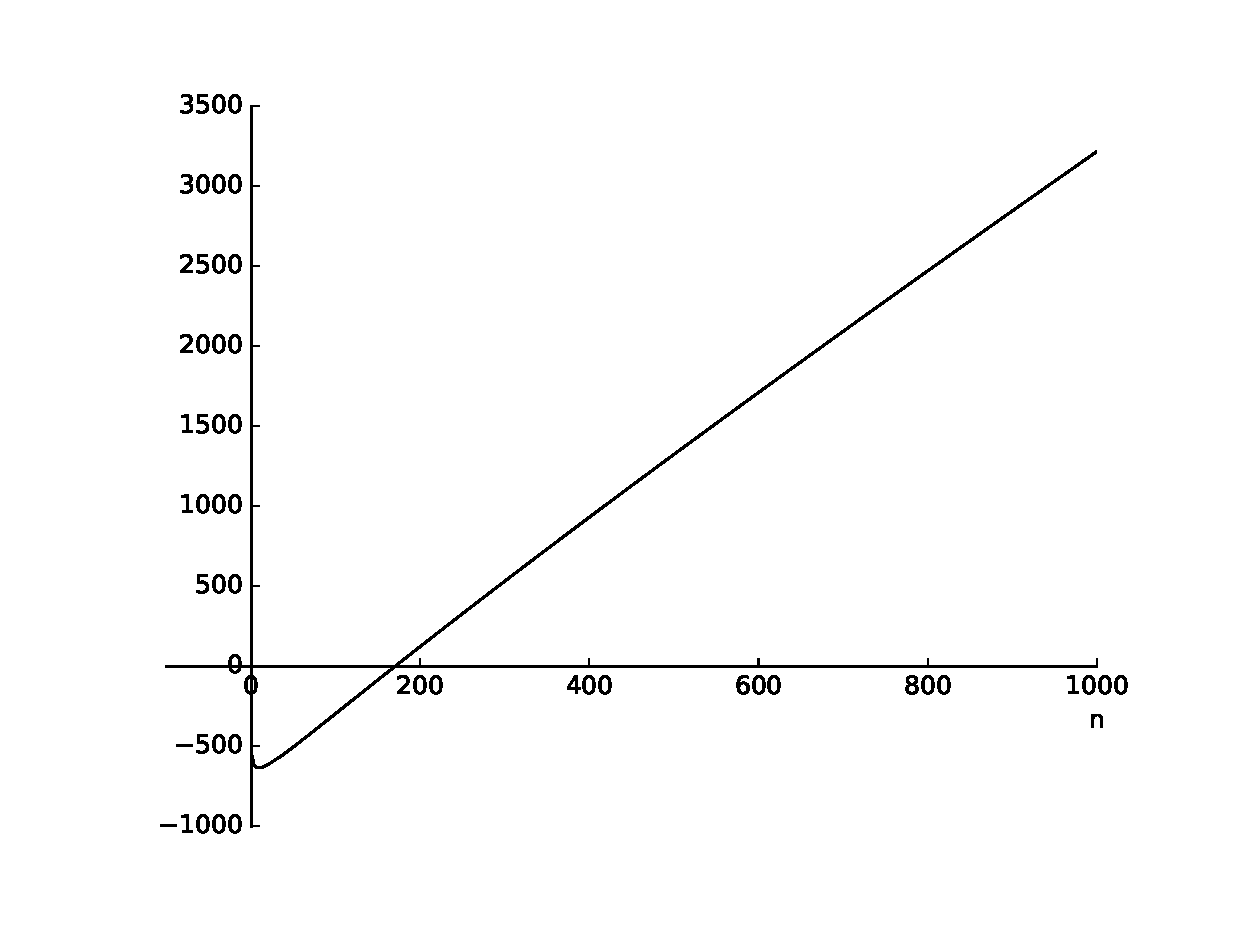
\includegraphics[scale=.25]{intro/ver_time}
%\end{figure} 

   \subsection{Technical Overview} \label{sec:tech-overview}

	% !TEX root = ../main-ring-signature.tex

To give a more clear understanding our contributions, it will be illustrative to see what is the main difficulty when constructing a ring signature on bilinear groups. Most schemes have followed the following approach. Given a ring of users defined by the set of their public keys and a message: a) sign the message, b) prove in zero-knowledge knowledge of a signature which can be verified using some committed/randomized verification key, and then c) prove in zero-knowledge that this verification key belongs to the set of public keys in the ring.  The most expensive part is c) and is sometimes called a \emph{set-membership proof}.

In the case of a ring signature, a set-membership has the following additional property: \emph{all the verification keys forming the ring are honestly generated}. 
Indeed, since the set-membership proof is only used to guarantee unforgeability, it makes no sense to guarantee unforgeability when members of the ring are controlled by the adversary.
It turns out that all the schemes we are aware of, in particular Chandran et al.'s, obviate this property, meaning that their set membership proofs are for adversarially chosen verification keys.
We ask the following natural question.
\begin{displayquote}
Can we construct more efficient set membership proofs (without random oracles or non-falsifiable assumptions) when verification keys are sampled from a known distribution?
\end{displayquote}
We answer this question in the affirmative and we construct a $\Theta(\sqrt[3]{n})$ set membership proof when the verification keys are honestly sampled. In contrast, Chandran et al.'s proof is of size $\Theta(\sqrt{n})$ but it makes no assumption on the verification keys distribution.

Our main technical tool is a structure preserving --- i.e.~compatible with Groth-Sahai proofs --- hash function with \emph{always second-preimage resistance} (aSec in the terminology of Rogaway and Shrimpton \cite{FSE:RogShr04}). That is, given $A$ in the domain of $h$, is hard to find $A'\neq A$ such that $h(A')=h(A)$ {\bf whenever $A$ is randomly sampled from the domain}.
Our function $h$ takes as input $A$, a set of verification keys (in fact, a fragment of each verification key), and returns a constant size digest which is simply $h(A)= \sum_{\vecb{a} \in A} \vecb{a}$. Thereby, whenever $h$ is applied to a set of honestly sampled verification keys, $A$ is indeed random and hence is infeasible to compute a second preimage.

\subsubsection{High level description}
We construct a set membership proof where a prover wants to convince a verifier that some commitment $c$ opens to $\vecb{a}$ and $\vecb{a}\in\{\vecb{a}_1,\ldots,\vecb{a}_n\}$. To do so, we arrange the $n$ elements of the ring into $n^{2/3}$ blocks of size $m=\sqrt[3]{n}$. We coin the following notation: for a ring $\{\vecb{a}_i:1\leq i \leq n\}$ define $\vecb{a}_{\mu,\nu}:=\vecb{a}_{(\mu-1)m+\nu}$, where  $1\leq\mu\leq n^{2/3},1\leq \nu\leq m$.  Let
\begin{align*}
& A_1 := \{\vecb{a}_{1,1},\ldots,\vecb{a}_{1,m}\},\ldots, A_{n^{2/3}} := \{\vecb{a}_{n^{2/3},1},\ldots,\vecb{a}_{n^{2/3},m}\},\,
H:=\{h(A_1),\ldots,\allowbreak h(A_{n^{2/3}})\}.
\end{align*}

We use Chandran et al.'s underlying set membership proof of size $\Theta(\sqrt{n})$ to prove knowledge of some $h(A_\mu)\in H$. Since $|H|=n^{2/3}$, this proof is of size $\Theta(\sqrt[3]{n})$. Then we prove knowledge of $A'$, a preimage of $h(A_\mu)$, which using Groth-Sahai proofs requires commitments to the $\sqrt[3]{n}$ verification keys in the preimage of $h(A_\mu)$ plus a $\Theta(1)$ proof that $h(A')=h(A_\mu)$. Hence, the total size of the proof adds up to $\Theta(\sqrt[3]{n})$ group elements.

Another nice property of our hash function is that its inputs are sets (or equivalently, is invariant under permutations of the input). Hence, we can sort the commitments of the $\sqrt[3]{n}$ verification keys in $A_\mu$ so that the first commitment is $c$. We conclude that $A'=A_\mu$, unless we break second-preimage resistance of $h$, and thus $a$, the opening of $c$, belongs to $\{\vecb{a}_1,\ldots,\vecb{a}_n\}$.

In our ring signature, the verification key will contain $\vecb{a}$ and $vk$, where $vk$ the verification key of a (normal) signature scheme. With the help of another collision-resistant and structure preserving hash function that relates $\vecb{a}$ and $vk$ we will also prove that $vk\in\{vk_1,\ldots,vk_n\}$. We postpone further details to Section \ref{sec:high-level}.

    %\subsection{Discussion}

    	\subsubsection{Extending our technique.}
A natural question is if this technique can be applied once again. That is, to compute a $\Theta(\sqrt[4]{n})$  proof, compute commitments to an element from $H=\{h(A_1),\ldots,h(A_{n^{3/4}})\}$ and
$G=\allowbreak\{
	g_{[\matr{A_1}]}
		([
			\vecb{\kappa}_1]),
	\ldots,\allowbreak
	g_{[\matr{A}_{n^3/4}]}
		([
			\vecb{\kappa}_{n^{3/4}}
])\}$,
and then prove that they belong to the respective sets with our set-membership proof of size $\Theta(\sqrt[3]{n})$. Since $|H|=|G|=n^{3/4}$, the proof will be of size $\Theta(\sqrt[3]{n^{3/4}})=\Theta(\sqrt[4]{n})$. However, this is not possible since the $\Theta(\sqrt[3]{n})$ proof is not a set-membership proof for arbitrary sets but only for sets where each element is of the form $([vk],\vecb{a}[vk],[\vecb{a}])$. Clearly, elements from $H$ and $G'$ do not have this form.


\subsubsection{Erasures.}
In the security proof we need to embed a random preimage $A=\{[\vecb{a}_1],\ldots,\allowbreak [\vecb{a}_{q_{\mathsf{gen}}}]\}$ of $h$ in the verification keys while, where $q_{\mathsf{gen}}$ is the total number of verification keys. On the other hand, the adversary may adaptively corrupt parties obtaining all the random coins used to generate the verification key. That is, we need to reveal $\vecb{a}_i$ (the discrete logs of $[\vecb{a}_i]$) to the adversary, which is incompatible with the permutation pairing assumption and thus with the security of $h$. Since is not clear how to obliviously sample $[\vecb{a}_i]=([a_{i,1}],[a_{i,1}^2])^\top$ and we can only guess the set of corrupted parties with negligible probability, we are forced to use erasures. That is, after sampling $\vecb{a}\gets\mathcal{Q}$ and computing $[\vecb{a}]$, the key generation algorithm erases $\vecb{a}$.

\subsubsection{Getting rid of the non-standard assumptions.} Gonzalez et al.~\cite{ACNS:GonRaf16} modify Groth and Lu's proof of correctness of a shuffle \cite{AC:GroLu07} to get rid of the permutation pairing assumption. They showed that the statement ``$[\vecb{z}_1],\ldots,[\vecb{z}_m]$ is a permutation of $[\vecb{a}_1],\ldots,[\vecb{a}_m]$'', i.e.~$\{[\vecb{a}_1],\ldots,[\vecb{a}_m]\}=\{[\vecb{z}_1],\ldots,[\vecb{z}_m]\}$, can be showed with a proof that $[\vecb{z}_1],\ldots,[\vecb{z}_m]\in\{[\vecb{a}_1],\ldots,[\vecb{a}_m]\}$ and a proof that $\sum_{i=1}^m [\vecb{z}_i]=\sum_{i=1}^m [\vecb{a}_i]$.  Gonzalez et al.~construct a $\Theta(m)$ proof that $[\vecb{z}_1],\ldots,[\vecb{z}_m]\in\{[\vecb{a}_1],\ldots\allowbreak,[\vecb{a}_m]\}$ under standard assumptions (DLin in symmetric groups)  and also noted that finding an element on the kernel of $\matr{A}$ is harder than DLin if $\vecb{a}_1,\ldots,\vecb{a}_m\gets\Z_q^2$.

If we use Gonzalez et al.'s techniques we would have to show that for all $[\vecb{a}']\in A',$ $[\vecb{a}']\in A_ \mu$. However, we can't do this since $A_\mu$ is unknown to the verifier. Instead, we are using features of the permutation pairing assumption that where ignored by Gonzalez et al.~and by Groth and Lu. Indeed, the permutation pairing assumption allows to prove that given $h(A_\mu)$ is infeasible to compute a preimage different than $A_\mu$. We use this fact to commit to $A_\mu$ using a constant number of group elements, while still being able to prove that $A'=A_\mu$%\footnote{We can also see this fact as a group to group length-reducing and computationally binding commitment, which are known to not exists \cite{}} 

\subsubsection{Relation to \cite{AC:GonHevRaf15}.}
Our construction is similar to the set membership proof of Gonzalez et al.~{\cite[Appendix D.2]{AC:GonHevRaf15}. However, the proof system from \cite{AC:GonHevRaf15} does not suffice for constructing a ring signature because there the CRS is fixed to a specific set and thus, the resulting ring signature will be fixed to a specific ring. 






\section{Preliminaries}

	We write PPT as a shortcut for probabilistic polynomial time Turing machine.

Let $\ggen_s$ be some probabilistic polynomial time algorithm which on input $1^{\lambda}$, where $\lambda$ is the security parameter, returns the \emph{group key} which is the description of a symmetric bilinear group $gk:=(q,\GG,\GG_T,e,\mathcal{P})$, where $\GG$
and $\GG_T$ are groups of prime order $q$, the element $\mathcal{P}$ is a generator of 
$\GG$, and $e:\GG\times\GG\to\GG_T$ is an efficiently computable and non-degenerated bilinear map.

Elements in $\GG$ are denoted implicitly as $[a]:=a \Pt$, where $a\in\Z_q$, and elements in $\GG_T$ are denoted as $[a]_T:=a\cdot e(\Pt,\Pt)$. 
The pairing operation is written as a product $\cdot$, that is $[a] \cdot [b]=[a] [b]=e([a],[b])=[ab]_T$. Vectors and matrices are denoted in boldface. Given a matrix $\matr{T}=(t_{i,j})$, $[\matr{T}]$ is
the natural embedding of $\matr{T}$ in $\GG$, that is, the matrix whose $(i,j)$th entry is $t_{i,j}\mathcal{P}$. Given a matrix $\matr{S}$ with the same number of rows as $\matr{T}$, we define $\matr{S}\cat\matr{T}$ as the concatenation of $\matr{S}$ and $\matr{T}$.

	\subsection{Hardness Assumptions} \label{sec:hardness-ass}

	We will use the permutation pairing assumption, introduced by Groth and Lu.
\begin{definition}[Permutation Pairing Assumption \cite{AC:GroLu07}]\label{def:ppa}
Let $\mathcal{Q}_{m}=\underbrace{\mathcal{Q}\cat\ldots\cat\mathcal{Q}}_{m\text{ times}}$, where concatenation of  distributions is defined in the natural way and 
$$\mathcal{Q}: \vecb{a}=\pmatri{x\\x^2},\quad x\gets\Z_q.$$
We say that the $m$-permutation pairing assumption holds relative to $\G_s$ if for any adversary $\advA$
$$
\Pr\left[
\begin{array}{l}
gk\gets\G_s(1^\lambda);\matr{A}\gets\mathcal{Q}_{m};[\matr{Z}]\gets\advA(gk,[\matr{A}]):\\
\mathrm{(i)} \sum_{i=1}^{m}[\vecb{z}_i]=\sum_{i=1}^{m}[\vecb{a}_i], \mathrm{(ii)}\ \forall 1\leq i\leq m\ [z_{2,i}][1]=[z_{1,i}][z_{1,i}],\\
\text{ and }\matr{Z}\text{ is not a permutation of the columns of }\matr{A}
\end{array}
\right],
$$
where $[\matr{Z}]=[\vecb{z}_1\cat\cdots\cat\vecb{z}_m], [\matr{A}]=[\vecb{a}_1\cat\cdots\cat\vecb{a}_m]\in\GG^{2\times m}$,
is negligible in $\lambda$.
\end{definition}
Groth and Lu proved the hardness of the permutation pairing assumption is generic bilinear groups. 

We recall the definition of the decisional linear assumption (in matrix notation) and the kernel matrix Diffie-Hellman assumption.

\begin{definition}[Decisional Diffie-Hellman Assumption (DLin)]\label{def:dlin}
 Let  $\gk 
\gets \ggen_s(1^\lambda)$ and let
$$
\matr{A} :=
\begin{pmatrix} 
a_1 & 0     \\
0     & a_2 \\
1     &  1
\end{pmatrix},
\quad
a_1,a_2\gets\mathbb{Z}_q.
$$
We say that the DLin assumption holds relative to $\ggen_s$ if for all PPT adversaries $\advD$
$$
\adv_{\mathrm{DLin},\ggen_s}(\advD) := |
	\Pr[
		\advD(
			gk,
			[\matr{A}],
			[\matr{A}\vecb{w}])=1]
	-\Pr[
		\advD(
		gk,
		[\matr{A}],
		[\vecb{z}])=1]|
$$
is negligible in $\lambda$, where the probability is taken over $gk\gets\ggen_s(1^\lambda)$, $a_1,a_2\gets\ZZ_q$, $\vecb{w}\gets\ZZ_q^2$, $[\vecb{z}]\gets\GG^3$, and the coin tosses of the adversary. 
\end{definition}

\begin{definition}[Kernel Diffie-Hellman Assumption in $\GG$ \cite{EPRINT:MorRafVil15}] Let  $\gk 
\gets\ggen_s(1^\lambda)$ and $\dist_{\ell,k}$ a distribution over $\Z_q^{\ell\times k}$.
The Kernel Diffie-Hellman assumption in $\GG$ ($\dist_{\ell,k}\mbox{-}\kermdh_{\GG}$) says that every PPT Algorithm has negligible advantage in the following  game: given $[\matr{A}]$, where $\matrA \gets \dist_{\ell,k}$, find $[\vecb{x}] \in \GG^{\ell}$, $\vecb{x} \neq \vecb{0}$, such that 
$[\vecb{x}]^{\top}[\matr{A}]=[\vecb{0}]_T$. 
\end{definition}

We will be using the $Q_m^\top\mbox{-}\kermdh$ assumption, which was proven secure in the generic bilinear group model by Groth and Lu \cite{AC:GroLu07}.

		\subsection{Ring Signature Definition}
    
            		We follow Chandran et al.'s definitions \cite{ICALP:ChaGroSah07}, which extends the original definition of Bender et al. \cite{TCC:BenKatMor06} by including a CRS and perfect anonymity. We allow erasures in the key generation algorithm.

\begin{definition}[Ring Signature]
A ring signature scheme consists of a quadruple of
PPT algorithms $(\mathsf{CRSGen}, \KG, \mathsf{Sign}, \mathsf{Verify})$ that respectively, generate the common
reference string, generate keys for a user, sign a message, and verify the signature of a
message. More formally:
\begin{itemize}
\item $\mathsf{CRSGen}(gk)$, where $gk$ is the group key, outputs the common reference
string $\rho$.
\item $\KG(\rho)$ is run by the user. It outputs a public verification key $vk$ and a private
signing key $sk$.
\item $\mathsf{Sign}_{\rho,sk}(m, R)$ outputs a signature $\sigma$ on the message $m$ with respect to the ring
$R = \{vk_1,\ldots,vk_n\}$. We require that $(vk, sk)$ is a valid key-pair output by $\KG$
and that $vk \in R$.
\item $\mathsf{Verify}_{\rho,R}(m, \sigma)$ verifies a purported signature $\sigma$ on a message $m$ with respect to
the ring of public keys $R$ and reference string $\rho$. It outputs 1 if $\sigma$ is a valid signature for $m$ with respect to $R$  and $\rho$, and 0 otherwise.
\end{itemize}
The quadruple $(\mathsf{CRSGen}, \KG, \mathsf{Sign}, \mathsf{Verify})$ is a ring signature with perfect
anonymity if it has perfect correctness, computational unforgeability and perfect
anonymity as defined below.
\end{definition}

\begin{definition}[Perfect Correctness]
We require that a user can sign any message on behalf of a ring where she is a member. A ring signature $(\mathsf{CRSGen},\allowbreak \KG, \mathsf{Sign}, \mathsf{Verify})$
has perfect correctness if for any unbounded adversary $\advA$ we have:
$$
\Pr\left[\begin{array}{l}
gk\gets\G(1^\lambda);\rho\gets\mathsf{CRSGen}(gk);(vk,sk)\gets\KG(\rho);\\
(m,R)\gets\advA(\rho,vk,sk);\sigma\gets\mathsf{Sign}_{\rho,sk}(m;R):\\
\mathsf{Verify}_{\rho,R}(m,\sigma)=1\text{ or }vk\notin R
\end{array}\right]=1
$$
\end{definition}

\begin{definition}[Computational Unforgeability]
A ring signature scheme $(\mathsf{CRSGen}, \KG, \mathsf{Sign}, \mathsf{Verify})$
is unforgeable if it is infeasible to forge a ring
signature on a message without controlling one of the members in the ring. Formally, it
is unforgeable when for any non-uniform polynomial
time adversaries $\advA$ we have that
$$
\Pr\left[\begin{array}{l}
gk\gets\G(1^\lambda);\rho\gets\mathsf{CRSGen}(gk);(m,R,\sigma)\gets\advA^{\mathsf{VKGen},\mathsf{Sign},\mathsf{Corrupt}}(\rho):\\
\mathsf{Verify}_{\rho,R}(m,\sigma)=1
\end{array}\right]
$$
is negligible in th security parameter, where

\begin{itemize}
\item $\mathsf{VKGen}$ on query number $i$ selects randomness $w_i$, computes $(vk_i,sk_i):= \KG(\rho; w_i)$
and returns $vk_i$.
\item $\mathsf{Sign}(i, m, R)$ returns $\sigma \gets \mathsf{Sign}_{\rho,sk_i}(m, R)$, provided $(vk_i, sk_i)$ has been generated
by $\mathsf{VKGen}$ and $vk_i\in R$.
\item $\mathsf{Corrupt}(i)$ returns $sk_i$  provided $(vk_i, sk_i)$ has
been generated by $\mathsf{VKGen}$. (The fact that $w_i$ is not revealed allows the erasure of the random coins used in the generation of $(vk_i, sk_i)$).
\item $\advA$ outputs $(m, R, \sigma)$ such that $\mathsf{Sign}$ has not been queried with $(*, m, R)$ and $R$
only contains keys $vk_i$ generated by $\mathsf{VKGen}$ where $i$ has not been corrupted.
\end{itemize}
\end{definition}

\begin{definition}[Perfect Anonymity]
A ring signature scheme
$(\mathsf{CRSGen},\allowbreak \KG,\allowbreak \mathsf{Sign}, \mathsf{Verify})$ has perfect anonymity, if a signature on a message
$m$ under a ring $R$ and key $vk_{i_0}$
looks exactly the same as a signature on the
message $m$ under the ring $R$ and key $vk_{i_1}$, where $vk_{i_0},vk_{i_1}\in R$. This means that the signer's key is hidden
among all the honestly generated keys in the ring. Formally, we require that for any unbounded
adversary $\advA$:
\begin{align*}
&\Pr\left[\begin{array}{l}
gk\gets\G(1^\lambda);\rho\gets\mathsf{CRSGen}(gk);\\
(m,i_0,i_1,R)\gets\advA^{\KG(\rho)}(\rho);\sigma\gets\mathsf{Sign}_{\rho,sk_{i_0}}(m,R):\\
\advA(\sigma)=1
\end{array}\right]
=\\
&\Pr\left[\begin{array}{l}
gk\gets\G(1^\lambda);\rho\gets\mathsf{CRSGen}(gk);\\
(m,i_0,i_1,R)\gets\advA^{\KG(\rho)}(\rho);\sigma\gets\mathsf{Sign}_{\rho,sk_{i_1}}(m,R):\\
\advA(\sigma)=1
\end{array}\right]
\end{align*}
where $\advA$ chooses $i_0, i_1$ such that $(vk_{i_0}, sk_{i_0}),(vk_{i_1}, sk_{i_1})$ have been generated by the
oracle $\KG(\rho)$.
\end{definition}



	\subsection{Groth-Sahai Proofs in the SXDH Instantiation} \label{sec:gs-proofs}

		% !TEX root = ../main-ring-signature.tex

The Groth Sahai (GS) proof system is a non-interactive witness indistinguishable proof system (and in some cases also zero-knowledge) for the language of quadratic equations over a bilinear group. The admissible equation types must be in the following form:
\begin{equation}\label{gseq}
\sum_{j=1}^{m_y} f(\alpha_j, \vary_j)+\sum_{i=1}^{m_x} f(\varx_i, \beta_i)+\sum_{i=1}^{m_x} \sum_{j=1}^{m_y}  f(\varx_i,\escQE_{i,j} \vary_j)=t,
\end{equation}
 where $\boldsymbol \alpha  \in \Am_1^{m_y}$, $\boldsymbol \beta  \in \Am_2^{m_x}$, $\matr{\EscQE}=(\escQE_{i,j}) \in \Z_q^{m_x\times m_y}$, $t \in \Am_T$, and $\Am_1,\Am_2,\Am_T\in\{\Z_q,\GG_1,\GG_2, \GG_T\}$ 
are equipped with some bilinear map $f:\Am_1\times \Am_2 \rightarrow \Am_T$.

The GS proof system is a \emph{commit-and-prove} proof system, that is, the prover first commits to solutions
of equation (\ref{gseq}) using the GS commitments, and then computes a proof that the committed values satisfies equation (\ref{gseq}).

GS proofs are perfectly sound when the CRS is sampled from the perfectly binding distribution, and perfectly witness-indistinguishable when sampled from the perfectly hiding distribution. Computational indistinguishability of  both distributions implies either perfect soundness and computational witness indistinguishability or computational soundness and perfect witness-indistinguishability.

\subsubsection{Groth-Sahai Commitments.}
Following Groth and Sahai's work \cite{EC:GroSah08}, in symmetric groups and using the SXDH assumption, GS commitments are vectors in $\GG^2_1$ or $\GG_2^2$ of the form
\begin{align*}
&\GS.\Com_{ck_1}([x]_1;\vecb{r}):=\pmatri{{[0]_1}\\{[x]_1}}+r_1[\vecb{u}_1]_1+{r}_2[\vecb{u}_2]_1\\
&\GS.\Com_{ck_1}(x;\vecb{r}):=x\left([\vecb{u}_1]_1+\pmatri{{[0]_1}\\{[1]_1}}\right)+{r}[\vecb{u}_2]_1\\
& \GS.\Com_{ck_2}([x]_2;\vecb{r}):=\pmatri{{[0]_2}\\{[x]_2}}+r_1[\vecb{v}_1]_2+{r}_2[\vecb{v}_2]_2\\
&\GS.\Com_{ck_2}(x;\vecb{r}):=x\left([\vecb{v}_1]_2+\pmatri{{[0]_2}\\{[1]_2}}\right)+{r}[\vecb{v}_2]_2
\end{align*}
where $ck_1:=[\vecb{u}_1\cat\vecb{u}_2]_1,ck_2:=[\vecb{v}_1\cat\vecb{v}_2]_2$, and $\vecb{u}_2,\vecb{v}_2$ are sampled from the same distribution as $\matr{A}$, the matrix from definition \ref{def:dlin}. The GS reference string is formed by the commitment keys $ck_1,ck_2$  and $\vecb{u}_1:=w\vecb{u}_2\vecb{v}_1:=w'\vecb{v}_2$ in the perfectly binding setting, and $\vecb{u}_1:=w\vecb{u}_2-\vecb{e}_2,\vecb{v}_1:=w'\vecb{v}_2-\vecb{v}_2$ in the perfectly hiding setting, for $w,w'\gets\Z_q$.


	\subsection{Boneh-Boyen Signatures} \label{sec:bbs}
    
            % !TEX root = ../main-ring-signature.tex


Boneh and Boyen introduced a short signature --- each signature consists of only one group element --- which is secure against existential forgery under weak chosen message attacks without random oracles \cite{EC:BonBoy04a}.
The verification of the validity of any signature-message pair can be written as a set of pairing product equations. Thereby, using Groth-Sahai proofs one can show the possession of a valid signature without revealing the actual signature.

We construct our ring signature using Boneh-Boyen signatures, but we could replace the Boneh-Boyen signature scheme with a structure preserving signature scheme secure under milder assumptions (e.g.~\cite{EPRINT:JutRoy17}). We rather keep it simple and stick to Boneh-Boyen signature which, since the verification key is just one group element, simplifies the notation and reduces the size of the final signature.
 
\begin{definition}[weak Existential Unforgeability (wUF-CMA)] We say that a signature scheme $\Sigma = (\mathsf{KGen},\mathsf{Sign},\mathsf{Ver})$ is wUF-CMA if for any PPT adversary $\advA$
	$$
	\Pr\left[\begin{array}{l}
	gk \gets \ggen_a(1^\lambda), (m_1,\ldots,m_{q_\mathsf{sig}})\gets\advA(gk), (sk,vk)\gets\KGen(1^\lambda), \\
	(m,\sigma)\gets\advA(\Sign_{sk}(m_1),\ldots,\Sign_{sk}(m_{q_\mathsf{sig}})):\\
	\Ver_{vk}(m,\sigma)=1 \text{ and } m\notin \{m_1,\ldots,m_{q_\mathsf{sig}}\}
	\end{array}\right]
	$$
is negligible in $\lambda$.
\end{definition}

The Boneh-Boyen signature described bellow is wUF-CMA under the $m$-\emph{strong Diffie-Hellman} assumption.
%which is described below.
%
%\begin{definition}[$m\mbox{-}SDH$ assumption]
%For any PPT adversary $\advA$
%$$
%\Pr\left[gk\gets\G_a(1^\lambda),x\gets\Z_q:\advA(gk,[x]_{3-s},[x]_s,[x^2]_s,\ldots,[x^m]_s)=(c,\left[\frac{1}{x+c}\right]_s)\right]
%$$
%s negligible in $\lambda$.
%\end{definition}
%
%Given $s\in\{1,2\}$, the Boneh-Boyen signature scheme is described below.

\begin{description}
\item[$\mathsf{BB}.\KG$:] Given a group key $gk$, pick $vk\gets\Z_q$. The secret/public key pair is defined as $(sk,vk):=(x,[x]_{3-s})$.
\item[$\mathsf{BB}.\Sign$:] Given a secret key $sk\in\Z_q$ and a message $m\in\Z_q$, output the signature $[\sigma]_{s}:=\left[\frac{1}{x+m}\right]_{s}$. In the unlikely case that $x+m=0$ we let $[\sigma]_{s}:=[0]_{s}$.
\item[$\mathsf{BB}.\Ver$:] On input the verification key $[vk]_{3-s}$, a message $m\in\Z_q$, and a signature $[\sigma]_{s}$, verify that $[m+x]_{3-s}[\sigma]_{s}=[1]_T$.
\end{description} 

It is direct to prove knowledge of a Boneh-Boyen signature for some message $m$ under some committed verification key with a Groth-Sahai proof for the verification equation. In our SXDH based ring signature we need to prove a slightly different statement. Since we have a commitment to the secret key $[\vecb{c}]_{2} = \Com_{ck_2}(x;s) = x[\vecb{w}_1]_2+s[\vecb{w}_2]_2$ we need to show that
\begin{equation}
e([{\sigma}]_1, m[\vecb{w}_1]_2 + [\vecb{c}]_2) - [\vecb{w}_1]_T= e([s]_1,[w_2]_2),
\label{eq:bbs-verification}
\end{equation}
for some $s\in\Z_q$.


      	\subsection{Chandran et al.'s Set-Membership Proof} \label{sec:chan-rs}
	
       		%!TeX root=../main_ring_signature.tex
Consider a {Boneh-Boyen signature scheme} with secret/verification keys of the form $(sk,[vk])$ and a {one-time signature scheme}. The signature of the message $m$ for a ring $R=\{[vk_1],\ldots,[vk_n]\}$ is computed as follows:
\begin{itemize}
	\item[a)] Pick a one-time signature key $(sk_\mathsf{ot},vk_\mathsf{ot})$, sign $m$ with $sk_\mathsf{ot}$, and sign $vk_\mathsf{ot}$ with $sk$.
	\item[b)] Show possession of valid signature of $vk_\mathsf{ot}$ under $[vk]$ using Groth-Sahai proofs.
	\item[c)] Show that $[vk]\in R$.
\end{itemize}
The most expensive part is c) and the core of Chandran et al.'s construction is a proof of size $\Theta(\sqrt{n})$ of c). We call this kind of proof a set-membership proof and we describe Chandran et al.'s below.
 
The proof arranges the set of verification keys on a matrix of size $m\times m$, where $m:=\sqrt{n}$, as depicted below
$$
[\matr{V}]:=
\begin{pmatrix}
[vk_{1,1}] & \cdots & [vk_{1,m}]\\
\vdots     & \ddots & \vdots \\
[vk_{m,1}]  & \cdots & [vk_{m,m}],
\end{pmatrix}
$$
where $vk_{i,j}:=vk_{(i-1)m+j}$ for $1\leq i,j \leq m$.

Let $[vk_\alpha]$ the verification key for which the prover wants to show that $[vk_\alpha]\in R$ and let $i_\alpha,j_\alpha$ such that $vk_\alpha = vk_{i_\alpha,j_\alpha}$. The prover selects the $j_\alpha$ th column of $[\matr{V}]$ and then the $i_\alpha$ th element of that column. To do so, the prover commits to 
\begin{enumerate}
\item $b_1,\ldots,b_m\in\bits$ such that $b_j=1$ iff $j=j_\alpha$,
\item $b'_1,\ldots,b'_m\in\bits$ such that $b'_i=1$ iff $i=i_\alpha$,
\item $[\kappa_1]:=[vk_{1,j_\alpha}],\ldots,[\kappa_m]:=[vk_{m,j_\alpha}]$.
\end{enumerate}

Using Groth-Sahai proofs, the prover proves that
\begin{enumerate}[i.]
\item $b_1(b_1-1)=0,\ldots,b_m(b_m-1)=0,b'_1(b'_m-1)=0,\ldots,b'_m(b'_m-1)=0$,\label{eq1}
\item $\sum_{i=1}^m b_i =1$ and $\sum_{i=1}^m b'_i=1$,\label{eq2}
\item $[\kappa_1]=\sum_{j=1}^m b_j [vk_{1,j}],\ldots,[\kappa_m]=\sum_{j=1}^m b_j[vk_{m,j}]$,\label{eq3}
\item $[vk_\alpha]=\sum_{i=1}^m b'_i[\kappa_i]$.\label{eq4}
\end{enumerate}
Equations \ref{eq1} and \ref{eq2} prove that $(b_1,\ldots,b_m)$ and $(b'_1,\ldots,b'_m)$ are unitary vectors, equation \ref{eq3} proves that $([\kappa_1],\ldots,[\kappa_m])^\top$ is a column of $[\matr{V}]$, and equation \ref{eq4} proves that $[vk_\alpha]$ is an element of $([\kappa_1],\ldots,[\kappa_m])$.

	\subsection{Hash Functions} \label{sec:hash}

		% !TEX root = ../main-ring-signature.tex

We recall the definition of a hash function plus three variants: a stronger variant where  the adversary may adaptively ask for the random coins of parts of the key, and a weaker notion where the adversary needs to find a second preimage, and another notion where the adversary can choose its own key meeting some restrictions.\footnote{See the work of Rogaway and Shrimpton \cite{FSE:RogShr04} for several notions collision resistance and their relations. Adaptivity and Key-Flexibility is not considered though.} We consider functions $h,g:\mathcal{K}\times\mathcal{M}\to\mathcal{Y}$ and an algorithm $\KGen$ which on input a group key randomly samples an element from $\mathcal{K}$.

We say that $h$'s key can be generated in a distributed fashion if $h:\mathcal{K}_\mathsf{global}\times\mathcal{K}^m_{\mathsf{local}}\times\mathcal{M}^m\to \mathcal{Y}$, $\KGen = (\KGen_\mathsf{global},\KGen_\mathsf{local})$, the key is of the form $k = (k_0,k_1,\ldots,k_m)$ and the input is of the form $x=(x_1,\ldots,x_m)$, where $k_0\gets\KGen_{\mathsf{global}}(gk)$, $k_i\gets\KGen_{\mathsf{local}}(gk,k_0,\mathsf{aux}_i)$, $\mathsf{aux}_1,\ldots,\mathsf{aux}_m$ are auxiliary inputs, and $i\in[m]$. 

In our instantiations with the SXDH assumption we will need to relax the collision condition. We do so by relaxing the equality relation to different ad-hoc equivalence relations. For example, we consider that $x,x'$ are a collision if, besides $x\neq x'$, $x$ and $x'$ are commitments which can't be opened to the same value.

\begin{definition}[Collision Resistance]\label{def:hash1}
 We say that $h$ is a hash-function family with collision resistance if for all PPT adversary $\advA$
$$
\adv_g^{\mathsf{Col}}(\advA) := \Pr[k\gets\KGen(1^\lambda), (x,x')\gets \advA(k):x\neq x'\text{ and }h_k(x)=h_k(x')]
$$ 
is negligible in $\lambda$.
\label{def:collision-resistance}
\end{definition}

For functions whose key is generated in a distributed fashion, we consider a stronger notion of collision resistance which we call adaptive collision resistance. We refer to definition \ref{def:collision-resistance} as static collision resistance.


\begin{definition}[Adaptive Collision Resistance] \label{def:hash1-adaptive}
A hash-function family $h$ with distributed key generation is adaptive collision resistant if for all PPT adversary $\advA$
$$
\adv_g^{\mathsf{aCol}}(\advA) := \Pr\left[\begin{array}{c}
k_0\gets\KGen_{\mathsf{global}}(gk), (x,x')\gets \advA^{\mathsf{KeyGen},\mathsf{Corrupt}}(k_0):\\
x_{I\setminus Q} \neq x_{I\setminus Q}\text{ and }h_k(x)=h_k(x')
\end{array}\right]
$$ 
is negligible in $\lambda$.  The $i$-th call to the oracle $\mathsf{KeyGen}(\mathsf{aux}_i)$ stores $i$ on $I$, if $i\notin I$, and returns $k_i:=\KGen(gk,k_0,\mathsf{aux}_i;r_i)$, for a uniform $r_i\in\bits^{\mathsf{poly}(\lambda)}$. The oracle $\mathsf{Corrupt}(i)$ returns the random coins used to generate $k_i$, if $i\in I$, and stores $i$ in $Q$. For an index set $S  = \{s_1,\ldots,s_n\}$, condition $x_{S} \neq x'_{S}$ means that $(x_{s_1},\ldots, x_{s_n})\neq (x'_{s_1},\ldots,x'_{s_n})$. 
\end{definition}

We use a weaker variant of collision resistance for our hash function based on the PPA assumption.

\begin{definition}[Second-Preimage Resistance]\label{def:hash2}
 We say that $h$ is a hash-function family with always second-preimage resistance if for all PPT adversary $\advA$
$$
\adv_h^{\mathsf{Sec}}(\advA) := \Pr\left[\begin{array}{c}
k\gets\KGen(gk), x\gets\mathcal{M}, x'\gets A(k,x):\\
 x\neq x'\text{ and }h_k(x)=h_k(x')
 \end{array}\right]
$$ 
is negligible in $\lambda$.
\end{definition}
%We also define an adaptive variant of second-preimage resistance  which consider attacks were the adversary computes its own key $k'$ such that $g_{k'}(x') = g_{k}(x)$. We require that $k\sim k'$, where $\sim\subset \mathcal{K}\times\mathcal{K}$ is an equivalence relation (in our ring signature we will consider $k\sim k\iff h(k)=h(k')$, for another collision resistance hash function $h$)
%
%\begin{definition}[Key-Flexible Adaptive Second-Preimage Resistance]\label{def:KaSec}
% A hash-function family $h$ with distributed key generation is adaptive second-preimage resistant if for all PPT adversary $\advA$
%$$
%\adv_g^{\mathsf{KaSec}}(\advA) := \Pr\left[\begin{array}{c}
%k_0\gets\KGen_{\mathsf{global}}(gk), x\gets\mathcal{M},(k',x')\gets \advA^{\mathsf{KeyGen},\mathsf{Corrupt}}(k_0):\\
%k\sim k', x_{I\setminus Q} \neq x_{I\setminus Q}\text{ and }g_k(x)=g_k(x')
%\end{array}\right]
%$$ 
%is negligible in $\lambda$.  The $i$-th call to the oracle $\mathsf{KeyGen}(\mathsf{aux}_i)$ stores $i$ on $I$, if $i\notin I$, and returns $k_i:=\KGen(gk,k_0,\mathsf{aux}_i;r_i)$, for a uniform $r_i\in\bits^{\mathsf{poly}(\lambda)}$. The oracle $\mathsf{Corrupt}(i)$ returns the random coins used to generate $k_i$, if $i\in I$, and stores $i$ in $Q$. For an index set $S  = \{s_1,\ldots,s_n\}$, condition $x_{S} \neq x'_{S}$ means that $(x_{s_1},\ldots, x_{s_n})\neq (x'_{s_1},\ldots,x'_{s_n})$. 
%\end{definition}

    \section{Our Construction in the PPA setting} \label{sec:hf}
    
    	% !TEX root = ../main-ring-signature.tex

In this section we construct two different (but related) hash functions. The functions $g$ and $h$ defined in section \ref{sec:hf-ppa}  are proven collision resistant under the PPA (and the $\kermdh$) assumption. In section \ref{sec:hf-sxdh} we give another pair of functions $g$ and $h$ which we prove collision resistant under the SXDH assumtion.

Collision resistance of functions from section \ref{sec:hf-ppa} are almost direct consequence of the PPA assumption, while the functions from \ref{sec:hf-sxdh} are inspired on the PPA instantiations but are more complex. For example, neither $h$ and $g$ are efficiently computable, but we manage to prove that $h(x)=h(x')$ and $g_k(x)=h_k(x')$ for concrete values encoded in $g$'s key $k$. 

Function $h$ in the SXDH setting is unconditionally collision resistant under a relaxation of the notion of equality of purported collisions. Note that unconditionality implies that collision resistance holds with respect to any auxiliary information (in particular $k$). On the other hand, function $h$ in the PPA instantiation is only second-preimage collision resistant.

For both functions $g$, $k$ is computed in a distributed fashion $k = (k_0,k_1,\ldots,k_n)$, such that $k_i$ is computed only from $k_0$ and hence, if $j\neq i$, then $k_i$ and $k_j$ are independent conditioned on $k_0$. In our ring signature, $k_0$ will be the global reference string and $k_i$ will be the verification key which is locally computed by the $i$-th party. 
Function $g$ is adaptive collision resistant under the SXDH assumption, while the PPA instantiation is only statically collision resistant.

%We additionally show how to compute zero-knowledge proofs of membership in the message space of $h$ and of satisfiability of $g_k(x)=g_k(x')$.
%We obtain shorter proofs replacing some commitments by ElGamal encryptions as done in \cite{PKC:EscGro14}. Although the security of this shorter proofs is shown in \cite{PKC:EscGro14}, for completeness we include in Appendix XXX the security proofs of our instantiations of the general framwork described in \cite{PKC:EscGro14}.
    	
    	\subsection{Our hash functions from the PPA assumption} \label{sec:hf-ppa}
    	
    		% !TEX root = ../main-ring-signature.tex

We instantiate definition \ref{def:hash1} with the function $g$ and \ref{def:hash2}  with $h$ defined as follows. For  $h$, $\mathcal{M}=Q_m$, $\mathcal{Y}=\GG_1^2$, $\KGen=\ggen_a$, and
\begin{align*}
&h(A):= \sum_{([\vecb{a}]_1,[\vecb{a}]_2)\in A}[\vecb{a}]_1, \text{ where}\\
&\mathcal{Q}_m := \{\matr{A}\in \Z_q^{2\times m}:A=(\vecb{a}_1\cat\cdots\cat\vecb{a}_m) \text{ and } \vecb{a}_i = (a_{i,1},a_{i,2})^\top \text{ s.t. } a_{i,2} = a_{i,1}^2\}\text{ and }\\
&Q_m = \{A : \exists \matr{A}\in\mathcal{Q}_m\text{ s.t. } A' = \cup_{i=1}^m([\vecb{a}_i]_1,[\vecb{a}_i]_2)\}.
\end{align*}
It might seem odd to define $Q_m$ as sets  of vectors in both groups while $h$ only require elements in one group. However, this will be crucial in the security proof of our ring signature, where we need to compute $[vk \vecb{a}]_2$, for some $vk\in\Z_q$, without knowledge of $\vecb{a}$. For simplicity, we may just write $h(A)$ for $A\subseteq \GG_1^2$ (which is still well defined).

Given a second preimage $h$, it is trivial to construct an adversary breaking the $m$-PPA assumption. Indeed, Let $[\matr{A}]_1,[\matr{A}]_2$ the challenge of the $m$-PPA assumption and let $A$ the set of columns of $[\matr{A}]_1$ and $[\matr{A}]_2$, which is clearly uniformly distributed in $Q_m$. Then given any $A'\in Q_m$ such that $A'\neq A$ and $h(A)=h(A')$, it holds that $[\matr{A}']_1$, the matrix whose columns are the first components of the elements of $A'$, is not a permutation of $[\matr{A}]_1$ and hence breaks $m$-PPA assumption. Then for any adversary $\advA$ there is an adversary $\advB$ such that $\adv^{\mathsf{aPre}_g}(\advA)=\adv_{m\mbox{-}\mathsf{PPA}}(\advB)$. 

In the case of $g$, $\mathcal{M}=\GG^m_2$, $\mathcal{Y}=\GG_2^2$, and $\KGen_{\mathsf{global}}$ picks a group description $gk\gets\ggen_a(1^\lambda)$, while $\KGen_\mathsf{local}$ picks $[\vecb{a}]_1\in\GG^{2\times m}_1$, where $\vecb{a}\gets\mathcal{Q}_1$, and the function is defined as
$$
g_{[\matr{A}]_1}([\vecb{x}]_2):= [\matr{A}\vecb{x}]_2.
$$
Although not efficiently computable, one can efficiently check if $g_{[\matr{A}]_1}([\vecb{x}]_2) = g_{[\matr{A}]_1}([\vecb{x}']_2)$ using the pairing operation. Further, in our scheme we will publish values of the form $[\vecb{a}_ix_i]_2$ which will render $g$ efficiently computable.

Given a collision $[\vecb{x}]_2,[\vecb{x}']_2$ for $g$, then $([\vecb{x}]_2-[\vecb{x}]'_2)\neq [\vecb{0}]$ is in the kernel of $[\matr{A}]_1$. Therefore, is trivial to prove that for any adversary $\advA$ against static collision resistance there is an adversary $\advB$ such that $\adv^{\mathsf{Col}_g}(\advA)=\adv_{\mathcal{Q}_m^\top\mbox{-}\skermdh}(\advB)$, whenever $\matr{A}\gets\mathcal{Q}_m$.

We note that given $A\in Q_m,[\matr{A}]_1\in\GG^{2\times m}_1,[\vecb{x}]_2\in\GG^m_2$, $[\vecb{y}]_1\in\GG_2^2$ and $[\vecb{y}']_1\in\GG^1_2$ one can express the statements $A\in Q_m$, $g_{[\matr{A}]_1}([\vecb{x}]_2)=[\vecb{y}]_2$, and $h(A)=[\vecb{y}']_1$ as (\ref{eq:Q}),(\ref{eq:g}), and (\ref{eq:h}), respectively.
 \begin{align}
&e([a_{1}]_1,[1]_2) = e([1]_1,[{b}_1]_2)\text{ and }\nonumber\\
&e([a_{2}]_1,[1]_2)=e([a_{1}]_1,[b_1]_2)
\text{ for each }([\vecb{a}]_1,[\vecb{b}]_2)\in A \label{eq:Q}\\
&\sum_{j=1}^m e([a_{i,j}]_1,[x_i]_1) = e([1]_1,[y_i]_2) \text{ for each } i\in\{1,2\} \label{eq:g}\\
&\sum_{([\vecb{a}]_1,[\vecb{a}]_2)\in A} [a_i]_1 = [y'_i]_1 \text{ for each } i\in\{1,2\}.\label{eq:h}
\end{align}
Hence, one can compute Groth-Sahai proofs of size $\Theta(m),\Theta(1)$, and $\Theta(1)$, respectively, for the satisfiability of each statement.

Finally, we prove a simple lemma that relates both functions
\begin{lemma}\label{lemma:hg}
Let $A\gets Q_m,A'\in Q_m,[\vecb{x}]_2,[\vecb{x}']_2\in\GG^m_2$, and $[\matr{A}]_1,[\matr{A}']_1$ the matrices whose columns are the first component of the elements of $A$ and $A'$, respectively. Then $h(A)=h(A')$ and $g_{[\matr{A}]_1}([\vecb{x}]_2)=g_{[\matr{A}']_1}([\vecb{x}']_2)$ implies that $A'$ is a second preimage of $h(A)$ or there exists a permutation matrix $\matr{P}$ such that $g_{[\matr{A}]_1}([\vecb{x}]_2)=g_{[\matr{A}]_1}([\matr{P}\vecb{x}']_2)$.
\end{lemma}
\begin{proof}
If $A\neq A'$, then $A'$ is a second preimage of $h(A)$. Else, there is a permutation matrix $\matr{P}$ such that $[\matr{A}']_1 =[\matr{A}\matr{P}]_1$. Then
$$
 g_{[\matr{A}]_1}([\vecb{x}]_2)=g_{[\matr{A}']_1}([\vecb{x}']_2)\Longleftrightarrow  g_{[\matr{A}]_1}([\vecb{x}]_2)=g_{[\matr{A}\matr{P}]_1}([\vecb{x}']_2)=g_{[\matr{A}]_1}([\matr{P}\vecb{x}']_2).
$$
\end{proof}
    		
    	\subsection{Our Ring Signature}\label{sec:our-construction-ppa}
        			In the following let $n:=|R|, m:=\sqrt[3]{n}$, and for $1\leq \alpha\leq n$ define $1\leq \mu \leq n^{2/3}$ and $1\leq \nu\leq m$ such that $\alpha=(\mu-1)m+\nu$. For a sequence $\{s\}_{1\leq i\leq n}$ we define $s_{\mu,\nu}:=s_{(\mu-1)m+\nu}$. Consider $\mathsf{OT}=(\mathsf{OT}.\KG,\mathsf{OT}.\mathsf{Sign},\allowbreak\mathsf{OT}.\mathsf{Ver})$ a one-time signature scheme.

\begin{description}
\item[$\mathsf{CRSGen}(gk)$:] Pick a perfectly hiding CRS for the Groth-Sahai proof system $\crs_\GS$ and define $ck:=\crs_\GS$. Note that $\crs_\GS$ can be also used for the $\Theta(\sqrt{n})$ set-membership of Chandran et al. The CRS is $\rho:=(gk,\crs_\GS).$

\item[$\KG(\rho)$:] Pick $\vecb{a}\gets\mathcal{Q}$ and $(sk,[vk])\gets\mathsf{BB}.\KG(gk)$, compute $[\vecb{a}]$, $\vecb{a}[vk]$, and then erase $\vecb{a}$. The secret key is $sk$ and the verification key is $\vecb{vk}:=([vk],[\vecb{a}],\vecb{a}[vk])$.

\item[$\mathsf{Sign}_{\rho,sk}(m,R)$:] Let $\alpha$ the index of the signer with respect to $R$.
\begin{enumerate}
\item Compute $(sk_\mathsf{ot},vk_\mathsf{ot})\gets\mathsf{OT}.\KG(gk)$ and $\sigma_\mathsf{ot}\gets\allowbreak\mathsf{OT}.\allowbreak\mathsf{Sign}_{sk_\mathsf{ot}}(m,R)$.

\item Compute $[\vecb{c}]:=\GS.\Com_{ck}([vk_\alpha];\vecb{r})$, $\vecb{r}\gets\Z_q^3$, $[\sigma]\gets\mathsf{BB}.\mathsf{Sign}_{sk_\alpha}(vk_\mathsf{ot})$, $[\vecb{d}]:=\GS.\Com_{ck}([\sigma];\vecb{s})$, $\vecb{s}\gets\Z_q^3$, and a GS proof $\pi_\mathsf{BB}$ that $\mathsf{BB}.\mathsf{Ver}_{[vk]}(\allowbreak[\sigma],vk_\mathsf{ot})=1$.

\item For $1\leq i \leq n^{2/3}$, let $[\vecb{\kappa}_i]=([vk_{i,1}],\ldots,[vk_{i,m}])^\top$, $A_i=\{[\vecb{a}_{i,1}],\allowbreak\ldots,\allowbreak[\vecb{a}_{i,m}]\}$, and $[\matr{A}_i]:=[\vecb{a}_{i,1}\cat\cdots\cat\vecb{a}_{i,m}]$ . Define the sets
$H=\{h(A_1),\allowbreak\ldots,\allowbreak h(A_{n^{2/3}})\}$ and
$G=\{
	g_{[\matr{A}_1]}([\vecb{\kappa}_1])
	\allowbreak\ldots,\allowbreak
	g_{[\matr{A}_{n^{2/3}}]}([\vecb{\kappa}_{n^{2/3}}])\}$.

\item Let $[\vecb{x}]:=h(A_\mu)$ and $[\vecb{y}]=g_{[\matr{A}_\mu]}([\vecb{\kappa}_\mu])$. Compute GS commitments to $[\vecb{x}]$ and $[\vecb{y}]$ and compute proofs $\pi_G$ and $\pi_H$ that they belong to $G$ and $H$, respectively. It is also proven that they appear in the same positions reusing the commitments to $b_1,\ldots,b_{m}$ and $b'_1,\ldots,b'_{m}$, used in the set-membership proof of Chandran et al., which define $[\vecb{x}]$'s and $[\vecb{y}]$'s position in $H$ and $G$ respectively.

\item Let
$$[\vecb{\kappa'}]:=([vk_\alpha],[vk_{\mu,1}],\ldots,[vk_{\alpha-1}],[vk_{\alpha+1}],\ldots,[vk_{\mu,m}])^\top\in\GG^m$$ and
$$[\matr{A}']:=[\vecb{a}_\alpha \cat \vecb{a}_{\mu,1} \cat \cdots \cat \vecb{a}_{\alpha-1}\cat \vecb{a}_{\alpha+1}\cat\cdots\cat\vecb{a}_{\mu,m}]\in\GG^{2\times m}.$$
Compute GS commitments to all but the first element of $[\vecb{\kappa}']$ (note that $[\vecb{c}]$ is a commitment to the first element of $[\vecb{\kappa}']$) and to each element of $[\matr{A}']$. Compute also a GS proof $\pi_g$ that $g_{[\matr{A}']}([\vecb{\kappa}'])=[\vecb{y}]$, a GS proof $\pi_{h}$ that $h(A')=[\vecb{x}]$, were $A'$ is the set of $[\matr{A}']$'s columns, and a GS proof $\pi_{Q_m}$ that $A'\in Q_m$.

\item Return the signature $\grkb{\sigma}:=(vk_\mathsf{ot},\sigma_\mathsf{ot},[\vecb{c}],[\vecb{d}],\pi_{\mathsf{BB}},\pi_G,\pi_H, \pi_g,\pi_h,\pi_{Q_m})$. (GS proofs include commitments to variables).
\end{enumerate}

\item[$\mathsf{Verify}_{\rho,R}(m,\grkb{\sigma})$:] Verify the validity of the one-time signature and of all the proofs. Return 0 if any of these checks fails and 1 otherwise.
\end{description}

\begin{theorem}
The scheme presented in this section is a ring signature scheme
with perfect correctness, perfect anonymity and computational unforgeability under the
$q_\mathsf{gen}$-permutation pairing assumption, the $\mathcal{Q}_{q_\mathsf{gen}}^\top\mbox{-}\kermdh$ assumption, the $\mathrm{DLin}$ assumption, and the assumption
that the one-time signature and the Boneh-Boyen signature are unforgeable.
Concretely, for any PPT adversary $\advA$ against the unforgeability of the scheme, there exist adversaries $\advB_1,\advB_2,\advB_3,\advB_4,\advB_5$ such that
\begin{align*}
\adv(\advA)\leq &\adv_{\mathrm{DLin}}(\advB_1)+\adv_{q_\mathsf{gen}\mbox{-}\mathrm{PPA}}(\advB_2)+\adv_{\mathcal{Q}^\top_{q_\mathsf{gen}}\mbox{-}\kermdh}(\advB_3)+\\
&q_\mathsf{gen}(q_\mathsf{sig}\adv_{\mathsf{OT}}(\advB_4)+\adv_{\mathsf{BB}}(\advB_5)),
\end{align*}
where $q_\mathsf{gen}$ and $q_\mathsf{sign}$ are, respectively, upper bounds for the number of queries that $\advA$ makes to its $\mathsf{VKGen}$ and $\mathsf{Sign}$ oracles.
\end{theorem}
\begin{proof}
Perfect correctness follows directly from the definitions. Perfect anonymity follows from the fact that the perfectly hiding Groth-Sahai CRS defines perfectly hiding commitments and perfect witness-indistinguishable proofs, information theoretically hiding any information about $\vecb{vk}$.

We say that an unforgeability adversary is ``eager'' if  makes all its queries to the $\mathsf{VKGen}$ oracle at the beginning. Note that any non-eager adversary $\advA'$ can be perfectly simulated  by an eager adversary that makes ${q_\mathsf{gen}}$ queries to $\mathsf{VKGen}$ and answers $\advA'$ queries to $\mathsf{VKGen}$ ``on demand''. This is justified by the fact that the output of $\mathsf{VKGen}$ is independent of all previous outputs.

W.l.o.g.~we assume that $\advA$ is an eager adversary. Computational unforgeability follows from the indistinguishability of the following games
\begin{itemize}
\item[$\sfGame_0$:] This is the real unforgeability experiment. $\sfGame_0$ returns 1 if the adversary $\advA$ produces a valid forgery and 0 if not.
\item[$\sfGame_1$:] This is game exactly as $\sfGame_0$ with the following differences: 
    \begin{itemize}
    \item The Groth-Sahai CRS is sampled together with its discrete logarithms from the perfectly binding distribution. Note that the discrete logarithms of the CRS allow to open the Groth-Sahai commitments.
    \item At the beginning, variables $\mathsf{err}_2$ and $\mathsf{err}_3$ are initialised to $0$ and a random index $i^*$ is chosen from $\{1,\ldots, q_\mathsf{gen}\}$.
    \item On a query to $\mathsf{Corrupt}$ with argument $i$, if $i=i^*$ set $\mathsf{err_3}\gets 1$ and proceed as in $\sfGame_0$.
    \item Let $(m,R,\sigma)$ the purported forgery output by $\advA$. If $[vk]$, the opening of commitment $[\vecb{c}]$ from $\sigma$, is not equal to $[vk_{i^*}]$,  set $\mathsf{err}_3\gets 1$. If $[vk]\notin R$, then set $\mathsf{err}_2=1$.
    \end{itemize}
\item[$\sfGame_2$:] This is game exactly as $\sfGame_1$ except that, if $\mathsf{err}_2$ is set to 1, $\sfGame_2$ aborts.
\item[$\sfGame_3$:] This is game exactly as $\sfGame_2$ except that, if $\mathsf{err}_3$ is set to 1, $\sfGame_3$ aborts. 
\end{itemize}
Since in $\sfGame_1$ variables $\err_2$ and $\err_3$ are just dummy variables, the only difference with $\sfGame_0$ comes from the Groth-Sahai CRS distribution. It follows that there is an adversary $\advB_{1}$ against DLin such that $|\Pr[\sfGame_0=1]-\Pr[\sfGame_1=1]|\leq \adv_{\mathrm{DLin}}(\advB_{1})$.

\begin{lemma} There exist adversaries $\advB_2$ and $\advB_3$ against the ${q_\mathsf{gen}}$-permutation pairing assumption and against the $\mathcal{Q}^\top_{{q_\mathsf{gen}}}\mbox{-}\kermdh$ assumption, respectively, such that
$$
|\Pr[\sfGame_2=1]-\Pr[\sfGame_1=1]|\leq \adv_{{q_\mathsf{gen}}\mbox{-}\mathrm{PPA}}(\advB_2)+\adv_{\mathcal{Q}^\top_{{q_\mathsf{gen}}}\mbox{-}\kermdh}(\advB_3).
$$
\end{lemma}
\begin{proof}
Note that
\begin{align*}
\Pr[\sfGame_1=1]
 = &\Pr[\sfGame_1=1|\err_2=0]\Pr[\err_2=0]+\\
&\Pr[\sfGame_1=1|\err_2=1]\Pr[\err_2=1]\\
 \leq& \Pr[\sfGame_2=1] + \Pr[\sfGame_1=1|\err_2=0]\\
\Longrightarrow  &|\Pr[\sfGame_2=1]-\Pr[\sfGame_1=1]|\leq \Pr[\sfGame_1=1|\err_2=1].
\end{align*}
We proceed to bound this last probability constructing two adversaries against collision resistance of $g$ and preimage resistance of $h$. Let $1\leq \mu\leq n^{2/3}$ the index defined in $\pi_G$ and $\pi_S$.

Consider an adversary $\advA_h$ that finds a second preimage of $h$ when $\mathcal{M}=Q_{q_\mathsf{gen}}$. $\advA_h$ receives as challenge $B\in Q_{q_\mathsf{gen}}$ and honestly simulates $\sfGame_1$ with the following exception. On the $i$ th query of $\advA$ to $\mathsf{VKGen}$ picks $(sk,[vk])\gets\mathsf{BB}.\KG(1^\lambda)$ and sets $(sk_i,\vecb{vk}_i):=(sk,([vk],[\vecb{b}_i],sk[\vecb{b}_i]))$, where $[\vecb{b}_i]$ is the $i$ th element of $B$. When $\advA$ outputs $\GS.\Com_{ck_\GS}([\vecb{a}'_1]),\ldots,\allowbreak\GS.\Com_{ck_\GS}([\vecb{a}'_m])$, $\advA_h$ extracts $A'=\{[\vecb{a}'_1],\ldots,[\vecb{a}'_m]\}$ and returns $A'\cup \bar{A}_\mu$, where $\bar{A}_\mu:= B\setminus A_\mu$.

Consider another adversary $\advA_g$ against the collision resistance of $g$ when $\mathcal{M}=\GG^{q_\mathsf{gen}}$. $\advB$ receives as challenge $[\matr{B}]\in\GG^{2\times {q_\mathsf{gen}}}$ and honestly simulates $\sfGame_1$ embedding $[\matr{B}]$ in the user keys in the same way as $\advA_h$. When $\advA$ outputs $[\vecb{c}],\allowbreak\GS.\Com_{ck_\GS}([\kappa'_2]),\ldots,\allowbreak\GS.\Com_{ck_\GS}([\kappa'_m])$, $\advA_g$ extracts $[vk],[\kappa'_2],\ldots,[\kappa'_m]$. W.l.o.g.~\allowbreak assume that $[\matr{B}]=[\matr{A}_\mu\cat\bar{\matr{A}}_\mu]$, where $[\bar{\matr{A}}_\mu]$ is some matrix whose rows are the elements of $\bar{A}_\mu$. $\advA_g$ attempts to extract a permutation matrix $\matr{P}$ such that  $[\matr{A}']=[\matr{A}_\mu]\matr{P}$. If there is no such permutation matrix, then $\advA_g$ aborts. Else,  $\advA_g$ returns
$\pmatri{
	{[\vecb{\kappa}_\mu]}\\
	{[\vecb{0}]}},
\pmatri{
	{\matr{P}[\vecb{\kappa}']}\\
	{[\vecb{0}]}}
\in\GG^{q_\mathsf{gen}}$,
where $[\kappa'_1]$ is the opening of $[\vecb{c}]$.

Perfect soundness of proof $\pi_g$  (recall that the Groth-Sahai CRS is perfectly binding)  implies that
\begin{align*}
&g_{[\matr{A}']}([\vecb{\kappa}'])=[\vecb{y}]. %\label{eq-rs-1}
\end{align*}
Perfect soundness of proof $\pi_g$ and $\pi_{Q_m}$ implies that
\begin{align*}
&h(A')=[\vecb{x}]\text{ and } A'\in Q_m.%\label{eq-rs-2}
\end{align*}
Given perfect soundness of proofs $\pi_G,\pi_H$, it holds that that
\begin{align*}
&g_{[\matr{A}']}([\vecb{\kappa}'])=g_{[\matr{A}_\mu]}([\vecb{\kappa}_\mu])%\label{eq-rs-3}
\\
&h(A')=h(A_\mu). %\label{eq-rs-4}.
\end{align*}
By Lemma \ref{lemma:hg} we get that either $A'\neq {A}_\mu$ is a second preimage for $h(A_\mu)$, thus $A'\cup\bar{A}_\mu\neq B$ and $\advA_h$ is successful, or there exists a permutation matrix $\matr{P}$, which is the one that $\advA_g$ searches, such that $g_{[\matr{A}_\mu]}(\matr{P}[\vecb{\kappa}'])=g_{[\matr{A}_\mu]}([\vecb{\kappa}_\mu])$. $\mathsf{err}_2=1$ implies that $[vk]=[\kappa'_1]\neq[\kappa_{\mu,i}]$, for all $1\leq i\leq m$, and thus $\matr{P}[\vecb{\kappa}']\neq [\vecb{\kappa}_\mu]$ and, since $[\matr{B}]=[\matr{A}_\mu\cat\bar{\matr{A}}_\mu]$,
$$
g_{[\matr{A}_\mu]}(\matr{P}[\vecb{\kappa}'])=
g_{[\matr{B}]}\pmatri{
	{\matr{P}[\vecb{\kappa}']}\\
	{[\vecb{0}]}}
=
g_{[\matr{A}_\mu]}([\vecb{\kappa}_\mu])
=
g_{[\matr{B}]}\pmatri{
	{[\vecb{\kappa}_\mu]}\\
	{[\vecb{0}]}}
$$ 
and $\advA_g$ is successful.

As stated in Section \ref{sec:hash}, from $\advA_h$ we can construct an adversary $\advB_2$ that breaks the $q_\mathsf{gen}$-PPA assumption and from $\advA_g$ we can construct an adversary $\advB_3$ that breaks the $\mathcal{Q}^\top_m\mbox{-}\kermdh$ assumption, with the same advantages. We conclude that 
\begin{align*}
\Pr[\sfGame_1=1|\err_2=1] \leq & \adv_{{q_\mathsf{gen}}\mbox{-}\mathrm{PPA}}(\advB_2)+\adv_{\mathcal{Q}^\top_{q_\mathsf{gen}}\mbox{-}\kermdh}(\advB_3)
\end{align*}
\end{proof}

\begin{lemma}
$$
\Pr[\sfGame_3=1]\geq \frac{1}{{q_\mathsf{gen}}}\Pr[\sfGame_2=1].
$$
\end{lemma}
\begin{proof}
%\footnote{The analysis used in this proof uses similar techniques to Boneh and Franklin's analysis of identity based encryption \cite{C:BonFra01}, which in turn is inspired on Coron's analysis of full domain hash \cite{C:Coron00}.}
It holds that
\begin{align*}
\Pr[\sfGame_3=1] &= \Pr[\sfGame_3=1|\mathsf{err}_3=0]\Pr[\mathsf{err}_3=0]\\
&=\Pr[\sfGame_2=1|\mathsf{err}_3=0]\Pr[\mathsf{err}_3=0]\\
&=\Pr[\mathsf{err}_3=0|\sfGame_2=1]\Pr[\sfGame_2=1].
\end{align*}
The probability that $\mathsf{err}_3=0$ given $\sfGame_2=1$ is the probability that the ${q_\mathsf{cor}}$ calls to $\mathsf{Corrupt}$ do not abort and that $[vk]=[vk_{i^*}]$. Since $\advA$ is an eager adversary, at the $i$ th call to $\mathsf{Corrupt}$ the index $i^*$ is uniformly distributed over the ${q_\mathsf{gen}}-i+1$ indices of uncorrupted users. Similarly, when $\advA$ outputs its purported forgery, the probability that $[vk]=[vk_{i^*}]$ is $1/({q_\mathsf{gen}}-{q_\mathsf{cor}})$, since $[vk]\in R$ (or otherwise $\sfGame_2$ would have aborted). Therefore
$$
\Pr[\mathsf{err}_2=1|\sfGame_2=1]=\frac{{q_\mathsf{gen}}-1}{{q_\mathsf{gen}}}\frac{{q_\mathsf{gen}}-2}{{q_\mathsf{gen}}-1}\ldots\frac{{q_\mathsf{gen}}-{q_\mathsf{cor}}}{{q_\mathsf{gen}}-{q_\mathsf{cor}}+1}\frac{1}{{q_\mathsf{gen}}-{q_\mathsf{cor}}}=\frac{1}{{q_\mathsf{gen}}}.
$$ 
\end{proof}

\begin{lemma}  There exist adversaries $\advB_4$ and $\advB_5$ against the unforgeability of the one-time signature scheme and the weak unforgeability of the Boneh-Boyen signature scheme such that
$$
\Pr[\sfGame_3=1]\leq q_\mathsf{sig}\adv_{\mathsf{OT}}(\advB_4)+\adv_{\mathsf{BB}}(\advB_5)
$$
\end{lemma}
\begin{proof}
We construct adversaries $\advB_4$ and $\advB_5$ as follows.

$\advB_4$ receives $vk_\mathsf{ot}^\dag$ and simulates $\sfGame_3$ honestly but with the following differences. It chooses a random $j^*\in\{1,\ldots, q_\mathsf{sig}\}$ and answer the $j^*$ th query to $\mathsf{Sign}(i,m^\dag,R^\dag)$ honestly but computing $\sigma_\mathsf{ot}^\dag$ querying on $(m^\dag,R^\dag)$ its oracle and setting $vk_\mathsf{ot}^\dag$ as the corresponding one-time verification key. Finally, when $\advA$ outputs its purported forgery $(m,R,(\sigma_\mathsf{ot},vk_\mathsf{ot},\ldots))$, $\advB_4$ outputs the corresponding one-time signature.

$\advB_5$ receives $[vk]$ and simulates $\sfGame_3$ honestly but with the following differences. Let $i:=0$. $\advB_5$ computes $(sk_\mathsf{ot}^i,vk_\mathsf{ot}^i)\gets\mathsf{OT}.\mathsf{KeyGen}(gk)$, for each $1\leq i\leq q_\mathsf{sig}$ and queries its signing oracle on $(vk_{\mathsf{ot}}^1,\ldots,vk_\mathsf{ot}^{q_{\mathsf{sig}}})$ obtaining $[\sigma_1],\ldots,[\sigma_{q_\mathsf{sig}}]$. On the $i^*$ th query of $\advA$ to the key generation algorithm, $\advB_5$ picks $\vecb{a}\gets\mathcal{Q}$ and outputs $\vecb{vk}:=([vk],[\vecb{a}],\vecb{a}[vk])$. When $\advA$ queries the signing oracle on input $(i^*,m,R)$, $\advB_5$ computes an honest signature but replaces $vk_\mathsf{ot}$ with $vk_\mathsf{ot}^i$ and $[\sigma]$ with $[\sigma_i]$, and then adds 1 to $i$. Finally, when $\advA$ outputs its purported forgery $(m,R,(\sigma_\mathsf{ot},vk_\mathsf{ot},[\vecb{c}],[\vecb{d}],\ldots))$, it extracts $[\sigma]$ from $[\vecb{d}]$ as its forgery for $vk_\mathsf{ot}$.

Let $E$ be the event where $vk_\mathsf{ot}$, from the purported forgery of $\advA$, has been previously output by $\Sign$. We have that
$$
\Pr[\sfGame_3=1]\leq \Pr[\sfGame_3=1|E]+\Pr[\sfGame_3=1|\neg E].
$$
Since  $(m,R)$ has never been signed by a one-time signature and that, conditioned on $E$, the probability of $vk_\mathsf{ot}=vk_\mathsf{ot}^\dag$ is $1/q_\mathsf{sig}$, then
\begin{align*}
q_{\mathsf{sig}}\adv_\mathsf{OT}(\advB_4)\geq  \Pr[\sfGame_3=1|E]
\end{align*}
Finally, if $\neg E$ holds, then $[\sigma]$ is a forgery for $vk_\mathsf{ot}$ and thus
$$
\adv_{\mathsf{BB}}(\advB_5)\geq \Pr[\sfGame_3=1|\neg E]$$
\end{proof}
\end{proof}
 


	% !TEX root = ../main-ring-signature.tex

We recall the definition of a hash function plus three variants: a stronger variant where  the adversary may adaptively ask for the random coins of parts of the key, and a weaker notion where the adversary needs to find a second preimage, and another notion where the adversary can choose its own key meeting some restrictions.\footnote{See the work of Rogaway and Shrimpton \cite{FSE:RogShr04} for several notions collision resistance and their relations. Adaptivity and Key-Flexibility is not considered though.} We consider functions $h,g:\mathcal{K}\times\mathcal{M}\to\mathcal{Y}$ and an algorithm $\KGen$ which on input a group key randomly samples an element from $\mathcal{K}$.

We say that $h$'s key can be generated in a distributed fashion if $h:\mathcal{K}_\mathsf{global}\times\mathcal{K}^m_{\mathsf{local}}\times\mathcal{M}^m\to \mathcal{Y}$, $\KGen = (\KGen_\mathsf{global},\KGen_\mathsf{local})$, the key is of the form $k = (k_0,k_1,\ldots,k_m)$ and the input is of the form $x=(x_1,\ldots,x_m)$, where $k_0\gets\KGen_{\mathsf{global}}(gk)$, $k_i\gets\KGen_{\mathsf{local}}(gk,k_0,\mathsf{aux}_i)$, $\mathsf{aux}_1,\ldots,\mathsf{aux}_m$ are auxiliary inputs, and $i\in[m]$. 

In our instantiations with the SXDH assumption we will need to relax the collision condition. We do so by relaxing the equality relation to different ad-hoc equivalence relations. For example, we consider that $x,x'$ are a collision if, besides $x\neq x'$, $x$ and $x'$ are commitments which can't be opened to the same value.

\begin{definition}[Collision Resistance]\label{def:hash1}
 We say that $h$ is a hash-function family with collision resistance if for all PPT adversary $\advA$
$$
\adv_g^{\mathsf{Col}}(\advA) := \Pr[k\gets\KGen(1^\lambda), (x,x')\gets \advA(k):x\neq x'\text{ and }h_k(x)=h_k(x')]
$$ 
is negligible in $\lambda$.
\label{def:collision-resistance}
\end{definition}

For functions whose key is generated in a distributed fashion, we consider a stronger notion of collision resistance which we call adaptive collision resistance. We refer to definition \ref{def:collision-resistance} as static collision resistance.


\begin{definition}[Adaptive Collision Resistance] \label{def:hash1-adaptive}
A hash-function family $h$ with distributed key generation is adaptive collision resistant if for all PPT adversary $\advA$
$$
\adv_g^{\mathsf{aCol}}(\advA) := \Pr\left[\begin{array}{c}
k_0\gets\KGen_{\mathsf{global}}(gk), (x,x')\gets \advA^{\mathsf{KeyGen},\mathsf{Corrupt}}(k_0):\\
x_{I\setminus Q} \neq x_{I\setminus Q}\text{ and }h_k(x)=h_k(x')
\end{array}\right]
$$ 
is negligible in $\lambda$.  The $i$-th call to the oracle $\mathsf{KeyGen}(\mathsf{aux}_i)$ stores $i$ on $I$, if $i\notin I$, and returns $k_i:=\KGen(gk,k_0,\mathsf{aux}_i;r_i)$, for a uniform $r_i\in\bits^{\mathsf{poly}(\lambda)}$. The oracle $\mathsf{Corrupt}(i)$ returns the random coins used to generate $k_i$, if $i\in I$, and stores $i$ in $Q$. For an index set $S  = \{s_1,\ldots,s_n\}$, condition $x_{S} \neq x'_{S}$ means that $(x_{s_1},\ldots, x_{s_n})\neq (x'_{s_1},\ldots,x'_{s_n})$. 
\end{definition}

We use a weaker variant of collision resistance for our hash function based on the PPA assumption.

\begin{definition}[Second-Preimage Resistance]\label{def:hash2}
 We say that $h$ is a hash-function family with always second-preimage resistance if for all PPT adversary $\advA$
$$
\adv_h^{\mathsf{Sec}}(\advA) := \Pr\left[\begin{array}{c}
k\gets\KGen(gk), x\gets\mathcal{M}, x'\gets A(k,x):\\
 x\neq x'\text{ and }h_k(x)=h_k(x')
 \end{array}\right]
$$ 
is negligible in $\lambda$.
\end{definition}
%We also define an adaptive variant of second-preimage resistance  which consider attacks were the adversary computes its own key $k'$ such that $g_{k'}(x') = g_{k}(x)$. We require that $k\sim k'$, where $\sim\subset \mathcal{K}\times\mathcal{K}$ is an equivalence relation (in our ring signature we will consider $k\sim k\iff h(k)=h(k')$, for another collision resistance hash function $h$)
%
%\begin{definition}[Key-Flexible Adaptive Second-Preimage Resistance]\label{def:KaSec}
% A hash-function family $h$ with distributed key generation is adaptive second-preimage resistant if for all PPT adversary $\advA$
%$$
%\adv_g^{\mathsf{KaSec}}(\advA) := \Pr\left[\begin{array}{c}
%k_0\gets\KGen_{\mathsf{global}}(gk), x\gets\mathcal{M},(k',x')\gets \advA^{\mathsf{KeyGen},\mathsf{Corrupt}}(k_0):\\
%k\sim k', x_{I\setminus Q} \neq x_{I\setminus Q}\text{ and }g_k(x)=g_k(x')
%\end{array}\right]
%$$ 
%is negligible in $\lambda$.  The $i$-th call to the oracle $\mathsf{KeyGen}(\mathsf{aux}_i)$ stores $i$ on $I$, if $i\notin I$, and returns $k_i:=\KGen(gk,k_0,\mathsf{aux}_i;r_i)$, for a uniform $r_i\in\bits^{\mathsf{poly}(\lambda)}$. The oracle $\mathsf{Corrupt}(i)$ returns the random coins used to generate $k_i$, if $i\in I$, and stores $i$ in $Q$. For an index set $S  = \{s_1,\ldots,s_n\}$, condition $x_{S} \neq x'_{S}$ means that $(x_{s_1},\ldots, x_{s_n})\neq (x'_{s_1},\ldots,x'_{s_n})$. 
%\end{definition}
	
	\section{Our Construction in the SXDH setting} \label{sec:high-level}
        
        		% !TEX root = ../main-ring-signature.tex


%We propose an alternative way of obtaining a $\sqrt{n}$ ring signature. We then combine both techniques, Chandran et al. and ours, and obtain a $\sqrt[3]{n}$ signature.
%
%
%Following Chandran et al.'s approach, if we want to obtain a $m:=\sqrt[3]{n}$ proof it is natural to arrange the verification keys in $m$ matrices of size $m\times m$ (a 3d array) as depcited bellow
%$$
%\begin{pmatrix}
%[vk_{1,1,1}] & \cdots & [vk_{1,1,m}]\\
%\vdots       & \ddots & \vdots      \\
%[vk_{1,m,1}] & \cdots & [vk_{1,m,m}]
%\end{pmatrix},
%\ldots,
%\begin{pmatrix}
%[vk_{m,1,1}] & \cdots & [vk_{m,1,m}]\\
%\vdots       & \ddots & \vdots      \\
%[vk_{m,m,1}] & \cdots & [vk_{m,m,m}]
%\end{pmatrix},
%$$
%where $vk_{i,j,k}:=vk_{(i-1)m^2+(j-1)m+k}$ for $i,j,k\in[m]$.
%
%The naive approach of selecting one of these matrices and then applying Chandran et al.'s approach will end up with a proof of size $n^{2/3}$. We follow the approach of Gonzalez et al.~\cite{AC:GonHevRaf15} which aggreates the $m$ matrices into a single one selecting $\vecb{a}_1,\ldots,\vecb{a}_n$ from some distribution such that the corresponding kernel problem is hard (using the terminology of Morillo et al.~\cite{AC:MorRafVil16}). That is, compute
%$$
%[\matr{V}] := \sum_{i=1}^{m} \vecb{a}_i
%\begin{pmatrix}
%[vk_{i,1,1}] & \cdots & [vk_{i,1,m}]\\
%\vdots       & \ddots & \vdots      \\
%[vk_{i,m,1}] & \cdots & [vk_{i,m,m}]
%\end{pmatrix}
%$$


%Our scheme builds on top of the ring signature of Chandran et al.~and improves the underlying $\Theta(\sqrt{n})$ proof that the opening of a Groth-Sahai commitment is a Boneh-Boyen signature verification key $vk$ and belongs to the ring of verification keys $R=\{vk_1\ldots,vk_n\}$. In the rest of this section we simply refer to this proof as a ``set-membership proof'' and we remark that it might be applied to any set of (vectors of) group elements (not only of verification keys).
%
Our construction follow the high-level description depicted in section \ref{sec:tech-overview} with the only difference that we do not use the verification key of the Boneh-Boyen signature $vk$, but a commitment to the secret key $x$. The only reason is efficiency since in this way we use Groth-Sahai proofs for integer equations instead of equations involving group elements. 
%Each signature consists of two set-membership proofs in sets of size $n^{2/3}$ --- i.e.~each proof is of size $\Theta(\sqrt[3]{n})$ ---  plus $\Theta(\sqrt[3]{n})$ Groth-Sahai proofs and Groth-Sahai commitments.

%Let $(x,vk)$ be Boneh-Boyen secret/verification keys (note that $[x]_2=vk$) and let $[\matr{U}]_1,[\matr{V}]_2,[\matr{W}]_1$ Groth-Sahai commitment keys.
%We consider extended verification keys which includes $[\vecb{a}]_1 = \Com_{[\matr{U}]_1}(\beta;r)$, where $\beta=0$ and $r\gets\Z_q$, $\pi$ a Groth-Sahai proof that $\beta(\beta-1)=0$ (see App.~\ref{sec:GSproofs-h}), 
%plus $[\vecb{c}]_2,[\vecb{d}]_1$ and $[\vecb{\psi}]_2,[\vecb{\omega}]_1$ defined as follows.
%Recall that $[\vecb{a}]_1$, where $\vecb{a}\gets\mathcal{Q}_1^\beta$, is a commitment to $\beta$, as well as $[\vecb{b}]_2=\Com_{[\matr{V}]_2}(\beta;\rho)$.
%We compute $[\vecb{c}]_2=\Com_{[\matr{W}]_2}(x;s)$, $[\vecb{d}]_1 = x[\vecb{a}]_1+t[\vecb{u}_2]_1=\Com_{[\matr{U}]_1}(y)$, for $y:=\beta x$, and $[\vecb{\psi}]_2,[\vecb{\omega}]_1$ is a Groth-Sahai proof that $\beta x = y$ (see App. \ref{sec:GSproofs-g} for more details). Thereby,  the extended verification key of each user is of the form $\widetilde{vk}:=([x]_2,[\vecb{a}]_1,[\vecb{c}]_2,[\vecb{d}]_1,\pi,[\vecb{\psi}]_2,[\vecb{\omega}]_1)$.

For $\vecb{\beta}\in\bits^m$ we define $h(\vecb{\beta}) := \sum_{i=1}^m \beta_i$ and $g_\vecb{\beta}(\vecb{x}) := \sum_{i=1}^m \beta_i x_i$. Unlike the PPA-based construction, we do not prove collision resistance of $h$ or $g$ ($g$ is not collision resistant). Instead, these functions are only used as shorthand and to keep an intuitive link with the PPA-based construction.

In the high level description of our ring signature in the SXDH setting from section \ref{sec:tech-overview} it was left to show how to derive a proof that $g_{\vecb{\beta}'}(\vecb{x}') = g_{\vecb{\beta}_\mu}(\vecb{x}_\mu)$, which is described in following section. \ifPKC\else For completeness, in App.~\ref{sec:GSproofs-h} and App.~\ref{sec:GSproofs-g} we describe how to re-randomize proofs for the equations $\beta\in\bits$ and $y = \beta x$ following \cite{C:BCCKLS09}.\fi

\subsection{NIZK proof that $g_{\vecb{\beta}'}(\vecb{x}') = g_{\vecb{\beta}}(\vecb{x})$} \label{sec:prueba-g}
Let $[\matr{U}]_1$ and $[\matr{W}]_2$ Groth-Sahai commitment keys. Consider $[\vecb{a}_i]_1 = \Com(\beta_i;r_i)$, $[\vecb{c}_i]_2 = \Com_{[\matr{W}]_2}(x_i;s)$, and $[\vecb{d}_i] = \Com_{[\matr{U}]_1}(y_i;t)$, where $y_i=\beta_ix_i$, $\beta\in\bits$, $r,s,t\in\Z_q$, and $1\leq i\leq m$. Consider also $[\vecb{g}]_1$, a re-randomization of $\sum_{i=1}^m [\vecb{d}_i]_1 = \Com(g_\vecb{\beta}(\vecb{x}))$, and $[\matr{A}']_1$ and $[\matr{C}']_2$ permutations of re-randomizations of $[\matr{A}]_1 := ([\vecb{a}_1]|\cdots|[\vecb{a}_m])$ and $[\matr{C}]_2 := ([\vecb{c}_1]_2|\cdots|[\vecb{c}_m]_2)$, respectively. We want to construct a proof that $g_{\vecb{\beta}'}(\vecb{x}') = g_\vecb{\beta}(\vecb{x})$, or equivalently $\sum_{i=1}^m \beta'_ix'_i = \sum_{i=1}^m \beta_i x_i$, only from the extended verification keys and the random coins used in the re-randomizations.

Apart from $[\vecb{a}_i]_1,[\vecb{c}_i]_2,[\vecb{d}_i]_1$, the extended verification key contains Groth-Sahai proofs $[\vecb{\psi}_i]_2,[\vecb{\omega}_i]_1$ for the equation $\beta_ix_i = y_i$\ifPKC\else as defined in App.~\ref{sec:GSproofs-g}\fi. Each of these proofs satisfy the verification equation
$$
[\vecb{a}_i]_1[\vecb{c}_i^\top]_2 - [\vecb{d}_i]_1[\vecb{w}_1^\top]_2 = [\vecb{u}_2]_1[\vecb{\psi}^\top_i]_2 + [\vecb{\omega}_i]_1[\vecb{w}_2^\top]_2.
$$

$[\matr{A}']_1$, $[\matr{C}']_2$ and $[\vecb{g}]_1$ are computed as $[\matr{A}']_1 = [\matr{A}]_1\matr{P}+[\vecb{u}_2]_1\vecb{\delta}_a^\top$, $[\matr{C}']_2 = [\matr{C}]_2\matr{P}+[\vecb{w}_2]_2\vecb{\delta}_c^\top$, and $[\vecb{g}]_1 = \sum_{i=1}^m [\vecb{d}_i]_1 + [\vecb{u}_2]_1\delta_g$, where $\matr{P}$ is a permutation matrix and $\vecb{\delta}_a,\vecb{\delta}_c\in\Z_q^m$ and $\delta_g\in\Z_q$.
The right side of the verification equation for equation $\sum_{i=1}^m\beta'_i x'_i - y = 0$, where $y=\sum_{i=1}^n \beta_ix_i$ is the opening of $[\vecb{d}']_1$ and $\vecb{\beta}',\vecb{x}'$ are the openings of $[\matr{A}']_1$ and $[\matr{C}']_2$ respectively, is equal to
\begin{align*}
&[\matr{A}']_1[{\matr{C}'}^\top]_2 - [\vecb{d}']_1[\vecb{w}_1^\top]_2\\
&= [\matr{A}]_1\matr{P}\matr{P}^\top[\matr{C}^\top]_2 + [\matr{A}]_1\matr{P}\vecb{\delta}_c[\vecb{w}_2^\top]_2 + [\vecb{u}_2]_1\vecb{\delta}_a^\top[\matr{C}'^\top]_2-[\vecb{d}']_1[\vecb{w}_2^\top]_2\\
&=\sum_{i=1}^m ([\vecb{a}_i]_1[\vecb{c}_i^\top]_2-[\vecb{d}_i]_1[\vecb{w}_1^\top]) +[\matr{A}]_1\matr{P}\vecb{\delta}_c[\vecb{w}_2^\top]_2 + [\vecb{u}_2]_1(\vecb{\delta}_a^\top[\matr{C}'^\top]_2-\delta_g[\vecb{w}_1^\top]_2)\\
&= [\vecb{u}_2]_1\left(\sum_{i=1}^m[\vecb{\psi}_i]_1+[\matr{C}']_2\vecb{\delta}_a-\delta_g[\vecb{w}_1]_2\right)^\top + \left(\sum_{i=1}^m[\vecb{\omega}_i]_1+[\matr{A}]_1\matr{P}\vecb{\delta}_c\right)[\vecb{w}_2^\top]_2.
\end{align*}

The last equation indicates that the proof must be the terms multiplying $[\vecb{u}_2]_1$ and $[\vecb{w}_2^\top]_2$ plus randomization terms. That is, for $\xi\gets\Z_q$
\begin{align}
&[\vecb{\psi}']_2 = \sum_{i=1}^m[\vecb{\psi}_i]_1+[\matr{C}']_2\vecb{\delta}_a-\delta_g[\vecb{w}_1]_2 + \xi[\vecb{w}_2]_2\nonumber\\
&
[\vecb{\omega}']_1 = \sum_{i=1}^m[\vecb{\omega}_i]_1+[\matr{A}]_1\matr{P}\vecb{\delta}_c - \xi[\vecb{u}_2]_1.\label{eq:rerand-proofs-g}
\end{align}

Assuming $[\vecb{d}']_1$ is correctly computed, the proof is sound because it satisfy the Groth-Sahai verification equation for $\sum_{i=1}^m \beta'_ix'_i - \sum_{i=1}^m \beta_i x_i=0$. Furthermore, the proof is uniformly distributed conditioned on satisfying the verification equation and thus follows exactly the same distribution as a fresh Groth-Sahai proof.
    	
		\subsection{Our Ring Signature}\label{sec:our-construction}
        		% !TEX root = ../main-ring-signature.tex

In the following let $n:=|R|, m:=\sqrt[3]{n}$, and for $1\leq \alpha\leq n$ define $1\leq \mu \leq n^{2/3}$ and $1\leq \nu\leq m$ such that $\alpha=(\mu-1)m+\nu$. For a sequence $\{s\}_{1\leq i\leq n}$ we define $s_{\mu,\nu}:=s_{(\mu-1)m+\nu}$. Consider $\mathsf{OT}=(\mathsf{OT}.\KG,\mathsf{OT}.\mathsf{Sign},\allowbreak\mathsf{OT}.\mathsf{Ver})$ a one-time signature scheme.

\begin{description}
\item[$\mathsf{CRSGen}(gk)$:] Pick three perfectly hiding CRS for the Groth-Sahai proof system $ck_1,ck_2,ck'_2$, where $ck_1 := [\matr{U}]_1,ck_2 :=[\matr{V}]_2,ck'_2:=[\matr{W}]_2$ and define $k_0 := (ck_1,ck_2,ck'_2)$. We use $ck_1,ck'_2$ for the $\Theta(\sqrt{n})$ set-membership of Chandran et al. The CRS is $\rho:=(gk,k_0).$

\item[$\KG(\rho)$:] Pick $(x,[x]_2)\gets\mathsf{BB}.\KG(gk)$, compute $([\vecb{a}]_1,\pi)\allowbreak\gets\KGen_{\mathsf{local}}(gk,\allowbreak k_0,\beta = 0)$. Compute also $[\vecb{c}]_2 = \GS.\Com_{ck'_2}(x;s),[\vecb{d}]_1 :=x[\vecb{a}]_1+t[\vecb{u}]_2 = \GS.\Com_{ck_1}(y)$, where $s,t\gets\Z_q$, and a proof $[\vecb{\psi}]_2,[\vecb{\omega}]_1$ that $\beta x = y$ (see App.~\ref{sec:GSproofs-g}). The secret key is $x$ and the verification key is $\vecb{vk}:=([x]_2,[\vecb{a}]_1,[\vecb{c}]_2,\allowbreak[\vecb{d}]_1,[\vecb{\psi}]_2,[\vecb{\omega}]_1,\pi)$.

\item[$\mathsf{Sign}_{\rho,x}(m,R)$:] Let $\alpha=(\mu-1)m+\nu$ the index of the signer with respect to $R$.
\begin{enumerate}
\item Compute $(sk_\mathsf{ot},vk_\mathsf{ot})\gets\mathsf{OT}.\KG(gk)$ and $\sigma_\mathsf{ot}\gets\allowbreak\mathsf{OT}.\allowbreak\mathsf{Sign}_{sk_\mathsf{ot}}(m,R)$.

\item For $1\leq i \leq n^{2/3}$, let $[\matr{A}_i]_1:=[\vecb{a}_{i,1}\cat\allowbreak\ldots\cat\allowbreak\vecb{a}_{i,m}]_1$, $[\vecb{h}_i]_1 := \sum_{j=1}^m[\vecb{a}_{i,j}]_1$, $[\vecb{g}_i]_1:=\sum_{j=1}^{m}[\vecb{d}_{i,j}]_1$, $[\vecb{\psi}_i]_2 :=\sum_{j=1}^m [\vecb{\psi}_{i,j}]_2$, and $[\vecb{\omega}_i]_1:=\sum_{j=1}^m[\vecb{\omega}_{i,j}]_1$. Define the sets
$H=\{[\vecb{h}_1]_2,\ldots,[\vecb{h}_{n^{2/3}}]_2\}$ and
$G=\{
	[\vecb{g}_1]_2
	\allowbreak\ldots,\allowbreak
	[\vecb{g}_{n^{2/3}}]_2\}$.

\item Let $[\vecb{h}]_1:=[\vecb{h}_\mu]+\delta_h[\vecb{u}_1]_1$ and $[\vecb{g}]_1=[\vecb{g}_\mu]_1+\delta_g[\vecb{u}_2]_1$, $\delta_g,\delta_h\gets\Z_q$. Compute proofs $\pi_G$ and $\pi_H$ that they belong to $G$ and $H$, respectively. It is also proven that they appear in the same positions reusing the commitments to $b_1,\ldots,b_{m}$ and $b'_1,\ldots,b'_{m}$, used in the set-membership proof of Chandran et al., which define $[\vecb{h}]_1$'s and $[\vecb{g}]_2$'s positions in $H$ and $G$ respectively.

\item Let
$
[\matr{C}']_2:=[\vecb{c}_{\mu,\nu}\cat\vecb{c}_{\mu,1}\cat\cdots\cat\vecb{c}_{\mu,m}]+[\vecb{w}_2]_2\vecb{\delta}_c^\top$ and $[\matr{A}']_1:=[\vecb{a}_{\mu,\nu} \cat\allowbreak \vecb{a}_{\mu,1} \cat \cdots \cat\vecb{a}_{\mu,m}]_1+[\vecb{u}_2]_1\vecb{\delta}_a^\top\in\GG^{2\times m}_1$, where $\vecb{\delta}_a,\vecb{\delta}_c\gets\Z_q^m$ (the $\nu$-th row is moved to the front of each matrix).
Use $[\matr{A}']_1,[\matr{C}']_2,[\matr{A}_\mu]_1,[\matr{C}_\mu]_2,[\vecb{\psi}_\mu]_2,[\vecb{\omega}_\mu]_1,[\vecb{g}_\mu]$ and $[\vecb{g}]_2$ to derive $[\vecb{\psi}']_2,[\vecb{\omega}']_1$ as in equation (\ref{eq:g-rerand-proofs}). Compute also a proof $\pi_h$ that $h(\matr{A}')=h(\matr{A}_\mu)$ using $[\matr{A}']_1$ and $[\vecb{h}
]_1$ to compute a GS proof of equation (\ref{eq:coll-h}).
\item Compute a GS proof $\pi_{\mathcal{Q}}$ that $\matr{A}'\in \mathcal{Q}_m$ re-randomizing proofs $\pi_{\mu,\nu},\pi_{\mu,1},\allowbreak\ldots,\pi_{\mu,m}$.

\item Compute $[\sigma]_1\gets\mathsf{BB}.\mathsf{Sign}_{x_{\mu,\nu}}(vk_\mathsf{ot})$, $[\vecb{f}]_1\gets\GS.\Com_{ck_1}([\sigma]_1)$, and a GS proof $\pi_\mathsf{BB}$ of satisfiability of equation (\ref{eq:bbs-verification}) with $[\vecb{c}_{\mu,\nu}]_2$ the commitment to the secret key.

\item Return the signature $\grkb{\sigma}:=(vk_\mathsf{ot},\sigma_\mathsf{ot},[\vecb{f}]_1,[\matr{A}']_2,[\matr{C}']_2,[\vecb{\psi}']_1,[\vecb{\omega}']_1,[\vecb{g}]_1,[\vecb{h}]_1,\allowbreak\pi_G,\pi_H, \pi_h,\pi_{\mathcal{Q}},\pi_\mathsf{BB})$. (GS proofs include commitments to variables).
\end{enumerate}

\item[$\mathsf{Verify}_{\rho,R}(m,\grkb{\sigma})$:] Verify the validity of the one-time signature and of all the proofs, and check also that $g_{\matr{A}'}([\matr{C}']_2,[\vecb{\psi}']_2,[\vecb{\omega}']_1) = [\vecb{g}]_1[\vecb{w}_1^\top]_2$. Return 0 if any of these checks fails and 1 otherwise.
\end{description}

We prove the following theorem which states the security of our construction.

\begin{theorem}\label{theo:security-sxdh}
The scheme presented in this section is a ring signature scheme
with perfect correctness, perfect anonymity and computational unforgeability under the
$\mathrm{SXDH}$ assumption, and the assumption
that the one-time signature and the Boneh-Boyen signature are unforgeable.
Concretely, for any PPT adversary $\advA$ against the unforgeability of the scheme, there exist adversaries $\advB_1,\advB_2,\advB_3$ such that
\begin{align*}
\adv(\advA)\leq &\left(1+\frac{2q\cdot q_\mathsf{gen}}{q-m^2}\right)\adv_{\mathrm{SXDH}}(\advB_1)+\frac{q\cdot q_\mathsf{gen}}{q-m^2}(q_\mathsf{sig}\adv_{\mathsf{OT}}(\advB_2)+\adv_{\mathsf{BB}}(\advB_3)),
\end{align*}
where $q_\mathsf{gen},q_\mathsf{sign},$ and $m$ are, respectively, upper bounds for the number of queries that $\advA$ makes to its $\mathsf{VKGen}$ and $\mathsf{Sign}$ oracles, and $m$ is the cubic root of the size of the ring in $\advA$'s forgery.
\end{theorem}
 
		% !TEX root = ../main-ring-signature.tex

%We restate Theorem \ref{theo:security} and prove it.
%\begin{theorem}
%The scheme presented in Section \ref{sec:our-construction} is a ring signature scheme
%with perfect correctness, perfect anonymity and computational unforgeability under the
%$q_\mathsf{gen}$-permutation pairing assumption, the $\mathcal{Q}_{q_\mathsf{gen}}^\top\mbox{-}\skermdh$ assumption, the $\mathrm{SXDH}$ assumption, and the assumption
%that the one-time signature and the Boneh-Boyen signature are unforgeable.
%Concretely, for any PPT adversary $\advA$ against the unforgeability of the scheme, there exist adversaries $\advB_1,\advB_2,\advB_3,\advB_4,\advB_5$ such that
%\begin{align*}
%\adv(\advA)\leq &\adv_{\mathrm{SXDH}}(\advB_1)+\adv_{q_\mathsf{gen}\mbox{-}\mathrm{PPA}}(\advB_2)+\adv_{\mathcal{Q}^\top_{q_\mathsf{gen}}\mbox{-}\skermdh}(\advB_3)+\\
%&q_\mathsf{gen}(q_\mathsf{sig}\adv_{\mathsf{OT}}(\advB_4)+\adv_{\mathsf{BB}}(\advB_5)),
%\end{align*}
%where $q_\mathsf{gen}$ and $q_\mathsf{sign}$ are, respectively, upper bounds for the number of queries that $\advA$ makes to its $\mathsf{VKGen}$ and $\mathsf{Sign}$ oracles.
%\end{theorem}

\begin{proof}
Perfect correctness follows directly from the definitions. Perfect anonymity follows from the fact that the perfectly hiding Groth-Sahai CRS defines perfectly hiding commitments and perfect witness-indistinguishable proofs, information theoretically hiding any information about $\vecb{vk}$. Further, the re-randomized commitments are random elements $\GG_2^1$ or $\GG_2^2$, and hence independent of the original commitments, and the re-randomized proofs follows the same distribution of the honest proofs and hence, they don't reveal any information about $\vecb{vk}$.

We say that an unforgeability adversary is ``eager'' if  makes all its queries to the $\mathsf{VKGen}$ oracle at the beginning. Note that any non-eager adversary $\advA'$ can be perfectly simulated  by an eager adversary that makes ${q_\mathsf{gen}}$ queries to $\mathsf{VKGen}$ and answers $\advA'$ queries to $\mathsf{VKGen}$ ``on demand''. This is justified by the fact that the output of $\mathsf{VKGen}$ is independent of all previous outputs.

W.l.o.g.~we assume that $\advA$ is an eager adversary. Computational unforgeability follows from the indistinguishability of the following games
\begin{itemize}
\item[$\sfGame_0$:] This is the real unforgeability experiment. $\sfGame_0$ returns 1 if the adversary $\advA$ produces a valid forgery and 0 if not.
\item[$\sfGame_1$:] This is game exactly as $\sfGame_0$ with the following differences: 
    \begin{itemize}
    \item The Groth-Sahai CRS is sampled together with its discrete logarithms from the perfectly binding distribution. Note that the discrete logarithms of the CRS allow to open the Groth-Sahai commitments.
    \item At the beginning, variables $\mathsf{err}_2,\mathsf{err}_3$ and $\mathsf{err}_4$ are initialized to $0$ and a random index $i^*$ is chosen from $\{1,\ldots, q_\mathsf{gen}\}$.
    \item On a query to $\mathsf{Corrupt}$ with argument $i$, if $i=i^*$ set $\mathsf{err_4}\gets 1$ and proceed as in $\sfGame_0$.
    \item Let $(m,R,\sigma)$ the purported forgery output by $\advA$. If $[x'_1]_2$, the opening of commitment $[\vecb{c}'_1]_2$ from $\sigma$, is not equal to $[x_{i^*}]_2$,  set $\mathsf{err}_4\gets 1$. If $[x]_2\notin R$, then set $\mathsf{err}_3=1$. If there is some $i,j\in[m],i\neq j$ such that $[x_{\mu,i}]_1=[x'_{j}]_2$, then set $\mathsf{err}_2\gets 1$, where $\mu$ is the index defined in $\pi_G$ and $\pi_H$.
    \end{itemize}
\item[$\sfGame_2$:] This is game exactly as $\sfGame_1$ except that, if $\mathsf{err}_2$ is set to 1, $\sfGame_2$ aborts.
\item[$\sfGame_3$:] This is game exactly as $\sfGame_2$ except that, if $\mathsf{err}_3$ is set to 1, $\sfGame_3$ aborts.
\item[$\sfGame_4$:] This is game exactly as $\sfGame_3$ except that, if $\mathsf{err}_4$ is set to 1, $\sfGame_4$ aborts. 
\end{itemize}
Since in $\sfGame_1$ variables $\err_2$ and $\err_3$ are just dummy variables, the only difference with $\sfGame_0$ comes from the Groth-Sahai CRS distribution. It follows that there is an adversary $\advB_{1}$ against SXDH such that $|\Pr[\sfGame_0=1]-\Pr[\sfGame_1=1]|\leq \adv_{\mathrm{SXDH}}(\advB_{1})$.

\begin{lemma} 
$$
\Pr[\sfGame_1=1]\leq \frac{q}{q-m^2}\Pr[\sfGame_2=1]
$$
\end{lemma}
\begin{proof}
It holds that $\Pr[\sfGame_2=1] = \Pr[\mathsf{err}_2=0|\sfGame_1=1]\Pr[\sfGame_1=1]$. We proceed to bound $\Pr[\mathsf{err}_2=0|\sfGame_1=1]$ which is the probability that, for a random $\vecb{x}\in\Z_q^m$, $x_i\neq x_j$ for all $i\neq j$.
There are $q^m$ different ways of picking $\vecb{x}$ of which $q!/(q-m)!$ satisfy $\forall i\neq j, x_i\neq x_j$. Then
\begin{align*}
\Pr_{\vecb{x}\gets\Z_q^m}[\forall i\neq j, x_i\neq j] & = \frac{q!/(q-m)!}{q^m} > \frac{(q-m)^m}{q^m} = \left(1-\frac{m}{q}\right)^m \geq 1-\frac{m^2}{q},
\end{align*}
where the last step follows from Bernoulli's inequality.
\end{proof}
\begin{lemma} There exist adversaries $\advB_2$ against SXDH, such that
$$
|\Pr[\sfGame_3=1]-\Pr[\sfGame_2=1]|\leq 2q_\mathsf{gen}\adv_\mathrm{SXDH}(\advB_2).
$$\label{lemma:fin}
\end{lemma}
\begin{proof}
Note that
\begin{align*}
\Pr[\sfGame_2=1]
 = &\Pr[\sfGame_2=1|\err_3=0]\Pr[\err_3=0]+\\
&\Pr[\sfGame_2=1|\err_3=1]\Pr[\err_3=1]\\
 \leq& \Pr[\sfGame_3=1] + \Pr[\sfGame_1=1|\err_3=0]\\
\Longrightarrow  &|\Pr[\sfGame_3=1]-\Pr[\sfGame_2=1]|\leq \Pr[\sfGame_2=1|\err_3=1].
\end{align*}
We proceed to bound this last probability constructing an adversaries against collision resistance of $g$. Let $1\leq \mu\leq n^{2/3}$ the index defined in $\pi_G$ and $\pi_H$.

%Consider an adversary $\advA_h$ that finds a second preimage of $h$ when $\mathcal{M}=Q_{q_\mathsf{gen}}$. It honestly simulates $\sfGame_1$ until $\advA$ outputs and $\pi_{Q_m}$. $\advA_h$  $A'=\{([\vecb{a}'_1]_1,[\vecb{a}'_1]_2),\ldots,([\vecb{a}'_m]_1,[\vecb{a}'_m]_2\}$ and returns $A'\cup \bar{A}_\mu$, where $\bar{A}_\mu:= B\setminus A_\mu$.

We construct an adversary $\advB$ against $g$ that receives as challenge $k_0$ plus a trapdoor for opening commitments computed with $[\matr{W}]_2$. $\advB$ honestly simulates $\sfGame_1(\advA)$ embedding $k_0$ in the crs. Wen $\advA$ calls its $\mathsf{VKGen}$ oracle, $\advB$ samples $(x,[x]_2)\gets\mathsf{BB}.\mathsf{KeyGen}(gk)$ and calls its $\mathsf{KeyGen}$ oracle on input $(x,0)$ and returns an honestly computed verification key to $\advA$. Each time $\advA$ calls its $\mathsf{Corrupt}$ oracle, the answer is forwarded from $\advB$'s  $\mathsf{Corrupt}$ oracle.
When $\advA$ outputs $[\matr{A}']_1,[\matr{C}']_2,[\vecb{\psi}']_2,[\vecb{\omega}']_1,[\vecb{g}]_1$, $\advB$ uses its trapdoor to extract $[\delta_g]_2$ from $\pi_H$ (this proof contains a commitment to $\delta_g$ computed unsing $[\matr{W}]_2$), and defines $[\vecb{\varphi}]_2 = [\vecb{\psi}_\mu]_2 - [\vecb{\delta}_g]_2\vecb{w}_1$.
W.l.o.g.~\allowbreak assume that the current matrix $\matr{A}$ encoded in $k$ is $\matr{A}=\matr{A}_\mu\cat\bar{\matr{A}}_\mu$, where $\bar{\matr{A}}_\mu$ is some matrix whose columns are of the form $\vecb{a}_{i,j}$, $i\neq \mu$. Finally, $\advA$ returns
$[\matr{A}'\cat\bar{\matr{A}}_\mu]_2,[\matr{C}'\cat\matr{0}]_2,[\vecb{\psi}']_2,[\vecb{\omega}']_1,[\matr{C}_\mu|\matr{0}]_2,[\vecb{\varphi}]_2,[\vecb{\omega}_\mu]_1$, where $[\matr{C}_\mu]_2,[\vecb{\psi}_\mu]_2,[\vecb{\omega}_\mu]_1$ are computed as in an honest signature.

Perfect soundness of proof $\pi_h,\pi_{\mathcal{Q}}$ and $\pi_H$ implies that
$\sum_{i=1}^m[\vecb{a}'_i]_1-[\vecb{h}]_1=\gamma[\vecb{u}_2]_1$, $\matr{A}'\in \mathcal{Q}_m$ and $[\vecb{h}]_1 = [\vecb{h}_\mu]_1 +\delta_h[\vecb{u}_2]_1$. Then $\GS.\Com_{ck_1}(h(\matr{A}'))-\GS.\Com_{ck_1}(\allowbreak h(\matr{A}_\mu)) = \GS.\Com_{ck_1}(0;\gamma+\delta_h)$ and thus, $h(\matr{A})=h(\matr{A}')$.


Given perfect soundness of proof $\pi_G$, it holds that that $[\vecb{g}]_1 = [\vecb{g}_\mu]_1 +\delta_g[\vecb{u}_2]_1$ and given that the signature output by $\advA$ verifies $g_{\matr{A}'}([\matr{C}']_2,[\vecb{\psi}']_2,[\vecb{\omega}']_1) = [\vecb{g}]_1[\vecb{w}_1^\top]_2$. Furthermore, since $[\matr{C}_\mu]_2,[\vecb{\psi}_\mu]_2,[\vecb{\omega}_\mu]_1$ are honestly computed
$$
g_{\matr{A}}([\matr{C}_\mu]_2,[\vecb{\varphi}]_2,[\vecb{\omega}_\mu]_1) = [\vecb{g}_\mu]_1[\vecb{w}_1^\top] + [\vecb{u}_2][\delta_g\vecb{w}_1^\top] = [\vecb{g}]_1[\vecb{w}_1^\top].
$$
If $\sfGame_2=1$, then $\mathsf{err}_2=0$ and thus $[\vecb{x}_\mu]$, the opening of $[\matr{C}]_2$, has no repeated components. The fact that $\mathsf{err}_3=1$ implies that $[x'_1]$, the opening of the first column of $[\matr{C}']_2$, is not in $R$ and thus $[\vecb{x}]_2$ is not a permutation of $[\vecb{x}']$.  Then $\Pr[\sfGame_2=1|\mathsf{err}_3=1]$ is the probability that $\advB$ wins in lemma \ref{lemma:g-crp-sxdh}.
Finally, lemma  \ref{lemma:g-crp-sxdh} implies that there exists another adversary $\advB_2$ such that $\Pr[\sfGame_2=1|\mathsf{err}_3=1]\leq 2m\adv_\mathsf{SXDH}(\advB_2)$.
\end{proof}

\begin{lemma}
$$
\Pr[\sfGame_3=1]\leq q_\mathsf{gen}\Pr[\sfGame_4=1].
$$
\end{lemma}
\begin{proof}
%\footnote{The analysis used in this proof uses similar techniques to Boneh and Franklin's analysis of identity based encryption \cite{C:BonFra01}, which in turn is inspired on Coron's analysis of full domain hash \cite{C:Coron00}.}
It holds that
\begin{align*}
\Pr[\sfGame_4=1] &= \Pr[\sfGame_4=1|\mathsf{err}_4=0]\Pr[\mathsf{err}_4=0]\\
&=\Pr[\sfGame_3=1|\mathsf{err}_4=0]\Pr[\mathsf{err}_4=0]\\
&=\Pr[\mathsf{err}_4=0|\sfGame_3=1]\Pr[\sfGame_3=1].
\end{align*}
The probability that $\mathsf{err}_4=0$ given $\sfGame_3=1$ is the probability that the ${q_\mathsf{cor}}$ calls to $\mathsf{Corrupt}$ do not abort and that $[x'_1]_2=[x_{i^*}]_2$. Since $\advA$ is an eager adversary, at the $i$ th call to $\mathsf{Corrupt}$ the index $i^*$ is uniformly distributed over the ${q_\mathsf{gen}}-i+1$ indices of uncorrupted users. Similarly, when $\advA$ outputs its purported forgery, the probability that $[x'_1]_2=[x_{i^*}]_2$ is $1/({q_\mathsf{gen}}-{q_\mathsf{cor}})$, since $[x'_1]_2\in R$ (or otherwise $\sfGame_3$ would have aborted). Therefore
$$
\Pr[\mathsf{err}_3=1|\sfGame_3=1]=\frac{{q_\mathsf{gen}}-1}{{q_\mathsf{gen}}}\frac{{q_\mathsf{gen}}-2}{{q_\mathsf{gen}}-1}\ldots\frac{{q_\mathsf{gen}}-{q_\mathsf{cor}}}{{q_\mathsf{gen}}-{q_\mathsf{cor}}+1}\frac{1}{{q_\mathsf{gen}}-{q_\mathsf{cor}}}=\frac{1}{{q_\mathsf{gen}}}.
$$ 
\end{proof}

\begin{lemma}  There exist adversaries $\advB_3$ and $\advB_4$ against the unforgeability of the one-time signature scheme and the weak unforgeability of the Boneh-Boyen signature scheme such that
$$
\Pr[\sfGame_4=1]\leq q_\mathsf{sig}\adv_{\mathsf{OT}}(\advB_3)+\adv_{\mathsf{BB}}(\advB_4)
$$
\end{lemma}
\begin{proof}
We construct adversaries $\advB_3$ and $\advB_4$ as follows.

$\advB_3$ receives $vk_\mathsf{ot}^\dag$ and simulates $\sfGame_3$ honestly but with the following differences. It chooses a random $j^*\in\{1,\ldots, q_\mathsf{sig}\}$ and answer the $j^*$ th query to $\mathsf{Sign}(i,m^\dag,R^\dag)$ honestly but computing $\sigma_\mathsf{ot}^\dag$ querying on $(m^\dag,R^\dag)$ its oracle and setting $vk_\mathsf{ot}^\dag$ as the corresponding one-time verification key. Finally, when $\advA$ outputs its purported forgery $(m,R,(\sigma_\mathsf{ot},vk_\mathsf{ot},\ldots))$, $\advB_3$ outputs the corresponding one-time signature.

$\advB_4$ receives $[x]_2$ and simulates $\sfGame_3$ honestly but with the following differences. Let $i:=0$. $\advB_4$ computes $(sk_\mathsf{ot}^i,vk_\mathsf{ot}^i)\gets\mathsf{OT}.\mathsf{KeyGen}(gk)$, for each $1\leq i\leq q_\mathsf{sig}$ and queries its signing oracle on $(vk_{\mathsf{ot}}^1,\ldots,vk_\mathsf{ot}^{q_{\mathsf{sig}}})$ obtaining $[\sigma_1]_1,\ldots,[\sigma_{q_\mathsf{sig}}]_1$. On the $i^*$ th query of $\advA$ to the key generation algorithm, $\advB_4$ it computes $[\vecb{a}]_1:=\beta[\vecb{u}_1]_1+r[\vecb{u}_2]$, for $\beta=0$, $[\vecb{c}]_2 = [x]_2\vecb{w}_1+s[\vecb{w}_2]_2$ and  $[\vecb{d}]_1 = y[\vecb{u}_1]_1 + t[\vecb{u}_2]_1$ and $[\vecb{\psi}]_2,[\vecb{\omega}]_1$ as a Groth-Sahai proof for equation $\beta x = y$, for $\beta=y=0$. The proof $\pi$ that $\vecb{a}\in\mathcal{Q}_1$ is honestly computed and $\advA$ outputs $\vecb{vk}:=([x]_2,[\vecb{a}]_1,[\vecb{c}]_2,[\vecb{d}]_1,[\vecb{\psi}]_2,[\vecb{\omega}]_1,\pi)$. When $\advA$ queries the signing oracle on input $(i^*,m,R)$, $\advB_4$ computes an honest signature but replaces $vk_\mathsf{ot}$ with $vk_\mathsf{ot}^i$ and $[\sigma]_1$ with $[\sigma_i]_2$, and then adds 1 to $i$. Finally, when $\advA$ outputs its purported forgery $(m,R,(\sigma_\mathsf{ot},vk_\mathsf{ot},[\vecb{f}]_2,[\matr{A}']_1,\ldots))$, it extracts $[\sigma]_1$ from $[\vecb{f}]_1$ as its forgery for $vk_\mathsf{ot}$.

Let $E$ be the event where $vk_\mathsf{ot}$, from the purported forgery of $\advA$, has been previously output by $\Sign$. We have that
$$
\Pr[\sfGame_4=1]\leq \Pr[\sfGame_4=1|E]+\Pr[\sfGame_4=1|\neg E].
$$
Since  $(m,R)$ has never been signed by a one-time signature and that, conditioned on $E$, the probability of $vk_\mathsf{ot}=vk_\mathsf{ot}^\dag$ is $1/q_\mathsf{sig}$, then
\begin{align*}
q_{\mathsf{sig}}\adv_\mathsf{OT}(\advB_4)\geq  \Pr[\sfGame_4=1|E]
\end{align*}
Finally, if $\neg E$ holds, then $[\sigma]_1$ is a forgery for $vk_\mathsf{ot}$ and thus
$$
\adv_{\mathsf{BB}}(\advB_4)\geq \Pr[\sfGame_4=1|\neg E].$$
\end{proof}
\end{proof}

%\subsection{Getting rid off the CRS}
%Malavolta et al. showed how to get rid of the CRS distributing it among the users public keys \cite{AC:MalSch17}. To eliminate the CRS, which is a pair of Groth-Sahai commitment keys, each party appends its own Groth-Sahai commitment keys to its public key. The signer and the verifier combines all the commitment keys by simply adding them and, as long as at least one verification key was honestly generated, the combined commitment keys are correctly distributed. We can easily apply this approach to our construction. That is, each participant's verification is appended with $[\vecb{u}_{i,1}]_1,[\vecb{u}_{i,2}],[\vecb{v}_{i,1}]_2,[\vecb{v}_{i,2}]$, perfectly hiding Groth-Sahai commitments keys, and the Groth-Sahai proofs are computed using the following commitment keys: $[\vecb{u}_{i,j}]_1 :=\sum_{i=1}^n [\vecb{u}_{i,j}]_1,[\vecb{v}_{i,j}]_2 :=\sum_{i=1}^n [\vecb{v}_{i,j}]_2$, for $j=1,2$ and the ring of verification keys is $\{\vecb{vk}_1,\ldots,\vecb{vk}_n\}$.
%
%Nevertheless, as noted on Section \ref{sect:erasures}, this approach requires erasures. Indeed, when proving unforgeability one needs to move from perfectly hiding commitment keys to perfectly binding commitment keys. This implies that the reduction must change itself the verification keys of all the users to perfectly binding ones (as done by adversary $\advA_h$ on Lemma \ref{lemma:fin}). In the perfectly hiding setting commitment keys are chosen as $\vecb{u}_1 = \lambda\vecb{u}_2$ and $\vecb{u}_2 = (a,1)^\top$, for a random $\lambda$ and random $a$.  On the other hand, perfectly binding commitments keys have the only difference that $\vecb{u}_1 = (1,0)^\top+\lambda\vecb{u}_2$. An adversary that dynamically corrupts parties will eventually gets access to $\lambda$ and $a$, which clearly allows him to detect any change on the commitment keys. Hence, also this values must be erased after the verification key is computed.

	%\section{Conclusions}

	%	% !TEX root = ../main-ring-signature.tex

We presented a novel pairing based ring signature scheme which asymptotically outperforms the state of the art if one is not willing to use non-falsifiable assumptions nor random oracles. We based the security of our construction on the hardness of the permutation paring assumption.

An interesting question is whether one may get rid of the permutation paring assumption, proving security under a constant-size assumption falsifiable assumption --- in contrast to the permutation pairing assumption which is parame\-tri\-zed by some value defined at runtime (also known as a $q$-assumption). On the other hand, our construction may seen as a feasibility result: using stronger (but still falsifiable) assumptions it is possible to construct asymptotically more efficient ring signatures. Hence, one may come up with another (falsifiable) assumption which allow to construct more efficient schemes. Even a strong interactive assumption may be a good deal if it enables the construction of constant-size ring signatures, since for now the only alternative is Malavolta's construction based on non-falsifiable assumptions \cite{AC:MalSch17}.

Another desirable improvement is to get rid of the erasures assumption when proving unforgeability. We proved that this is true under an interactive generalization of the permutation pairing assumption. It is interesting if this is also possible without interactive assumptions. 
%%
%% Bibliography
%%

%% Either use bibtex (recommended), 
\bibliographystyle{abbrv}
\bibliography{cryptobib/abbrev2,cryptobib/crypto,manualbib}

%% .. or use the thebibliography environment explicitely
%\end{document}
\newpage
\appendix

\begin{center}\begin{Large}{\bf
Shorter Ring Signatures from Standard Assumptions: Supplementary Material
}\end{Large}\end{center}
\vspace{1cm}

	\section{Security of the $m$-PPA assumption in Asymmetric Groups} \label{sec:aPPA}
	
		% !TEX root = ../main-ring-signature.tex

%We define a natural variant of the PPA assumption in asymmetric groups, which we call aPPA, and show that the hardness of the PPA in generic symmetric bilinear groups imply the hardness of aPPA in generic asymmetric bilinear groups. Given that Groth and Lu showed the generic hardness of PPA, we conclude that aPPA is hard in generic asymmetric groups. 

%\begin{definition}[PPA Assumption in Asymmetric Groups]
%Let $\mathcal{Q}^{m}=\underbrace{\mathcal{Q}\cat\ldots\cat\mathcal{Q}}_{m\text{ times}}$, where concatenation of matrix distributions is defined in the natural way and 
%$$\mathcal{Q}_1: \vecb{a}=\pmatri{x\\xy}, \mathcal{Q}_2: y\quad x,y\gets\Z_q.$$
%We say that the $m$-permutation pairing assumption holds relative to $\G_a$ if for any adversary $\advA$
%$$
%\Pr\left[
%\begin{array}{l}
%	gk\gets\G_s(1^k);\matr{A}\gets\mathcal{Q}_1^{m},\matr{B}\gets\mathcal{Q}_2^m;([\matr{Y}]_1,[\matr{Z}]_2)\gets\advA(gk,[\matr{A}]_1,[\matr{B}]_2):\\
%	\mathrm{(i)} \sum_{i=1}^{m}[\vecb{y}_i]_1 = \sum_{i=1}^{m}[\vecb{a}_i]_1 \text{ and }\sum_{i=1}^{m}[z_i]_2 = \sum_{i=1}^{m}[b_i]_2,\\
%	\mathrm{(ii)}\ \forall i\in[m]\ [y_{2,i}][1]=[y_{1,i}][z_{i}],\\
%	\text{ and }\pmatri{\matr{Y}\\\matr{Z}}\text{ is not a permutation of the columns of }\pmatri{\matr{A}\\\matr{B}}
%\end{array}
%\right],
%$$
%where $[\matr{Y}]=[(\vecb{y}_1,\ldots,\vecb{y}_m)]_1, [\matr{A}]_1=[(\vecb{a}_1,\ldots,\vecb{a}_m)]_1\in\GG_1^{2\times m}$ and $[\matr{Z}]_2=\allowbreak [(z_1,\ldots,\allowbreak z_m)]_2,[\matr{B}]_2=[(b_1,\ldots,b_m)]_2\in\GG_2^{1\times m}$, is negligible in $k$.
%\end{definition}
%
%\begin{definition}[PPA Assumption in Asymmetric Groups]
%Let $\mathcal{Q}_{m}=\underbrace{\mathcal{Q}\cat\ldots\cat\mathcal{Q}}_{m\text{ times}}$, where concatenation of matrix distributions is defined in the natural way and 
%$$\mathcal{Q}: \vecb{a}=\pmatri{x\\x^2}, x\gets\Z_q.$$
%We say that the $m$-permutation pairing assumption ($m$-aPPA) holds relative to $\G_a$ if for any adversary $\advA$
%$$
%\Pr\left[
%\begin{array}{l}
%	gk\gets\G_a(1^\lambda);\matr{A}\gets\mathcal{Q}_{m};([\matr{Z}]_1,[\underline{\vecb{z}}]_2)\gets\advA(gk,[\matr{A}]_1,[\underline{\vecb{a}}]_2):\\
%	\mathrm{(i)} \sum_{i=1}^{m}[\vecb{z}_i]_1 = \sum_{i=1}^{m}[\vecb{a}_i]_1,\\
%	\mathrm{(ii)}\ \forall 1\leq i\leq m\ [z_{1,i}]_1[1]_2=[1]_1[\underline{z}_{i}]_2 \text{ and } [z_{2,i}]_1[1]_2=[z_{1,i}]_1[\underline{z}_{i}]_2,\\
%	\text{ and }\matr{Z}\text{ is not a permutation of the columns of }\matr{A}
%\end{array}
%\right],
%$$
%where $[\matr{Z}]=[\vecb{z}_1\cat\cdots\cat\vecb{z}_m]_1, [\matr{A}]_1=[\vecb{a}_1\cat\cdots\cat\vecb{a}_m]_1\in\GG_1^{2\times m}$, $[\underline{\vecb{z}}]_2=\allowbreak[(\underline{z}_1,\ldots,\allowbreak \underline{z}_m)]_2\in\GG_2^{1\times m}$, and $\underline{\vecb{a}}$ is the first row of $\matr{A}$, is negligible in $\lambda$.
%\end{definition}
%
%\subsection{The $\mathcal{Q}_m^\top\mbox{-}\kermdh$ in Asymmetric groups} \label{sec:ker-gen-sec}
%We define a natural variant of the $\mathcal{Q}_m^\top\mbox{-}\kermdh$ assumption in asymmetric groups, which we call $\mathcal{Q}_m^\top\mbox{-}\akermdh$. Similarly as before, we show $\mathcal{Q}_m^\top\mbox{-}\kermdh\Rightarrow \mathcal{Q}_m^\top\mbox{-}\akermdh$ in generic groups, and we conclude that $\mathcal{Q}_m^\top\mbox{-}\akermdh$ is hard in generic asymmetric groups. 
%
%\begin{definition}[$\mathcal{Q}_m^\top\mbox{-}\akermdh$]
%Let  $\gk \gets\ggen_a(1^\lambda)$.
%The $\mathcal{Q}_m^\top\mbox{-}\akermdh$ in $\GG_1$ says that every PPT Algorithm has negligible advantage in the following  game: given $[\matr{A}]_1,[\underline{\vecb{a}}]_2$, where $\matrA \gets \mathcal{Q}_m$ and $\underline{\vecb{a}}\in\Z_q^{1\times m}$ is the first row of $\matr{A}$, find $[\vecb{x}]_2 \in \GG^{\ell}$, $\vecb{x} \neq \vecb{0}$, such that 
%$[\vecb{x}]^{\top}_2[\matr{A}]_1=[\vecb{0}]_T$. 
%\end{definition}
%
%\subsection{Security of the aPPA and $\mathcal{Q}_m^\top\mbox{-}\akermdh$ Assumption in the Generic Group Model.}\label{sec:aPPA-sec-proof}
%The generic group model is an idealised model for analysing the security of cryptographic assumptions or cryptographic schemes. A proof of security in the generic group model guarantees that no attacker that only uses the algebraic structure of the (bilinear) group, is successful in breaking the assumption/scheme. Conversely, for a generically secure assumption/scheme, a successful attack must exploit the structure of the (bilinear) group that is actually used in the protocol (e.g.~a Barreto-Naehring curve in the case of bilinear groups).  

We use the natural generalization of Shoup's generic group model \cite{EC:Shoup97} to the asymmetric bilinear setting, as it was used for instance by Boneh et al.~\cite{EC:BonBoyGoh05}. In such a model an adversary can only access elements of $\GG_1,\GG_2$ or $\GG_T$ via a query to a group oracle, which gives him a randomized  encoding of the queried element. The group oracle must be consistent with the group operations (allowing to query for the encoding of constants in either group, for the encoding of the sum of previously queried elements in the same group and for the encoding of the product of pairs in $\GG_1\times \GG_2$).

We prove the following theorem which states generic security of the $m$-PPA assumption.

\begin{theorem}
	If the $m$-PPA assumption holds in generic symmetric bilinear groups, then the $(\ell,m)$-PPA holds in generic asymmetric bilinear groups.
\end{theorem}
\begin{proof}
Suppose there is an adversary $\advA$  in the asymmetric generic bilinear group model against the $m$-PPA assumption.  We show how to construct an adversary $\advB$ against the  $m$-PPA assumption in the symmetric generic group model. 


Adversary $\advB$ has oracle access to the randomized encodings $[\cdot]: \Z_q \to \mathcal{E}(\GG)$, 
and $[\cdot]_T: \Z_q \to \mathcal{E}(\GG_T)$, where $\mathcal{E}(\GG),\mathcal{E}(\GG_T)$ is the set of all strings that encodes elements of $\GG,\GG_T$, respectively. It also has access to oracles $+ : \mathcal{E}(\GG)\times \mathcal{E}(\GG) \to \mathcal{E}(\GG)$, $+_T: \mathcal{E}(\GG_T)\times \mathcal{E}(\GG_T) \to \mathcal{E}(\GG_T)$, and $e:\mathcal{E}(\GG)\times\mathcal{E}(\GG)\to\mathcal{E}(\GG_T)$. At the beginning, $\advB$ receives as a challenge $\{ [a_{i}],[a_i^2]:1\leq i \leq m\}$.

Adversary $\advB$ simulates the generic hardness game for $\advA$ as follows. It defines encodings  
\begin{align*}
	&\wenc{\cdot}_s: \Z_q \to \mathcal{E}(\GG_s)  \text{ and also oracles }
	\tilde{+}_s : \mathcal{E}(\GG_s)\times\mathcal{E}(\GG_s),\quad \tilde{e}:\mathcal{E}(\GG_1)\times\mathcal{E}(\GG_2)\to\mathcal{E}(\GG_T)
\end{align*}
where, $s\in\{1,2,T\}$ and $\wenc{\cdot}_s$ are random injective functions conditioned on satisfying the group laws, for which it suffices that for all $s\in\{1,2,T\}$:
\begin{enumerate}
\item $a\wenc{x}_s\tilde{+}_s b\wenc{y}_s = \wenc{ax+by}_s$.
\item $\tilde{e}(\wenc{x}_1,\wenc{y}_2)=\wenc{xy}_T$
\end{enumerate}
As usual in the generic group model, we can assume that any call to $\tilde{+}_s$ and $\tilde{e}$ receives as arguments two polynomials $p\in\Z_q[X_1,\ldots,X_m], q\in\Z[Y_1,\ldots,Y_n]$, where $n$ and $m$ is the number of elements known by the adversary in $\GG_1,\GG_2,\GG_T$, as appropriate. Thereby, $p\tilde{+}_s q$ and $\tilde{e}(p,q)$ are randomly chosen from $\mathcal{E}(\GG_s)$ if $\wenc{p+q}_s$ was not previously queried, or equal to the same encoding answered previously. From this, is not hard to see that such $\wenc{\cdot}_s$ can be efficiently constructed keeping track of the elements that the adversary knows. 

We abuse of notation and omit the $\tilde{\cdot}$ (``tilde'') for the simulated oracles, as long as we will no refer anymore to $\advB$'s oracles. Initially, $\advB$ picks $\tilde{a}_{i}\gets\Z_q$, for $1\leq i \leq m$, and runs $\advA$ on input $\{[\tilde{a}_{i}]_s,[\tilde{a}^2_{i}]_s:1\leq i\leq m, s\in\{1,2\}\}$.
Whenever $\advA$ request $\tilde{a}_i$, $\advB$ forwards it.
%$\advB$ keeps a list $L_\advA$  with the values that have been queried by $\advA$ to the group oracle. The list is initialised as 
%$$L_\advA=\{  \{(A_{i,j},\xi_1(a_{i,j}),1),(A_{i,j},\xi_2(a_{i,j}),2):1\leq i \leq m, j \in \{1,2\}\},$$
%where $\xi_2(a_{i,j}) \in \{0,1\}^n$ are chosen uniformly at random conditioned on being pairwise distinct.  Adversary $\advB$ keeps another list $L_\advB$ with the queries 
%it makes to its own group oracle. The list $L_\advB$ is initialised as 
%$$L_\advB=\{(A_{i,j},\sigma(a_{i,j}),1):1\leq i \leq m, j \in \{1,2\}\}.$$
%$\advB$ keeps also partial function $\psi:\bits^n\to\bits^n$ initialised as
%$ \psi(\xi_1(a_{i,j}))=\xi_2(a_{i,j})$, for $1\leq i\leq m,j\in\{1,2\})\}$, and $\psi(s)=\perp$ for any other $s$.
%
%Each element in the list $L_\advA$ is a tuple $(P,s,\mu)$, where $P \in \Z_q[A_{1,1}, \ldots,A_{\ell,k}]$, $\mu \in \{1,2,T\}$ and $s=\xi_{\mu}(P_i(a_{1,1},\ldots,a_{\ell,k}))$. The polynomial $P$ is one of the following: 
%\begin{enumerate}[a)]
%	\item $P=A_{i,j}$, i.e. it is one of the initial values in the query list  
%$L_\advA$  or 
%	\item a constant polynomial or
%	\item $P=Q+R$ for some $(Q,t,\mu),(R,u,\mu) \in L_\advA$ or
%	\item $P=QR$ for some $(P,t,1),(R,u,2) \in L_\advA$, $\mu=T$.
%\end{enumerate}
%	For $L_\advB$ the same holds except that $\mu \in \{1,T\}$ and except that d) is changed to: d) $P=QR$ for some $(Q,t,1),(R,u,1) \in L_\advB$ and $\mu=T$. 
%
%Without loss of generality we can identify the queries of $\advA$ with 
%pairs $(P,\mu)$ meeting the restrictions described above. If $(P,s,\mu)\in L_\advA$, for some $s$, it replies with the same answer $s$.
%
%Else, when $\advB$ receives a (valid) query $(P,\mu)$, it forwards the query $(P,\nu)$ to its own group oracle who replies with $s$, where $\nu=\mu$, if $\mu\in\{1,T\}$, or $\nu=1$, if $\mu=2$. Then $(P,s,\nu)$ is appended to $L_\advB$ and to $L_\advA$. In the case $\mu\in\{1,2\}$, if $\psi(s)=\perp$ it chooses $t$ at random conditioned on being distinct from all other values in the image of $\psi$ and defines $\psi(s):=t$. 
%Then $\advB$ appends $(P,\psi(s),2)$ to $L_\advB$. Finally $\advB$ answers $\advA$'s query with $s$, if $\mu\in\{1,T\}$,  or $\psi(s)$, if $\mu=2$. 
At the onset of the simulation, after $\advA$ has queried the discrete logs of $m-\ell$ elements, $\advA$ will output as a solution to the challenge a pair
$$
\tilde{\matr{Z}}=\pmatri{\tilde{z}_{1,1}&\cdots&\tilde{z}_{1,\ell}\\\tilde{z}_{2,1}&\cdots&\tilde{z}_{2,\ell}},\tilde{\underline{\vecb{z}}} = (\tilde{\underline{z}}_1,\ldots,\tilde{\underline{z}}_\ell)
$$
such that they are, respectively, the result of applying the encoding functions $[\cdot]_1$ to degree 2 polynomials $p_{1,1},\ldots,p_{2,\ell}\in\Z_q[A_{1},\ldots,\allowbreak A_{m}]$ evaluated on random $\tilde{a}_{1},\ldots,\tilde{a}_{\ell}\in\Z_q$, and the result of applying the encoding function $[\cdot]_2$ to  degree 2 polynomials $\underline{p}_{1},\ldots,\underline{p}_m\in\Z_q[\underline{A}_1,\ldots,\underline{A}_{m}]$ evaluated on $\underline{a}_{1} = \tilde{a}_{1},\ldots,\underline{a}_{\ell} = \tilde{a}_{\ell}$.
%$(P_{i,j},z_{i,j},1),(Q_{i},z^*_i,2) \in L_\advA$ for all $1\leq i\leq n,j\in\{1,2\}$.
If the challenge is successful it must also hold that
\begin{align}
&[p_{1,i}(\tilde{a}_{1},\ldots,\tilde{a}_{\ell})]_1[1]_2 = [1]_1[\underline{p}_i(\tilde{a}_{1},\ldots,\tilde{a}_{\ell})]_2 \nonumber\\
& \Longleftrightarrow 
p_{1,i}(\tilde{a}_{1},\ldots,\tilde{a}_{\ell}) = \underline{p}_i(\tilde{a}_{1},\ldots,\tilde{a}_{\ell}) \text{ for each }1\leq i \leq m,
\label{eq:lin}\\
	&[p_{2,i}(\tilde{a}_{1},\ldots,\tilde{a}_{\ell})]_1[1]_2 = [p_{i}(\tilde{a}_{1},\ldots,\tilde{a}_{\ell})]_1[\underline{p}_i(\tilde{a}_{1},\ldots,\tilde{a}_{\ell})]_2 \nonumber\\
	& \Longleftrightarrow 
	p_{2,i}(\tilde{a}_{1},\ldots,\tilde{a}_{\ell}) = p_{1,i}(\tilde{a}_{1},\ldots,\tilde{a}_{\ell})\underline{p}_i(\tilde{a}_{1},\ldots,\tilde{a}_{\ell}),
	\label{eq:quad}\\
	&\text{ and }
	\sum_{i=1}^\ell [p_{1,i}(\tilde{a}_{1},\ldots,\tilde{a}_{\ell})]_1 = \sum_{i=1}^\ell [\tilde{a}_i]_1,\quad
	\sum_{i=1}^\ell [p_{2,i}(\tilde{a}_{1},\ldots,\tilde{a}_{\ell})]_1 = \sum_{i=1}^\ell [\tilde{a}^2_i]_1 \nonumber\\
	&\Longleftrightarrow
	\sum_{i=1}^\ell p_{1,i}(\tilde{a}_{1},\ldots,\tilde{a}_{\ell}) = \sum_{i=1}^\ell \tilde{a}_i,\quad
	\sum_{i=1}^\ell p_{2,i}(\tilde{a}_{1},\ldots,\tilde{a}_{\ell}) = \sum_{i=1}^\ell \tilde{a}^2_i
	\label{eq:sum}
\end{align}
since $[a]_1[b]_2 = [ab]_T$ and $[c]_s =[d]_s$ iff $c=d$.

Given that $\tilde{a}_{1},\ldots,\tilde{a}_{m}$ remain statistically hidden to $\advA$, it must choose
\begin{align*}
&p_{i,1}\equiv \underline{p}_i, \quad p_{2,i}\equiv p_{1,i}\cdot \underline{p}_i,\text{ such that }\\
&\sum_{i=1}^\ell p_{1,i} = \sum_{i=1}^\ell A_{i} \text{ and } \sum_{i=1}^\ell p_{2,i} = \sum_{i=1}^\ell A_{1,i}^2
\end{align*}
since otherwise, by the Schwartz-Zippel lemma, equations (\ref{eq:lin}), (\ref{eq:quad}) and (\ref{eq:sum}) only hold with negligible probability. We conclude that $p_{2,i}\equiv p^2_{1,i}$.

Finally, $\advB$ computes its own response to its challenge. (\ref{eq:lin}), (\ref{eq:quad}) and (\ref{eq:sum}) imply equality for polynomials, they must hold for any assignment of the variables. In particular they hold when $A_{i,j}$ is assigned to $a_{i,j}$, the discrete logarithms of $\advB$'s challenge. Therefore, $\advB$ computes its own response as
$$
\matr{Z} = \begin{pmatrix}
	z_{1,1}&\cdots&z_{1,m}\\z_{2,1}&\cdots&z_{2,m}
\end{pmatrix},
$$
where $z_{i,j} := [p_{i,j}(a_{1},\ldots,a_m)]$, for $i\in\{1,2\}$ and $1\leq j \leq \ell$, which can be computed from $\advB$'s challenge replacing each occurrence of $A_i$ with $[a_i]$, and each occurrence of $A_i^2$ with  $[a_i^2]$. For $\ell < j\leq m$ it defines $z_{1,j} = [a_j]$ and $z_{2,j} = [a_j^2]$. It holds that
$$
\sum_{j=1}^m z_{i,j} = \sum_{j=1}^\ell z_i + \sum_{j=\ell+1}^m z_i = \sum_{j=1}^\ell [a_j] + \sum_{j=\ell+1}^m [a_j] = \sum_{j=1}^m [a_j].
$$
Given, that $z_{2,j} = p_{2,j}(a_1,\ldots,a_\ell) = p_{1,j}^2(a_1,\ldots,a_\ell)$, $j\leq \ell$, and thus $e([z_{1,j}],[z_{1,j}]) = [p_{1,j}^2(a)]_T = e([z_{2,j}],[1])$, we conclude that  $\matr{Z}$ which is a solution of the $m$-PPA assumption.
\end{proof}

%We also prove the following theorem which states the generic security of the $\mathcal{Q}^\top_m\mbox{-}\kermdh$ assumption in asymmetric groups.
%
%\begin{theorem}
%If the $\mathcal{Q}^\top_m\mbox{-}\kermdh$ assumption holds in generic symmetric bilinear groups, then the $\mathcal{Q}^\top_m\mbox{-}\kermdh$  holds in generic asymmetric bilinear groups.
%\end{theorem}
%
%\begin{proof}
%Suppose there is an adversary $\advA$  in the asymmetric generic bilinear group model against the $\mathcal{Q}^\top_m\mbox{-}\kermdh$ assumption.  We show how to construct an adversary $\advB$ against the  $\mathcal{Q}^\top_m\mbox{-}\kermdh$ assumption in the symmetric generic group model. 
%
%
%Adversary $\advB$ has oracle access to the randomised encodings $[\cdot]: \Z_q \to \{0,1\}^n$, 
%and $[\cdot]_T: \Z_q \to \{0,1\}^n$. It receives as a challenge $\{ [a_{i,j}]):1\leq i \leq m, j\in\{1,2\}\}$.
%
%Adversary $\advB$ simulates the generic hardness game for $\advA$ as follows. It defines encodings  
%\begin{align*}
%	[\cdot]_1: \Z_q \to \{0,1\}^n,\quad [\cdot]_2: \Z_q \to \{0,1\}^n \text{ and }\widetilde{[\cdot]}_T: \Z_q \to \{0,1\}^n 
%\end{align*}
%as $[\cdot]_1\equiv [\cdot]$, $\widetilde{[\cdot]}_T\equiv [\cdot]_T$ and $[\cdot]_2$ a random encoding function.
%
%At the onset of the simulation $\advA$ returns $\vecb{x} = (x_1,\ldots, x_m)^\top$, where $x_i = [p_i(\underline{a}_{1},\ldots,\underline{a}_{1})]_2$, $p_i\in\Z_q[\underline{A}_1,\ldots,\underline{A}_m]$, $a_{1,1},\ldots,a_{2,m}\gets\Z_q$, and $\underline{a}_{i} = a_{1,i}$. If $\advA$ breaks the $\mathcal{Q}^\top_m\mbox{-}\kermdh$ assumption, then
%\begin{equation}
%\sum_{j=1}^m [a_{i,j}]_1x_j = [0]_T \Longleftrightarrow  \sum_{j=1}^m a_{i,j} p_j(\underline{a}_{1},\ldots,\underline{a}_m) = 0, \text{ for }i=1,2. \label{eq:ker-g-sec}
%\end{equation}
%Given that $a_{1,1},\ldots,a_{2,m}$ remain statistically hidden to $\advA$, it must choose $p_i(\underline{A}_1,\ldots,\underline{A}_m)$ such that $\sum_{j=1}^m A_i p_i(\underline{A}_1,\ldots,\underline{A}_m) \equiv 0$ since otherwise, by the Schwartz-Zippel lemma, equation (\ref{eq:ker-g-sec}) only holds with negligible probability. In particular, it must also hold that $\sum_{j=1}^m A_i p_i(A_1,\ldots,A_m) \equiv 0$ and hence, if $\advB$ answers with $\vecb{x} = ([p_1(a_1,\ldots,a_m)],\ldots,[p_m(a_1,\allowbreak\ldots,a_m)])$, then $\advB$ also breaks $\mathcal{Q}^\top_m\mbox{-}\kermdh$ assumption.
%\end{proof}
		
		%\subsection{Our hash functions from the PPA assumption}

		%% !TEX root = ../main-ring-signature.tex

In this section we construct two different (but related) hash functions. The functions $g$ and $h$ defined in section \ref{sec:hf-ppa}  are proven collision resistant under the PPA (and the $\kermdh$) assumption. In section \ref{sec:hf-sxdh} we give another pair of functions $g$ and $h$ which we prove collision resistant under the SXDH assumtion.

Collision resistance of functions from section \ref{sec:hf-ppa} are almost direct consequence of the PPA assumption, while the functions from \ref{sec:hf-sxdh} are inspired on the PPA instantiations but are more complex. For example, neither $h$ and $g$ are efficiently computable, but we manage to prove that $h(x)=h(x')$ and $g_k(x)=h_k(x')$ for concrete values encoded in $g$'s key $k$. 

Function $h$ in the SXDH setting is unconditionally collision resistant under a relaxation of the notion of equality of purported collisions. Note that unconditionality implies that collision resistance holds with respect to any auxiliary information (in particular $k$). On the other hand, function $h$ in the PPA instantiation is only second-preimage collision resistant.

For both functions $g$, $k$ is computed in a distributed fashion $k = (k_0,k_1,\ldots,k_n)$, such that $k_i$ is computed only from $k_0$ and hence, if $j\neq i$, then $k_i$ and $k_j$ are independent conditioned on $k_0$. In our ring signature, $k_0$ will be the global reference string and $k_i$ will be the verification key which is locally computed by the $i$-th party. 
Function $g$ is adaptive collision resistant under the SXDH assumption, while the PPA instantiation is only statically collision resistant.

%We additionally show how to compute zero-knowledge proofs of membership in the message space of $h$ and of satisfiability of $g_k(x)=g_k(x')$.
%We obtain shorter proofs replacing some commitments by ElGamal encryptions as done in \cite{PKC:EscGro14}. Although the security of this shorter proofs is shown in \cite{PKC:EscGro14}, for completeness we include in Appendix XXX the security proofs of our instantiations of the general framwork described in \cite{PKC:EscGro14}.
		
		
	\section{Security Proof of the PPA-based Ring Signature} \label{sec:ppa-sec-proof}
	
			% !TEX root = ../main-ring-signature.tex

We restate Theorem \ref{theo:security} and prove it.
\begin{theorem}
The scheme presented in Section \ref{sec:our-construction} is a ring signature scheme
with perfect correctness, perfect anonymity and computational unforgeability under the
$q_\mathsf{gen}$-permutation pairing assumption, the $\mathcal{Q}_{q_\mathsf{gen}}^\top\mbox{-}\skermdh$ assumption, the $\mathrm{SXDH}$ assumption, and the assumption
that the one-time signature and the Boneh-Boyen signature are unforgeable.
Concretely, for any PPT adversary $\advA$ against the unforgeability of the scheme, there exist adversaries $\advB_1,\advB_2,\advB_3,\advB_4,\advB_5$ such that
\begin{align*}
\adv(\advA)\leq &\adv_{\mathrm{SXDH}}(\advB_1)+\adv_{q_\mathsf{gen}\mbox{-}\mathrm{PPA}}(\advB_2)+\adv_{\mathcal{Q}^\top_{q_\mathsf{gen}}\mbox{-}\skermdh}(\advB_3)+\\
&q_\mathsf{gen}(q_\mathsf{sig}\adv_{\mathsf{OT}}(\advB_4)+\adv_{\mathsf{BB}}(\advB_5)),
\end{align*}
where $q_\mathsf{gen}$ and $q_\mathsf{sign}$ are, respectively, upper bounds for the number of queries that $\advA$ makes to its $\mathsf{VKGen}$ and $\mathsf{Sign}$ oracles.
\end{theorem}

\begin{proof}
Perfect correctness follows directly from the definitions. Perfect anonymity follows from the fact that the perfectly hiding Groth-Sahai CRS defines perfectly hiding commitments and perfect witness-indistinguishable proofs, information theoretically hiding any information about $\vecb{vk}$.

We say that an unforgeability adversary is ``eager'' if  makes all its queries to the $\mathsf{VKGen}$ oracle at the beginning. Note that any non-eager adversary $\advA'$ can be perfectly simulated  by an eager adversary that makes ${q_\mathsf{gen}}$ queries to $\mathsf{VKGen}$ and answers $\advA'$ queries to $\mathsf{VKGen}$ ``on demand''. This is justified by the fact that the output of $\mathsf{VKGen}$ is independent of all previous outputs.

W.l.o.g.~we assume that $\advA$ is an eager adversary. Computational unforgeability follows from the indistinguishability of the following games
\begin{itemize}
\item[$\sfGame_0$:] This is the real unforgeability experiment. $\sfGame_0$ returns 1 if the adversary $\advA$ produces a valid forgery and 0 if not.
\item[$\sfGame_1$:] This is game exactly as $\sfGame_0$ with the following differences: 
    \begin{itemize}
    \item The Groth-Sahai CRS is sampled together with its discrete logarithms from the perfectly binding distribution. Note that the discrete logarithms of the CRS allow to open the Groth-Sahai commitments.
    \item At the beginning, variables $\mathsf{err}_2$ and $\mathsf{err}_3$ are initialized to $0$ and a random index $i^*$ is chosen from $\{1,\ldots, q_\mathsf{gen}\}$.
    \item On a query to $\mathsf{Corrupt}$ with argument $i$, if $i=i^*$ set $\mathsf{err_3}\gets 1$ and proceed as in $\sfGame_0$.
    \item Let $(m,R,\sigma)$ the purported forgery output by $\advA$. If $[vk]_2$, the opening of commitment $[\vecb{c}]_2$ from $\sigma$, is not equal to $[vk_{i^*}]_2$,  set $\mathsf{err}_3\gets 1$. If $[vk]_2\notin R$, then set $\mathsf{err}_2=1$.
    \end{itemize}
\item[$\sfGame_2$:] This is game exactly as $\sfGame_1$ except that, if $\mathsf{err}_2$ is set to 1, $\sfGame_2$ aborts.
\item[$\sfGame_3$:] This is game exactly as $\sfGame_2$ except that, if $\mathsf{err}_3$ is set to 1, $\sfGame_3$ aborts. 
\end{itemize}
Since in $\sfGame_1$ variables $\err_2$ and $\err_3$ are just dummy variables, the only difference with $\sfGame_0$ comes from the Groth-Sahai CRS distribution. It follows that there is an adversary $\advB_{1}$ against SXDH such that $|\Pr[\sfGame_0=1]-\Pr[\sfGame_1=1]|\leq \adv_{\mathrm{SXDH}}(\advB_{1})$.

\begin{lemma} There exist adversaries $\advB_2$ and $\advB_3$ against the ${q_\mathsf{gen}}$-permutation pairing assumption and against the $\mathcal{Q}^\top_{{q_\mathsf{gen}}}\mbox{-}\kermdh$ assumption, respectively, such that
$$
|\Pr[\sfGame_2=1]-\Pr[\sfGame_1=1]|\leq \adv_{{q_\mathsf{gen}}\mbox{-}\mathrm{PPA}}(\advB_2)+\adv_{\mathcal{Q}^\top_{{q_\mathsf{gen}}}\mbox{-}\skermdh}(\advB_3).
$$
\end{lemma}
\begin{proof}
Note that
\begin{align*}
\Pr[\sfGame_1=1]
 = &\Pr[\sfGame_1=1|\err_2=0]\Pr[\err_2=0]+\\
&\Pr[\sfGame_1=1|\err_2=1]\Pr[\err_2=1]\\
 \leq& \Pr[\sfGame_2=1] + \Pr[\sfGame_1=1|\err_2=0]\\
\Longrightarrow  &|\Pr[\sfGame_2=1]-\Pr[\sfGame_1=1]|\leq \Pr[\sfGame_1=1|\err_2=1].
\end{align*}
We proceed to bound this last probability constructing two adversaries against collision resistance of $g$ and preimage resistance of $h$. Let $1\leq \mu\leq n^{2/3}$ the index defined in $\pi_G$ and $\pi_S$.

Consider an adversary $\advA_h$ that finds a second preimage of $h$ when $\mathcal{M}=Q_{q_\mathsf{gen}}$. $\advA_h$ receives as challenge $B\in Q_{q_\mathsf{gen}}$ and honestly simulates $\sfGame_1$ with the following exception. On the $i$ th query of $\advA$ to $\mathsf{VKGen}$ picks $(sk,[vk])\gets\mathsf{BB}.\KG(1^\lambda)$ and sets $(sk_i,\vecb{vk}_i):=(sk,([vk]_2,[\vecb{b}_i]_1,[\vecb{b}_i]_2,sk[\vecb{b}_i]_2))$, where $([\vecb{b}_i]_1,[\vecb{b}_i]_2)$ is the $i$ th element of $B$. When $\advA$ corrupts the $i$ th party, it returns $sk_i$ but it might also request $\vecb{a}_i$ to its oracle if we are proving securtity under the $(\ell,m)$-PPA assumption. When $\advA$ outputs and $\pi_{Q_m}$, $\advA_h$ extracts $A'=\{([\vecb{a}'_1]_1,[\vecb{a}'_1]_2),\ldots,([\vecb{a}'_m]_1,[\vecb{a}'_m]_2\}$ and returns $A'\cup \bar{A}_\mu$, where $\bar{A}_\mu:= B\setminus A_\mu$.

Consider another adversary $\advA_g$ against the collision resistance of $g$ when $\mathcal{M}=\GG^{q_\mathsf{gen}}$. $\advB$ receives as challenge $[\matr{B}]_1\in\GG^{2\times {q_\mathsf{gen}}}_1$ and $[\matr{B}]_2\in\GG^{2\times {q_\mathsf{gen}}}_2$ and honestly simulates $\sfGame_1$ embedding $[\matr{B}]_1,[\matr{B}]_2$ in the user keys in the same way as $\advA_h$. When $\advA$ outputs $[\vecb{c}]_2,\allowbreak\GS.\Com_{ck_2}([\kappa'_2]_2),\ldots,\allowbreak\GS.\Com_{ck_2}([\kappa'_m]_2)$, $\advA_g$ extracts $[vk],[\kappa'_2],\ldots,[\kappa'_m]$. W.l.o.g.~\allowbreak assume that $\matr{B}=\matr{A}_\mu\cat\bar{\matr{A}}_\mu$, where $\bar{\matr{A}}_\mu$ is some matrix whose rows are the discrete logs of the elements of $\bar{A}_\mu$. $\advA_g$ attempts to extract a permutation matrix $\matr{P}$ such that  $[\matr{A}']_1=[\matr{A}_\mu]_1\matr{P}$. If there is no such permutation matrix, then $\advA_g$ aborts. Else,  $\advA_g$ returns
$\pmatri{
	{[\vecb{\kappa}_\mu]_2}\\
	{[\vecb{0}]_2}},
\pmatri{
	{\matr{P}[\vecb{\kappa}']_2}\\
	{[\vecb{0}]_2}}
\in\GG^{q_\mathsf{gen}}_2$,
where $[\kappa'_1]$ is the opening of $[\vecb{c}]$.

Perfect soundness of proof $\pi_g$  (recall that the Groth-Sahai CRS is perfectly binding)  implies that
\begin{align*}
&g_{[\matr{A}']-1}([\vecb{\kappa}']_2)=[\vecb{y}]_2. %\label{eq-rs-1}
\end{align*}
Perfect soundness of proof $\pi_g$ and $\pi_{Q_m}$ implies that
\begin{align*}
&h(A')=[\vecb{x}]_1\text{ and } A'\in Q_m.%\label{eq-rs-2}
\end{align*}
Given perfect soundness of proofs $\pi_G,\pi_H$, it holds that that
\begin{align*}
&g_{[\matr{A}']_1}([\vecb{\kappa}']_2)=g_{[\matr{A}_\mu]_1}([\vecb{\kappa}_\mu]_2)%\label{eq-rs-3}
\\
&h(A')=h(A_\mu). %\label{eq-rs-4}.
\end{align*}
By Lemma \ref{lemma:hg} we get that either $A'\neq {A}_\mu$ is a second preimage for $h(A_\mu)$, thus $A'\cup\bar{A}_\mu\neq B$ and $\advA_h$ is successful, or there exists a permutation matrix $\matr{P}$, which is the one that $\advA_g$ searches, such that $g_{[\matr{A}_\mu]}(\matr{P}[\vecb{\kappa}'])=g_{[\matr{A}_\mu]}([\vecb{\kappa}_\mu])$. $\mathsf{err}_2=1$ implies that $[vk]=[\kappa'_1]\neq[\kappa_{\mu,i}]$, for all $1\leq i\leq m$, and thus $\matr{P}[\vecb{\kappa}']\neq [\vecb{\kappa}_\mu]$ and, since $[\matr{B}]=[\matr{A}_\mu\cat\bar{\matr{A}}_\mu]$,
$$
g_{[\matr{A}_\mu]}(\matr{P}[\vecb{\kappa}'])=
g_{[\matr{B}]}\pmatri{
	{\matr{P}[\vecb{\kappa}']}\\
	{[\vecb{0}]}}
=
g_{[\matr{A}_\mu]}([\vecb{\kappa}_\mu])
=
g_{[\matr{B}]}\pmatri{
	{[\vecb{\kappa}_\mu]}\\
	{[\vecb{0}]}}
$$ 
and $\advA_g$ is successful.

As stated in Section \ref{sec:hash}, from $\advA_h$ we can construct an adversary $\advB_2$ that breaks the $q_\mathsf{gen}$-PPA assumption and from $\advA_g$ we can construct an adversary $\advB_3$ that breaks the $\mathcal{Q}^\top_m\mbox{-}\skermdh$ assumption, with the same advantages. We conclude that 
\begin{align*}
\Pr[\sfGame_1=1|\err_2=1] \leq & \adv_{{q_\mathsf{gen}}\mbox{-}\mathrm{PPA}}(\advB_2)+\adv_{\mathcal{Q}^\top_{q_\mathsf{gen}}\mbox{-}\skermdh}(\advB_3)
\end{align*}
\end{proof}

\begin{lemma}
$$
\Pr[\sfGame_3=1]\geq \frac{1}{{q_\mathsf{gen}}}\Pr[\sfGame_2=1].
$$
\end{lemma}
\begin{proof}
%\footnote{The analysis used in this proof uses similar techniques to Boneh and Franklin's analysis of identity based encryption \cite{C:BonFra01}, which in turn is inspired on Coron's analysis of full domain hash \cite{C:Coron00}.}
It holds that
\begin{align*}
\Pr[\sfGame_3=1] &= \Pr[\sfGame_3=1|\mathsf{err}_3=0]\Pr[\mathsf{err}_3=0]\\
&=\Pr[\sfGame_2=1|\mathsf{err}_3=0]\Pr[\mathsf{err}_3=0]\\
&=\Pr[\mathsf{err}_3=0|\sfGame_2=1]\Pr[\sfGame_2=1].
\end{align*}
The probability that $\mathsf{err}_3=0$ given $\sfGame_2=1$ is the probability that the ${q_\mathsf{cor}}$ calls to $\mathsf{Corrupt}$ do not abort and that $[vk]_2=[vk_{i^*}]_2$. Since $\advA$ is an eager adversary, at the $i$ th call to $\mathsf{Corrupt}$ the index $i^*$ is uniformly distributed over the ${q_\mathsf{gen}}-i+1$ indices of uncorrupted users. Similarly, when $\advA$ outputs its purported forgery, the probability that $[vk]_2=[vk_{i^*}]_2$ is $1/({q_\mathsf{gen}}-{q_\mathsf{cor}})$, since $[vk]_2\in R$ (or otherwise $\sfGame_2$ would have aborted). Therefore
$$
\Pr[\mathsf{err}_2=1|\sfGame_2=1]=\frac{{q_\mathsf{gen}}-1}{{q_\mathsf{gen}}}\frac{{q_\mathsf{gen}}-2}{{q_\mathsf{gen}}-1}\ldots\frac{{q_\mathsf{gen}}-{q_\mathsf{cor}}}{{q_\mathsf{gen}}-{q_\mathsf{cor}}+1}\frac{1}{{q_\mathsf{gen}}-{q_\mathsf{cor}}}=\frac{1}{{q_\mathsf{gen}}}.
$$ 
\end{proof}

\begin{lemma}  There exist adversaries $\advB_4$ and $\advB_5$ against the unforgeability of the one-time signature scheme and the weak unforgeability of the Boneh-Boyen signature scheme such that
$$
\Pr[\sfGame_3=1]\leq q_\mathsf{sig}\adv_{\mathsf{OT}}(\advB_4)+\adv_{\mathsf{BB}}(\advB_5)
$$
\end{lemma}
\begin{proof}
We construct adversaries $\advB_4$ and $\advB_5$ as follows.

$\advB_4$ receives $vk_\mathsf{ot}^\dag$ and simulates $\sfGame_3$ honestly but with the following differences. It chooses a random $j^*\in\{1,\ldots, q_\mathsf{sig}\}$ and answer the $j^*$ th query to $\mathsf{Sign}(i,m^\dag,R^\dag)$ honestly but computing $\sigma_\mathsf{ot}^\dag$ querying on $(m^\dag,R^\dag)$ its oracle and setting $vk_\mathsf{ot}^\dag$ as the corresponding one-time verification key. Finally, when $\advA$ outputs its purported forgery $(m,R,(\sigma_\mathsf{ot},vk_\mathsf{ot},\ldots))$, $\advB_4$ outputs the corresponding one-time signature.

$\advB_5$ receives $[vk]$ and simulates $\sfGame_3$ honestly but with the following differences. Let $i:=0$. $\advB_5$ computes $(sk_\mathsf{ot}^i,vk_\mathsf{ot}^i)\gets\mathsf{OT}.\mathsf{KeyGen}(gk)$, for each $1\leq i\leq q_\mathsf{sig}$ and queries its signing oracle on $(vk_{\mathsf{ot}}^1,\ldots,vk_\mathsf{ot}^{q_{\mathsf{sig}}})$ obtaining $[\sigma_1]_1,\ldots,[\sigma_{q_\mathsf{sig}}]_1$. On the $i^*$ th query of $\advA$ to the key generation algorithm, $\advB_5$ picks $\vecb{a}\gets\mathcal{Q}$ and outputs $\vecb{vk}:=([vk]_2,[\vecb{a}]_1,[\vecb{a}]_2,\vecb{a}[vk]_2)$. When $\advA$ queries the signing oracle on input $(i^*,m,R)$, $\advB_5$ computes an honest signature but replaces $vk_\mathsf{ot}$ with $vk_\mathsf{ot}^i$ and $[\sigma]_1$ with $[\sigma_i]_2$, and then adds 1 to $i$. Finally, when $\advA$ outputs its purported forgery $(m,R,(\sigma_\mathsf{ot},vk_\mathsf{ot},[\vecb{c}]_2,[\vecb{d}]_1,\ldots))$, it extracts $[\sigma]_1$ from $[\vecb{d}]_1$ as its forgery for $vk_\mathsf{ot}$.

Let $E$ be the event where $vk_\mathsf{ot}$, from the purported forgery of $\advA$, has been previously output by $\Sign$. We have that
$$
\Pr[\sfGame_3=1]\leq \Pr[\sfGame_3=1|E]+\Pr[\sfGame_3=1|\neg E].
$$
Since  $(m,R)$ has never been signed by a one-time signature and that, conditioned on $E$, the probability of $vk_\mathsf{ot}=vk_\mathsf{ot}^\dag$ is $1/q_\mathsf{sig}$, then
\begin{align*}
q_{\mathsf{sig}}\adv_\mathsf{OT}(\advB_4)\geq  \Pr[\sfGame_3=1|E]
\end{align*}
Finally, if $\neg E$ holds, then $[\sigma]$ is a forgery for $vk_\mathsf{ot}$ and thus
$$
\adv_{\mathsf{BB}}(\advB_5)\geq \Pr[\sfGame_3=1|\neg E]$$
\end{proof}
\end{proof}



	%\section{Proof of Theorem \ref{theo:security}} \label{sec:sec-proof}
	\section{Re-radomizable Groth-Sahai NIZK proofs} \label{sec:GSproofs-hg}
	
	In this section we detail the Groth-Sahai proofs used by the SXDH-based ring signature. We also describe how these proofs can be re-randomized, as shown by Belenky et al.~\cite{C:BCCKLS09}.
		\subsection{Groth-Sahai proofs for $\beta(\beta-1)=0$} \label{sec:GSproofs-h}
		
			% !TEX root = ../main-ring-signature.tex

To prove membership in $\mathcal{Q}_1$ we construct Groth-Sahai proofs for
\begin{equation}
\beta(1-\beta)=0 \label{eq:Qm-memb},
\end{equation}
for $\beta=\beta_1,\ldots,\beta_m$.
To do so we compute an additional commitment to $\beta'$, $[\vecb{b}]_2 = \beta'[\vecb{v}_1]_2+\rho[\vecb{v}_2]_2$ and proofs
\begin{align}
&[\vecb{\theta}]_2 = r([\vecb{v}_1]_2-[\vecb{b}]_2)+\delta[\vecb{v}_2]_2
&[\vecb{\pi}]_1 = \beta\rho[\vecb{u}_1]_1-\delta[\vecb{u}_2]_1 \nonumber\\
&[\vecb{\xi}]_2 = r[\vecb{v}_1]_2+\delta'[\vecb{v}_2]_2
&[\vecb{\phi}]_2 = \rho[\vecb{u}_1]_1 -\delta'[\vecb{u}_2]_1,
\label{eq:Qm-memb-proofs}
\end{align}
that $\beta(1-\beta')=0$ and $\beta=\beta'$.
These proofs satisfy the following verification equations
\begin{align}
&[\vecb{a}]_1([\vecb{v}_1]_2-[\vecb{b}]_2)^\top = [\vecb{u}_2]_1[\vecb{\theta}^\top]_2+[\vecb{\pi}]_1[\vecb{v}^\top_2]_2\text{ and } \label{eq:Qm-memb-verif1} \\
&[\vecb{a}]_1[\vecb{v}_1^\top]_2-[\vecb{u}_1]_1[\vecb{b}^\top]_2 = [\vecb{u}_2]_1[\vecb{\xi}^\top]_2 + [\vecb{\phi}]_1[\vecb{v}^\top_2]_2. \label{eq:Qm-memb-verif2}
\end{align}
Further, these proofs can be re-randomized as noted in \cite{C:BCCKLS09}. That is, given only $[\vecb{a}]_1,[\vecb{b}]_2$ and $[\vecb{\theta}]_2,[\vecb{\pi}]_1,[\vecb{\xi}]_2,[\vecb{\phi}]_2$ (and not its openings nor randomness) satisfying (\ref{eq:Qm-memb-verif1}) and (\ref{eq:Qm-memb-verif2}), we can compute new commitments $[\vecb{a}']_1$ and $[\vecb{b}']_2$ and proofs $[\vecb{\theta}']_2,[\vecb{\pi}']_1,[\vecb{\xi}']_2,[\vecb{\phi}']_2$ for the satisfiability of equation $\beta(1-\beta)=0$. For $\gamma,\epsilon,\zeta,\zeta'\gets\Z_q$, the re-randomized commitments and proofs are computed as
\begin{align}
&[\vecb{a}']_1 = [\vecb{a}]_1 + \gamma[\vecb{u}]_2, &[\vecb{b}']_2 = [\vecb{b}]_2 + \epsilon[\vecb{v}_2]_2 \nonumber\\
&[\vecb{\theta}']_2 = [\vecb{\theta}]_2 + \gamma([\vecb{v}_1]_2-[\vecb{b}']_2)+\zeta[\vecb{v}_2]_2
&[\vecb{\pi}']_1 = [\vecb{\pi}]_1 + \epsilon[\vecb{a}]_1-\zeta[\vecb{u}_2]_1 \nonumber\\
&[\vecb{\xi}']_2 = [\vecb{\xi}]_2+\gamma[\vecb{v}_1]_2+\zeta'[\vecb{v}_2]_2
&[\vecb{\phi}']_1 = [\vecb{\phi}]_1 + \epsilon[\vecb{u}_1]_1 -\zeta'[\vecb{u}_2]_1,
\label{eq:Qm-rerand-proofs}
\end{align}

 The following Lemma formally states the security of the previous proofs.
\begin{lemma} \label{lemma:Qm-memb}
Consider the quadratic equation $\beta(1-\beta) = 0$ whose variable is $\beta$. 
The proof system whose crs consists Groth-Sahai perfectly binding commitment keys $[\matr{U}]_1,[\matr{V}]_2$, whose prover computes the proofs as in (\ref{eq:Qm-memb-proofs}), and the verifier verifies equations (\ref{eq:Qm-memb-verif1}) and (\ref{eq:Qm-memb-verif2}), is perfectly complete and sound, and computationally zero-knowledge under the SXDH assumption.
Further, the re-randomized proofs from (\ref{eq:Qm-rerand-proofs}) follow exactly the same distribution as the proofs computed by the prover.
\end{lemma}
\begin{proof}
Completeness follows by inspection. Soundness follows from the fact that, whenever $\matr{U},\matr{V}$ come from the perfectly binding distribution, $\vecb{u}_1\vecb{v}_1^\top,\vecb{u}_1\vecb{v}_2^\top,\allowbreak\vecb{u}_2\vecb{v}_1^\top,\allowbreak\vecb{u}_2\vecb{v}_2^\top$ form basis of $\Z_q^{2\times 2}$. Since in equations (\ref{eq:Qm-memb-verif1}) and (\ref{eq:Qm-memb-verif2}) the right sides have no components in $\vecb{u}_1\vecb{v}_1$ and left sides components are, respectively, $\beta(1-\beta')$ and $\beta-\beta'$, we conclude that $\beta(1-\beta') = 0$ and $\beta=\beta'$.

Computational zero-knowledge follows from the following argument.
When $[\matr{U}]_1,[\matr{V}]_2$ are sampled from the perfectly hiding distribution, $\vecb{u}_1 = \mu\vecb{u}_2$ and $\vecb{v}_1 = \nu\vecb{v}_2$, for some random $\mu$ and $\nu$. In this setting we can sample $\vecb{a} = r\vecb{u}_2$ without changing $\vecb{a}$'s distribution, and we can simulate the proofs for any $[\vecb{b}]_2$ as 
\begin{align} \label{eq:Qm-sim-proofs}
&[\vecb{\theta}]_2 = r([\vecb{v}_1]_1-[\vecb{b}]_2)+\delta[\vecb{v}_2]_2
&[\vecb{\pi}]_1 = -\delta[\vecb{u}_2]_1 \nonumber\\
&[\vecb{\xi}]_2 = r[\vecb{v}_1]_2-\mu[\vecb{b}]_2+\delta'[\vecb{v}_2]_2
&[\vecb{\phi}]_2 = -\delta'[\vecb{u}_2]_1.
\end{align} 
In particular, our simulator considers $[\vecb{b}]_2=\rho[\vecb{v}_2]_2$, for $\rho\gets\Z_q$, which is follows exactly the same distribution as in the honest proof.

Note that both, the honest and the simulated proofs, follows exactly the same distribution. Indeed in both cases, $\vecb{a}$ and $\vecb{b}$ are uniformly distributed in, respectively, $\Span(\vecb{u}_2)$ and $\Span(\vecb{v}_2)$, and the proofs are uniformly chosen among those that satisfy the respective verification equation.
%If there is an adversary $\advA$ which tells apart a real proof from a simulated one, we can construct an adversary against the semantic security of ElGamal. Our adversary  runs $\advA$ until it outputs solution $\beta$ and request a ciphertext $[\vecb{b}]_2$ to its oracle, which returns the encryption of either $\beta$ or $0$. It defines $[\vecb{a}]_1=r[\vecb{u}_2]_1$,$ r\gets\Z_q$,   and simulates $[\vecb{\theta}]_2,[\vecb{\pi}]_1,[\vecb{\xi}]_2,[\vecb{\phi}]_1$ as in (\ref{eq:Qm-sim-proofs}), gives $[\vecb{a}]_1,[\vecb{b}]_2$ together with the simulated proofs to $\advA$, and outputs whatever $\advA$ outputs. Clearly, when $[\vecb{b}]_1$ encrypts $\beta$, the proof follows exactly the same distribution of an honestly computed proof, and when encrypts $0$ is distributed as the simulated proofs.

Finally, is direct that the re-randomized proofs follow the same distribution as the real proofs.
Define $\tilde{r} := r + \gamma,\tilde{\rho} := \rho+\epsilon,\tilde{\delta} := \delta+\zeta-\epsilon(r+\gamma), \tilde{\delta}' := \zeta'$, which are uniformly distributed over $\Z_q$.
It follows by inspection that the re-randomized proof can be obtained as a real proof using $\tilde{r},\tilde{\rho},\tilde{\delta}$ and $\tilde{\delta}'$ as random coins.
\end{proof} 
			
		\subsection{Groth-Sahai proofs for $\beta x = y$} \label{sec:GSproofs-g}
		
			% !TEX root = ../main-ring-signature.tex

We construct a Groth-Sahai proof that $\beta x=y$ and then show how can be re-randomized. Let $r,s,t,\delta\gets\Z_q$, these proofs  consists of two vectors
\begin{align}
[&\vecb{\psi}]_2=r[\vecb{c}]_2-t[\vecb{w}_1]_2-\delta[\vecb{w}_2]_2 &[\vecb{\omega}]_1 =\beta s[\vecb{u}]_1+\delta[\vecb{u}_2]_1
\label{eq:wi-proofs}
\end{align}
and commitments to $\beta,x$ and to $y$
\begin{align*}
&[\vecb{a}]_1 = \beta[\vecb{u}_1]_1 + r[\vecb{u}]_2, &[\vecb{c}]_2= x[\vecb{w}_1]_2+s[\vecb{w}_2]_2,\\
&[\vecb{d}]_1 =\beta x[\vecb{u}_1]_2 + t[\vecb{u}_2]_2,
\end{align*}
satisfying the following verification equation
\begin{equation}
[\vecb{a}]_1[\vecb{c}^\top]_2-[\vecb{d}]_1[\vecb{w}_1]_2 =[\vecb{u}_2]_1[\vecb{\psi}^\top]_2+[\vecb{\omega}]_1[\vecb{w}^\top_2]_2.
\label{eq:wi-verif}
\end{equation}
These proofs and commitments can be re-randomized as follows
\begin{align}
&[\vecb{a}']_1 = [\vecb{a}]_1 + \gamma[\vecb{u}_2]_1 \nonumber\\
&[\vecb{c}']_2= [\vecb{c}]_2 + \alpha[\vecb{w}_2]_2, &[\vecb{d}']_1 =[\vecb{d}]_1 + \eta[\vecb{u}_2]_1 \nonumber\\
&[\vecb{\psi}']_2=[\vecb{\psi}]_2+\gamma[\vecb{c}']_2 - \eta[\vecb{w}_1]-\tau[\vecb{w}_2]_2, & [\vecb{\omega}']_1 = [\vecb{\omega}]_1 + \alpha[\vecb{a}]_1+\tau[\vecb{u}_2]_1,
\label{eq:wi-rerand}
\end{align}
for $\gamma,\alpha,\eta,\tau\gets\Z_q$.

We prove the following Lemma.
\begin{lemma} \label{lemma:betax=y}
Consider the the quadratic equation $\beta x = y$, whose variables are $\beta,x,y$. 
The proof system whose crs consists of perfectly binding Groth-Sahai commitment keys $[\matr{U}]_1,[\matr{W}]$, whose prover computes the proofs as in (\ref{eq:wi-proofs}), and the verifier verifies equation (\ref{eq:wi-verif}), is perfectly complete and sound, and computationally zero-knowledge under the SXDH assumption. Further, the proofs from (\ref{eq:wi-rerand}) follows exactly the same distribution as the proofs computed by the prover.
\end{lemma}
\begin{proof}
Completeness follows by inspection. 
Soundness follows from the fact that, whenever $\matr{U},\matr{W}$ come from the perfectly binding distribution, $\vecb{u}_1\vecb{w}_1^\top,\vecb{u}_1\vecb{w}_2^\top,\allowbreak\vecb{u}_2\vecb{w}_1^\top,\allowbreak\vecb{u}_2\vecb{w}_2^\top$ form basis of $\Z_q^{2\times 2}$.
The right side of equation (\ref{eq:wi-verif}) has no component in $\vecb{u}_1\vecb{w}^\top_1$, while the left side component is $\beta x-y$. Hence, we conclude that $\beta x = y$.

Computational zero-knowledge follows from the following argument.
When $[\matr{U}]_1,[\matr{W}]_2$ are sampled from the perfectly hiding distribution, $\vecb{u}_1 = \mu\vecb{u}_2$ and $\vecb{w}_1  = \nu\vecb{w}_2$, for some random $\mu$ and $\nu$. In this setting we can sample $\vecb{a} = r\vecb{u}_2$ without changing $\vecb{a}$'s distribution, and we can simulate the proofs for any $[\vecb{c}]_2,[\vecb{d}]_1$ as 
\begin{equation} \label{eq:sim-proofs}
[\vecb{\psi}]_2 = r[\vecb{c}]_2-\delta[\vecb{w}_2]_2\text{ and }[\vecb{\omega}]_1 = [\vecb{d}]_1\nu + \delta[\vecb{u}_2]_1\text{, for } \delta\gets\Z_q.
\end{equation} 
In particular, our simulator sets $[\vecb{c}]_2=s[\vecb{w}_2]_2,[\vecb{d}]_1=t[\vecb{u}_2]_1$ for $s,t\gets\Z_q$.

Note that both, the honest and the simulated proofs, follows exactly the same distribution. Indeed in both cases, $\vecb{a}$ and $\vecb{c},\vecb{d}$ are uniformly distributed in, respectively, $\Span(\vecb{u}_2)$ and $\Span(\vecb{w}_2)$, and the proofs are uniformly chosen among those that satisfy the respective verification equation.

Finally, is direct that the re-randomized proofs follow the same distribution as the real proofs.
Define $\tilde{r} := r + \gamma,\tilde{s} := s+\alpha,\tilde{t} := t+\eta, \tilde{\delta} := \delta+\tau+r\alpha$, which are uniformly distributed over $\Z_q$.
It follows by inspection that the re-randomized proof can be obtained as a real proof using $\tilde{r},\tilde{s},\tilde{t}$ and $\tilde{\delta}$ as random coins.
%If there is an adversary $\advA$ which tells apart a real proof from a simulated one, we can construct an adversary against the semantic security of ElGamal. Our adversary  runs $\advA$ until it outputs $\beta,[x]_2,[y]_2$ and request a ciphertexts $[\vecb{c}]_1$ which is the encryption of either $[x]_2$ or $0$. It defines $[\vecb{a}]_1=r[\vecb{u}_2]_1$,$ r\gets\Z_q$, computes $[\vecb{d}]_2 = \beta[\vecb{c}]_2 + \rho[\vecb{w}]_2$  and simulates $[\vecb{\psi}]_2,[\vecb{\omega}]_1$ as in (\ref{eq:sim-proofs}), gives $[\vecb{a}]_1,[\vecb{c}]_2,[\vecb{d}]_2,[\vecb{\psi}]_2,[\vecb{\omega}]_1$ to $\advA$, and outputs whatever $\advA$ outputs. Clearly, when $[\vecb{c}]_1$ encrypts $[x]_2$, the proof follows exactly the same distribution of an honestly computed proof, and when encrypts $0$ is distributed as te simulated proof.
\end{proof} 

%% !TEX root = ../main-ring-signature.tex

We restate Theorem \ref{theo:security} and prove it.
\begin{theorem}
The scheme presented in Section \ref{sec:our-construction} is a ring signature scheme
with perfect correctness, perfect anonymity and computational unforgeability under the
$q_\mathsf{gen}$-permutation pairing assumption, the $\mathcal{Q}_{q_\mathsf{gen}}^\top\mbox{-}\skermdh$ assumption, the $\mathrm{SXDH}$ assumption, and the assumption
that the one-time signature and the Boneh-Boyen signature are unforgeable.
Concretely, for any PPT adversary $\advA$ against the unforgeability of the scheme, there exist adversaries $\advB_1,\advB_2,\advB_3,\advB_4,\advB_5$ such that
\begin{align*}
\adv(\advA)\leq &\adv_{\mathrm{SXDH}}(\advB_1)+\adv_{q_\mathsf{gen}\mbox{-}\mathrm{PPA}}(\advB_2)+\adv_{\mathcal{Q}^\top_{q_\mathsf{gen}}\mbox{-}\skermdh}(\advB_3)+\\
&q_\mathsf{gen}(q_\mathsf{sig}\adv_{\mathsf{OT}}(\advB_4)+\adv_{\mathsf{BB}}(\advB_5)),
\end{align*}
where $q_\mathsf{gen}$ and $q_\mathsf{sign}$ are, respectively, upper bounds for the number of queries that $\advA$ makes to its $\mathsf{VKGen}$ and $\mathsf{Sign}$ oracles.
\end{theorem}

\begin{proof}
Perfect correctness follows directly from the definitions. Perfect anonymity follows from the fact that the perfectly hiding Groth-Sahai CRS defines perfectly hiding commitments and perfect witness-indistinguishable proofs, information theoretically hiding any information about $\vecb{vk}$.

We say that an unforgeability adversary is ``eager'' if  makes all its queries to the $\mathsf{VKGen}$ oracle at the beginning. Note that any non-eager adversary $\advA'$ can be perfectly simulated  by an eager adversary that makes ${q_\mathsf{gen}}$ queries to $\mathsf{VKGen}$ and answers $\advA'$ queries to $\mathsf{VKGen}$ ``on demand''. This is justified by the fact that the output of $\mathsf{VKGen}$ is independent of all previous outputs.

W.l.o.g.~we assume that $\advA$ is an eager adversary. Computational unforgeability follows from the indistinguishability of the following games
\begin{itemize}
\item[$\sfGame_0$:] This is the real unforgeability experiment. $\sfGame_0$ returns 1 if the adversary $\advA$ produces a valid forgery and 0 if not.
\item[$\sfGame_1$:] This is game exactly as $\sfGame_0$ with the following differences: 
    \begin{itemize}
    \item The Groth-Sahai CRS is sampled together with its discrete logarithms from the perfectly binding distribution. Note that the discrete logarithms of the CRS allow to open the Groth-Sahai commitments.
    \item At the beginning, variables $\mathsf{err}_2$ and $\mathsf{err}_3$ are initialized to $0$ and a random index $i^*$ is chosen from $\{1,\ldots, q_\mathsf{gen}\}$.
    \item On a query to $\mathsf{Corrupt}$ with argument $i$, if $i=i^*$ set $\mathsf{err_3}\gets 1$ and proceed as in $\sfGame_0$.
    \item Let $(m,R,\sigma)$ the purported forgery output by $\advA$. If $[vk]_2$, the opening of commitment $[\vecb{c}]_2$ from $\sigma$, is not equal to $[vk_{i^*}]_2$,  set $\mathsf{err}_3\gets 1$. If $[vk]_2\notin R$, then set $\mathsf{err}_2=1$.
    \end{itemize}
\item[$\sfGame_2$:] This is game exactly as $\sfGame_1$ except that, if $\mathsf{err}_2$ is set to 1, $\sfGame_2$ aborts.
\item[$\sfGame_3$:] This is game exactly as $\sfGame_2$ except that, if $\mathsf{err}_3$ is set to 1, $\sfGame_3$ aborts. 
\end{itemize}
Since in $\sfGame_1$ variables $\err_2$ and $\err_3$ are just dummy variables, the only difference with $\sfGame_0$ comes from the Groth-Sahai CRS distribution. It follows that there is an adversary $\advB_{1}$ against SXDH such that $|\Pr[\sfGame_0=1]-\Pr[\sfGame_1=1]|\leq \adv_{\mathrm{SXDH}}(\advB_{1})$.

\begin{lemma} There exist adversaries $\advB_2$ and $\advB_3$ against the ${q_\mathsf{gen}}$-permutation pairing assumption and against the $\mathcal{Q}^\top_{{q_\mathsf{gen}}}\mbox{-}\kermdh$ assumption, respectively, such that
$$
|\Pr[\sfGame_2=1]-\Pr[\sfGame_1=1]|\leq \adv_{{q_\mathsf{gen}}\mbox{-}\mathrm{PPA}}(\advB_2)+\adv_{\mathcal{Q}^\top_{{q_\mathsf{gen}}}\mbox{-}\skermdh}(\advB_3).
$$
\end{lemma}
\begin{proof}
Note that
\begin{align*}
\Pr[\sfGame_1=1]
 = &\Pr[\sfGame_1=1|\err_2=0]\Pr[\err_2=0]+\\
&\Pr[\sfGame_1=1|\err_2=1]\Pr[\err_2=1]\\
 \leq& \Pr[\sfGame_2=1] + \Pr[\sfGame_1=1|\err_2=0]\\
\Longrightarrow  &|\Pr[\sfGame_2=1]-\Pr[\sfGame_1=1]|\leq \Pr[\sfGame_1=1|\err_2=1].
\end{align*}
We proceed to bound this last probability constructing two adversaries against collision resistance of $g$ and preimage resistance of $h$. Let $1\leq \mu\leq n^{2/3}$ the index defined in $\pi_G$ and $\pi_S$.

Consider an adversary $\advA_h$ that finds a second preimage of $h$ when $\mathcal{M}=Q_{q_\mathsf{gen}}$. $\advA_h$ receives as challenge $B\in Q_{q_\mathsf{gen}}$ and honestly simulates $\sfGame_1$ with the following exception. On the $i$ th query of $\advA$ to $\mathsf{VKGen}$ picks $(sk,[vk])\gets\mathsf{BB}.\KG(1^\lambda)$ and sets $(sk_i,\vecb{vk}_i):=(sk,([vk]_2,[\vecb{b}_i]_1,[\vecb{b}_i]_2,sk[\vecb{b}_i]_2))$, where $([\vecb{b}_i]_1,[\vecb{b}_i]_2)$ is the $i$ th element of $B$. When $\advA$ corrupts the $i$ th party, it returns $sk_i$ but it might also request $\vecb{a}_i$ to its oracle if we are proving securtity under the $(\ell,m)$-PPA assumption. When $\advA$ outputs and $\pi_{Q_m}$, $\advA_h$ extracts $A'=\{([\vecb{a}'_1]_1,[\vecb{a}'_1]_2),\ldots,([\vecb{a}'_m]_1,[\vecb{a}'_m]_2\}$ and returns $A'\cup \bar{A}_\mu$, where $\bar{A}_\mu:= B\setminus A_\mu$.

Consider another adversary $\advA_g$ against the collision resistance of $g$ when $\mathcal{M}=\GG^{q_\mathsf{gen}}$. $\advB$ receives as challenge $[\matr{B}]_1\in\GG^{2\times {q_\mathsf{gen}}}_1$ and $[\matr{B}]_2\in\GG^{2\times {q_\mathsf{gen}}}_2$ and honestly simulates $\sfGame_1$ embedding $[\matr{B}]_1,[\matr{B}]_2$ in the user keys in the same way as $\advA_h$. When $\advA$ outputs $[\vecb{c}]_2,\allowbreak\GS.\Com_{ck_2}([\kappa'_2]_2),\ldots,\allowbreak\GS.\Com_{ck_2}([\kappa'_m]_2)$, $\advA_g$ extracts $[vk],[\kappa'_2],\ldots,[\kappa'_m]$. W.l.o.g.~\allowbreak assume that $\matr{B}=\matr{A}_\mu\cat\bar{\matr{A}}_\mu$, where $\bar{\matr{A}}_\mu$ is some matrix whose rows are the discrete logs of the elements of $\bar{A}_\mu$. $\advA_g$ attempts to extract a permutation matrix $\matr{P}$ such that  $[\matr{A}']_1=[\matr{A}_\mu]_1\matr{P}$. If there is no such permutation matrix, then $\advA_g$ aborts. Else,  $\advA_g$ returns
$\pmatri{
	{[\vecb{\kappa}_\mu]_2}\\
	{[\vecb{0}]_2}},
\pmatri{
	{\matr{P}[\vecb{\kappa}']_2}\\
	{[\vecb{0}]_2}}
\in\GG^{q_\mathsf{gen}}_2$,
where $[\kappa'_1]$ is the opening of $[\vecb{c}]$.

Perfect soundness of proof $\pi_g$  (recall that the Groth-Sahai CRS is perfectly binding)  implies that
\begin{align*}
&g_{[\matr{A}']-1}([\vecb{\kappa}']_2)=[\vecb{y}]_2. %\label{eq-rs-1}
\end{align*}
Perfect soundness of proof $\pi_g$ and $\pi_{Q_m}$ implies that
\begin{align*}
&h(A')=[\vecb{x}]_1\text{ and } A'\in Q_m.%\label{eq-rs-2}
\end{align*}
Given perfect soundness of proofs $\pi_G,\pi_H$, it holds that that
\begin{align*}
&g_{[\matr{A}']_1}([\vecb{\kappa}']_2)=g_{[\matr{A}_\mu]_1}([\vecb{\kappa}_\mu]_2)%\label{eq-rs-3}
\\
&h(A')=h(A_\mu). %\label{eq-rs-4}.
\end{align*}
By Lemma \ref{lemma:hg} we get that either $A'\neq {A}_\mu$ is a second preimage for $h(A_\mu)$, thus $A'\cup\bar{A}_\mu\neq B$ and $\advA_h$ is successful, or there exists a permutation matrix $\matr{P}$, which is the one that $\advA_g$ searches, such that $g_{[\matr{A}_\mu]}(\matr{P}[\vecb{\kappa}'])=g_{[\matr{A}_\mu]}([\vecb{\kappa}_\mu])$. $\mathsf{err}_2=1$ implies that $[vk]=[\kappa'_1]\neq[\kappa_{\mu,i}]$, for all $1\leq i\leq m$, and thus $\matr{P}[\vecb{\kappa}']\neq [\vecb{\kappa}_\mu]$ and, since $[\matr{B}]=[\matr{A}_\mu\cat\bar{\matr{A}}_\mu]$,
$$
g_{[\matr{A}_\mu]}(\matr{P}[\vecb{\kappa}'])=
g_{[\matr{B}]}\pmatri{
	{\matr{P}[\vecb{\kappa}']}\\
	{[\vecb{0}]}}
=
g_{[\matr{A}_\mu]}([\vecb{\kappa}_\mu])
=
g_{[\matr{B}]}\pmatri{
	{[\vecb{\kappa}_\mu]}\\
	{[\vecb{0}]}}
$$ 
and $\advA_g$ is successful.

As stated in Section \ref{sec:hash}, from $\advA_h$ we can construct an adversary $\advB_2$ that breaks the $q_\mathsf{gen}$-PPA assumption and from $\advA_g$ we can construct an adversary $\advB_3$ that breaks the $\mathcal{Q}^\top_m\mbox{-}\skermdh$ assumption, with the same advantages. We conclude that 
\begin{align*}
\Pr[\sfGame_1=1|\err_2=1] \leq & \adv_{{q_\mathsf{gen}}\mbox{-}\mathrm{PPA}}(\advB_2)+\adv_{\mathcal{Q}^\top_{q_\mathsf{gen}}\mbox{-}\skermdh}(\advB_3)
\end{align*}
\end{proof}

\begin{lemma}
$$
\Pr[\sfGame_3=1]\geq \frac{1}{{q_\mathsf{gen}}}\Pr[\sfGame_2=1].
$$
\end{lemma}
\begin{proof}
%\footnote{The analysis used in this proof uses similar techniques to Boneh and Franklin's analysis of identity based encryption \cite{C:BonFra01}, which in turn is inspired on Coron's analysis of full domain hash \cite{C:Coron00}.}
It holds that
\begin{align*}
\Pr[\sfGame_3=1] &= \Pr[\sfGame_3=1|\mathsf{err}_3=0]\Pr[\mathsf{err}_3=0]\\
&=\Pr[\sfGame_2=1|\mathsf{err}_3=0]\Pr[\mathsf{err}_3=0]\\
&=\Pr[\mathsf{err}_3=0|\sfGame_2=1]\Pr[\sfGame_2=1].
\end{align*}
The probability that $\mathsf{err}_3=0$ given $\sfGame_2=1$ is the probability that the ${q_\mathsf{cor}}$ calls to $\mathsf{Corrupt}$ do not abort and that $[vk]_2=[vk_{i^*}]_2$. Since $\advA$ is an eager adversary, at the $i$ th call to $\mathsf{Corrupt}$ the index $i^*$ is uniformly distributed over the ${q_\mathsf{gen}}-i+1$ indices of uncorrupted users. Similarly, when $\advA$ outputs its purported forgery, the probability that $[vk]_2=[vk_{i^*}]_2$ is $1/({q_\mathsf{gen}}-{q_\mathsf{cor}})$, since $[vk]_2\in R$ (or otherwise $\sfGame_2$ would have aborted). Therefore
$$
\Pr[\mathsf{err}_2=1|\sfGame_2=1]=\frac{{q_\mathsf{gen}}-1}{{q_\mathsf{gen}}}\frac{{q_\mathsf{gen}}-2}{{q_\mathsf{gen}}-1}\ldots\frac{{q_\mathsf{gen}}-{q_\mathsf{cor}}}{{q_\mathsf{gen}}-{q_\mathsf{cor}}+1}\frac{1}{{q_\mathsf{gen}}-{q_\mathsf{cor}}}=\frac{1}{{q_\mathsf{gen}}}.
$$ 
\end{proof}

\begin{lemma}  There exist adversaries $\advB_4$ and $\advB_5$ against the unforgeability of the one-time signature scheme and the weak unforgeability of the Boneh-Boyen signature scheme such that
$$
\Pr[\sfGame_3=1]\leq q_\mathsf{sig}\adv_{\mathsf{OT}}(\advB_4)+\adv_{\mathsf{BB}}(\advB_5)
$$
\end{lemma}
\begin{proof}
We construct adversaries $\advB_4$ and $\advB_5$ as follows.

$\advB_4$ receives $vk_\mathsf{ot}^\dag$ and simulates $\sfGame_3$ honestly but with the following differences. It chooses a random $j^*\in\{1,\ldots, q_\mathsf{sig}\}$ and answer the $j^*$ th query to $\mathsf{Sign}(i,m^\dag,R^\dag)$ honestly but computing $\sigma_\mathsf{ot}^\dag$ querying on $(m^\dag,R^\dag)$ its oracle and setting $vk_\mathsf{ot}^\dag$ as the corresponding one-time verification key. Finally, when $\advA$ outputs its purported forgery $(m,R,(\sigma_\mathsf{ot},vk_\mathsf{ot},\ldots))$, $\advB_4$ outputs the corresponding one-time signature.

$\advB_5$ receives $[vk]$ and simulates $\sfGame_3$ honestly but with the following differences. Let $i:=0$. $\advB_5$ computes $(sk_\mathsf{ot}^i,vk_\mathsf{ot}^i)\gets\mathsf{OT}.\mathsf{KeyGen}(gk)$, for each $1\leq i\leq q_\mathsf{sig}$ and queries its signing oracle on $(vk_{\mathsf{ot}}^1,\ldots,vk_\mathsf{ot}^{q_{\mathsf{sig}}})$ obtaining $[\sigma_1]_1,\ldots,[\sigma_{q_\mathsf{sig}}]_1$. On the $i^*$ th query of $\advA$ to the key generation algorithm, $\advB_5$ picks $\vecb{a}\gets\mathcal{Q}$ and outputs $\vecb{vk}:=([vk]_2,[\vecb{a}]_1,[\vecb{a}]_2,\vecb{a}[vk]_2)$. When $\advA$ queries the signing oracle on input $(i^*,m,R)$, $\advB_5$ computes an honest signature but replaces $vk_\mathsf{ot}$ with $vk_\mathsf{ot}^i$ and $[\sigma]_1$ with $[\sigma_i]_2$, and then adds 1 to $i$. Finally, when $\advA$ outputs its purported forgery $(m,R,(\sigma_\mathsf{ot},vk_\mathsf{ot},[\vecb{c}]_2,[\vecb{d}]_1,\ldots))$, it extracts $[\sigma]_1$ from $[\vecb{d}]_1$ as its forgery for $vk_\mathsf{ot}$.

Let $E$ be the event where $vk_\mathsf{ot}$, from the purported forgery of $\advA$, has been previously output by $\Sign$. We have that
$$
\Pr[\sfGame_3=1]\leq \Pr[\sfGame_3=1|E]+\Pr[\sfGame_3=1|\neg E].
$$
Since  $(m,R)$ has never been signed by a one-time signature and that, conditioned on $E$, the probability of $vk_\mathsf{ot}=vk_\mathsf{ot}^\dag$ is $1/q_\mathsf{sig}$, then
\begin{align*}
q_{\mathsf{sig}}\adv_\mathsf{OT}(\advB_4)\geq  \Pr[\sfGame_3=1|E]
\end{align*}
Finally, if $\neg E$ holds, then $[\sigma]$ is a forgery for $vk_\mathsf{ot}$ and thus
$$
\adv_{\mathsf{BB}}(\advB_5)\geq \Pr[\sfGame_3=1|\neg E]$$
\end{proof}
\end{proof}


	\section{Efficiency Analysis} \label{sec:eff-analysis}
		In this section we calculate the proof size, in number of group elements, signer time, in number of exponentiations, and verifier time, in number of exponentiations, values which are shown in Table \ref{table:eff}. For simplicity, we ignore the influence of the one-time signature as it affects all schemes in the same way. Further, we note that one-time signatures can be constructed from symmetric-key primitives and thus, its costs are negligible in comparison to bilinear groups based primitives. We just remark that the three schemes require a hash function $H:\mathcal{VK}_{\mathsf{ots}}\to\Z_q$, which hashes one-time verification keys into integers modulo $q$.
		\subsection{Chandran et al.'s Ring Signature}
			% !TEX root = ../main-ring-signature.tex

\begin{description}
\item[Signature Size:] The number of elements of $\GG_1$ required  for the signature is
\begin{itemize}
\item 2 for committing to the Boneh-Boyen signature,
\item 4 for the proof that the Boneh-Boyen signature is correct,
\item $4\sqrt{n}$ for commitments to $b_1,\ldots,b_m,b'_1,\ldots,b_m$,
\item $8\sqrt{n}$ for proof i,
\item $4$ for proof iv,
\end{itemize}
which adds up to $12\sqrt{n}+10$.

The number of elements of $\GG_2$ required  for the signature is:
\begin{itemize}
\item 2 for committing to the Boneh-Boyen verification key,
\item 4 for the proof that the Boneh-Boyen signature is correct,
\item $4\sqrt{n}$ for commitments to $b_1,\ldots,b_m,b'_1,\ldots,b_m$,
\item $2\sqrt{n}$ for commitments to $[\kappa_1]_2,\ldots,[\kappa_m]_2$,
\item $8\sqrt{n}$ for proof i,
\item $\sqrt{n}$ for proof iii,
\item $2$ elements for proof iv,
\end{itemize}
which ads up to $15\sqrt{n}+8$. Additionally, it requires $\sqrt{n}$ elements of $\Z_q$.
\item[Signature Time:] The number of exponentiations computed by the prover is:
\begin{itemize}
\item 1 for the Boneh-Boyen signature
\item 8 for computing $[\vecb{c}]_2$ and $[\vecb{d}]_1$,
\item 8 for proof that the Boneh-Boyen signature is correct,
\item $16\sqrt{n}$ for commitments to $b_1,\ldots,b_m,b'_1,\ldots,b_m$,
\item $4\sqrt{n}$ for commitments to $[\kappa_1]_2,\ldots,[\kappa_m]_2$,
\item $16\sqrt{n}$ for proof i,
\item $\sqrt{n}$ for proof iii,
\item $6$ for proof iii,
\end{itemize}
which ads up to $37\sqrt{n}+23$ exponentiations.
\item[Verification Time:] The number of paring operations for verifying a signature is:
\begin{itemize}
\item 24 for verifying the proof that the Boneh-Boyen signature is correct,
\item $48\sqrt{n}$ for proof i,
\item $2n+4\sqrt{n}$ for proof iii,
\item $8\sqrt{n} + 14$ fro proof iv,
\end{itemize}
which ads up to $2n + 60\sqrt{n}+38$ exponentiations.
\end{description}
		\subsection{Our Ring Signature in the PPA setting}
			% !TEX root = ../main-ring-signature.tex

\begin{description}
\item[Signature Size:] The number of elements of $\GG_1$ required  for the signature is
\begin{itemize}
\item 2 for committing to the Boneh-Boyen signature,
\item 4 for the proof that the Boneh-Boyen signature is correct,
\item 4 for commitment to $[\vecb{x}]_1$,
\item $18\sqrt[3]{n} + 12$ for membership in $H$ and $G$,
\item $4\sqrt[3]{n}$ for commitments to $A'$.
\item $8\sqrt[3]{n}$ for proof  $\pi_{Q_m}$,
\item $2$ for proof $\pi_h$,
\item $8$ for $\pi_g$,
\end{itemize}
which adds up to $30\sqrt[3]{n} + 32$.

The number of elements of $\GG_2$ required  for the signature is:
\begin{itemize}
\item 2 for committing to the Boneh-Boyen verification key,
\item 4 for the proof that the Boneh-Boyen signature is correct,
\item 4 for commitment to $[\vecb{y}]_2$,
\item $18\sqrt[3]{n} + 8$ for membership in $H$ and $G$,
\item $2\sqrt[3]{n}-2$ for commitments to $[\vecb{\kappa}']_2$.
\item $8\sqrt[3]{n}$ for proof  $\pi_{Q_m}$,
\item $8$ for $\pi_g$,
\end{itemize}
which adds up to $28\sqrt[3]{n} + 28$. Additionally, it requires $\sqrt[3]{n}$ elements of $\Z_q$.
\item[Signature Time:] The number of exponentiations computed by the prover is:
\begin{itemize}
\item 1 for the Boneh-Boyen signature
\item 8 for computing $[\vecb{c}]_2$ and $[\vecb{d}]_1$,
\item 8 for proof that the Boneh-Boyen signature is correct,
\item $16$ for commitments to $[\vecb{x}]_1$ and $[\vecb{y}]_2$,
\item $53\sqrt[3]{n}$ for membership in $G$ and $H$,
\item $12\sqrt[3]{n}-4$ for commitments to $A'$ and $[\vecb{\kappa}']_2$,
\item $16\sqrt[3]{n}$ for proof $\pi_{Q_m}$,
\item $2$ for proof $\pi_{Q_h}$,
\item $16$,
\end{itemize}
which ads up to $80\sqrt[3]{n}+71$.
\item[Verification Time:] The number of paring operations for verifying a signature is:
\begin{itemize}
\item 24 for verifying the proof that the Boneh-Boyen signature is correct,
\item $8n^{2/3} + 96\sqrt[3]{n} + 56$ for membership in $H$ and $G$,
\item $46\sqrt[3]{n}$ for proof $\pi_{Q_m}$,
\item $4\sqrt[3]{n}+8$ for proof $\pi_h$,
\item $16\sqrt[3]{n}+36$ for proof $\pi_g$,
\end{itemize}
which ads up to $8n^{2/3} + 162\sqrt[3]{n} + 118$.
\end{description}
		\subsection{Our Ring Signature in the SXDH setting}
			% !TEX root = ../main-ring-signature.tex

\begin{description}
\item[Signature Size:] The number of elements of $\GG_1$ required  for the signature is
\begin{itemize}
\item 2 for committing to the Boneh-Boyen signature,
\item 4 for the proof that the Boneh-Boyen signature is correct,
\item 4 for $[\vecb{h}]_1$ and $[\vecb{g}]_1$,
\item $12\sqrt[3]{n} + 16$ for membership in $H$ and $G$,
\item $2\sqrt[3]{n}$ for $[\matr{A'}]_1$,
\item $2$ for $[\vecb{\omega}']_1$,
\item $4\sqrt[3]{n}$ for proof  $\pi_{\sfbits}$,
\item $2$ for proof $\pi_h$,
\item $8$ for $\pi_g$,
\end{itemize}
which adds up to $18\sqrt[3]{n} + 30$.

The number of elements of $\GG_2$ required  for the signature is:
\begin{itemize}
\item 4 for the proof that the Boneh-Boyen signature is correct,
\item $28\sqrt[3]{n} + 10$ for membership in $H$ and $G$,
\item $2\sqrt[3]{n}-2$ for $[\matr{C}']_2$,
\item $2$ for $[\vecb{\psi}']_2$,
\item $4\sqrt[3]{n}$ for proof  $\pi_{\sfbits}$,
\item $2$ for $\pi_h$,
\end{itemize}
which adds up to $34\sqrt[3]{n} + 18$. Additionally, it requires $\sqrt[3]{n}$ elements of $\Z_q$.
\item[Signature Time:] The number of exponentiations computed by the prover is:
\begin{itemize}
\item 5 for the Boneh-Boyen signature and its commitment,
\item 8 for proof that the Boneh-Boyen signature is correct,
\item 4 for computing $[\vecb{g}]_1$ and $[\vecb{h}]_1$,
\item $52\sqrt[3]{n}+36$ for membership in $G$ and $H$,
\item $8\sqrt[3]{n}$ for $[\matr{A}']_1$ and $[\matr{C}']_2$,
\item $4\sqrt[3]{n}+6$ for $[\vecb{\psi}]_2$ and $[\vecb{\omega}]_1$, 
\item $8\sqrt[3]{n}$ for proof $\pi_{\mathcal{Q}}$,
\item $6$ for proof $\pi_{h}$,
\end{itemize}
which ads up to $72\sqrt[3]{n}+61$.
\item[Verification Time:] The number of paring operations for verifying a signature is:
\begin{itemize}
\item 24 for verifying the proof that the Boneh-Boyen signature is correct,
\item $8n^{2/3} + 96\sqrt[3]{n} + 56$ for membership in $H$ and $G$,
\item $24\sqrt[3]{n}$ for proof $\pi_{\mathcal{Q}}$,
\item $8$ for proof $\pi_h$,
\item $2\sqrt[3]{n}+12$ for $g_{\matr{A}'}([\matr{C}]_2,[\vecb{\psi}']_2,[\vecb{\omega}']_1)=[\vecb{g}]_1[\vecb{w}_1^\top]_2$,
\end{itemize}
which ads up to $8n^{2/3} + 122\sqrt[3]{n} + 94$.
\end{description}
			
	\section{The Ring Signatures of Bose et al.~and of Gritti et al.\protect\footnote{Both flaws were communicated to the respective authors.}\protect\footnote{In this section we use multiplicative notation for the group operations to keep the expressions as they appear in the original works.}}\label{sec:rs-flawed}
    
        	 % !TEX root = ../main-ring-signature.tex

To give a more clear understanding our contributions and to see why other approaches had fail, it will be illustrative what is the main dificuly of constructing a ring signature. Most schemes has followed the following approach: given the set a public keys, sign the message and prove in zero-knowledge that signature can be verified using one of the public keys in the ring. Such statement is known as a 1 out of many proofs.

In general, the diffilculty of proving 1 out of $n$ depends on the nature of the public keys. When they are elements in an field such as the integers one might compute a short digest of the ring, but then is problematic to compute a zero-knowledge proof related to the digest. This is what happens with Chase and Lysyanskaya's and with Bose et al.'s constructions. If the public keys belong to a less structured group, such as a bilinear group, we don't know how to compute a small digest which is compatible with efficent and expresive NIZK proofs such as Groth-Sahai proofs. Hence, the only step towards was given by Chandran et al.~by reducing the size of the proof from linear to $O(\sqrt{n})$, using techniques from private information retrieval.

Bose et al.~claim to construct a constant-size ring signature in the standard model \cite{ACISP:BosDasRan15}. However, they construct a weak ring signature where: a) the public keys are generated all at once in a correlated way; b) the set of parties which are able to participate in a ring is fixed as well as the maximum ring size; and c) the key size is linear in the maximum ring size. In the work of Chandran et al.~and also in our setting: a) the key generation is independently run by the user using only the CRS as input; b) any party can be member of the ring as long as she has a verification key, and the maximum ring size is unbounded; and c) the key size is constant. These stronger requirements are in line with the original spirit of {non-coordination} of  Rivest et al.~\cite{AC:RivShaTau01}.

Gritti et al.~claim to construct a logarithmic ring signature in the standard model \cite{IET:GriSusPla16}. However, their construction is flawed as explained below.\footnote{We use multiplicative notation for the group operations to keep the expressions as they appear in the original work.}
In page 12, Gritti et al.~define $v_{b_i} := v_{b_1\cdots b_i *}$, where $b_1\cdots b_i *$ is the set of all bit-strings of size $d:=\log n$ whose prefix is $b_1\cdots b_i$. From this, one has to conclude that $v_{b_i}$ is a set (or vector) of group elements of size $2^{d-i}$.
In the same page they define the commitment $D_{b_i} := v_{b_i}h^{s_{b_i}}$, for random $s_{b_i}\in\Z_q$, which, according to the previous observation, is the multiplication of a set (or vector) of group elements with a group element. Given that length reducing group to group commitments are known to not exist \cite{EC:AbeHarOhk12}, its representation requires at least $2^{d-i}$ group elements.\footnote{In fact, there exists length reducing group to group commitments \cite{EC:AKOT15} with a weaker binding property, but is far from clear how to use these commitments in the Gritti et al.'s work} Since commitments $D_{b_0},\ldots,D_{b_d}$ are part of the signature, the actual signature size is $\Theta(2^d)=\Theta(n)$, rather than  $\Theta(d)=\Theta(\log n)$ as claimed by Gritti et al.


        	 
        	 \section{The Erasures Assumption in Ring Signatures} \label{sec:erasures}
        	 
        	 	% !TEX root = ../main-ring-signature.tex

%\subsection{Erasures}
\label{sect:erasures}
In the security proof of our PPA-base ring signature we need to embed a random preimage $A=\{\vecb{a}_1,\ldots,\allowbreak \vecb{a}_{q_{\mathsf{gen}}}\}$ of $h$ in the verification keys, where $q_{\mathsf{gen}}$ is the total number of verification keys. On the other hand, the adversary may adaptively corrupt parties obtaining all the random coins used to generate the verification key. That is, we need to reveal $\log_{\cP_S} \vecb{a}_i$ (the discrete logs of $\vecb{a}_i$) to the adversary, which is incompatible with the permutation pairing assumption and thus with the security of $h$. Since is not clear how to obliviously sample $(a_i\cP,a^2_i\cP)$ and we can only guess the set of corrupted parties with negligible probability, we are forced to use erasures: after sampling $a_i$ and computing $\vecb{a}_i$, the key generation algorithm erases $a_i$ and $a_i^2$.

Erasures were considered by Bender et al.~\cite{TCC:BenKatMor06} but only with respect to anony\-mity. Our signature achieves the stronger notion of perfect anonymity of Chandran et al.~\cite{ICALP:ChaGroSah07}, meaning that, information theoretically, there is nothing in the signature that binds a signer to a signature. Since the random coins of our key generation algorithm are completely determined by the public key, in the information theoretic setting it is irrelevant if parties erase or not part of their random coins.

On the other hand, erasures in the unforgeability experiment seems to have not received much attention. In fact, the definition of Bender et al.~doesn't prevent erasures, since, after corrupting a party, the adversary receives only the secret key but not the random coins used by the key generation algorithm.  Chandran et al.'s unforgeability definition explicitly includes the random coins in the adversary view, preventing any erasure. However, this is not discussed and further, erasures are not even mentioned in their work.

We would also like to point out that other schemes may also require erasures. This is the case Malavolta et al.'s CRS-less ring signature. In order to get rid of the CRS, which is a pair of Groth-Sahai commitment keys, each party appends its own Groth-Sahai commitment keys to its public key. The signer and the verifier combines all the commitment keys by simply adding them and, as long as at least one verification key was honestly generated, the combined commitment keys are correctly distributed.

Nevertheless, when proving unforgeability one needs to move from perfectly hiding commitment keys to perfectly binding commitment keys. This implies that the reduction must change itself the verification keys of all the users to perfectly binding ones. In the perfectly hiding setting commitment keys are chosen as $\vecb{u}_1 = \lambda\vecb{u}_2$ and $\vecb{u}_2 = (a\mathcal{P},\mathcal{P})^\top$, for a random $\lambda$ and random $a$.  On the other hand, perfectly binding commitments keys have the only difference that $\vecb{u}_1 = (\mathcal{P},0)^\top+\lambda\vecb{u}_2$.
An adversary that dynamically corrupts parties will eventually gets access to $\lambda$ and $a$, which clearly allows him to detect any change on the commitment keys. We believe is an interesting open question if this problem can be fixed.




%\section{Our construction in Asymmetric Groups}
%
%	In this section we construct a natural translation of our protocol to asymmetric groups and prove its security under a natural traslation of the PPA assumption to asymmetric groups.

%
%	\subsection{Asymmetric Bilinear Groups}
%		Let $\ggen_a$ be some probabilistic polynomial time algorithm which on input $1^{\lambda}$, where $\lambda$ is the security parameter, returns the \emph{group key} which is the description of an asymmetric bilinear group $gk:=(q,\GG_1,\GG_2,\GG_T,e,\mathcal{P}_1,\mathcal{P}_2)$, where $\GG_1,\GG_2$
and $\GG_T$ are groups of prime order $q$, the elements $\mathcal{P}_1, \mathcal{P}_2$ are generators of 
$\GG_1,\GG_2$ respectively, and $e:\GG_1\times\GG_2\to\GG_T$ is an efficiently
computable, non-degenerate bilinear map. 

Elements in $\GG_s$, are denoted implicitly as $[a]_s:=a \Pt_s$, where $s \in \{1,2,T\}$ and $\Pt_T:=e(\Pt_1,\Pt_2)$. 
The pairing operation will be written as a product $\cdot$, that is $[a]_1 \cdot [b]_2=[a]_1 [b]_2=e([a]_1,[b]_2)=[ab]_T$. Vectors and matrices are denoted in boldface. Given a matrix $\matr{T}=(t_{i,j})$, $[\matr{T}]_s$ is
the natural embedding of $\matr{T}$ in $\GG_s$, that is, the matrix whose $(i,j)$ th entry
is $t_{i,j}\mathcal{P}_s$.
%
%
%	\subsection{Our Hash Funtions in Asymmetric Groups}
%		
%		We instantiate definition \ref{def:hash1} with the function $g$ and \ref{def:hash2}  with $h$ defined as follows. In the case of $g$, $\mathcal{Y}=\GG_2^2$, $\mathcal{M}=\GG_2^m$ and $\KGen$ picks a group description $gk\gets\ggen_a(1^\lambda)$ together with $[\matr{A}]_1\in\GG^{2\times m}$, where $\matr{A}\gets\mathcal{Q}_m$, and the function is defined as
$$
g_{[\matr{A}]_1}([\vecb{x}]_2):= [\matr{A}\vecb{x}]_2.
$$
Given a collision $[\vecb{x}]_2,[\vecb{x}']_2$ for $g$, then $([\vecb{x}]_2-[\vecb{x}']_2)\neq [\vecb{0}]_2$ is in the kernel of $[\matr{A} ]_1$. Therefore, is trivial to prove that for any adversary $\advA$ there is an adversary $\advB$ such that $\adv^{\mathsf{Col}_g}(\advA)=\adv_{\mathcal{Q}_m^\top\mbox{-}\akermdh}(\advB)$, whenever $\matr{A}\gets\mathcal{Q}_m$.


In the case of $h$, $\mathcal{Y}=\GG_2^1$, $\mathcal{M}=Q_m$, where
$$
Q_m := \left\{
(A,B)\subset\GG_1^{2}\times\GG_2:
\begin{array}{l} 
{|A|=|B|=m\text{ and }}\\
{\forall ([\vecb{a}]_1,[b]_2)\in A,e([a_2]_1,[1])=e([a_1]_1,[b]_2)}
\end{array}
\right\},
$$ and $\KGen=\ggen_s$, and the function is defined as
$$
h(A,B):= \sum_{[\vecb{a}]_1\in A}[\vecb{a}]_1.
$$
Given $(A,B)\gets Q_m$ and a second preimage $(A',B')\in Q_m$ of $h(A,B)$, it is trivial to construct an adversary breaking the $m$-PPA assumption. Indeed, given $[\matr{A}]_1,[\vecb{b}]\in\GG_1^{2\times m}\times \GG_2^{1\times m}$ the challenge of the $m$-PPA assumption, then any matrix $[\matr{A}']$ and any row vector $[\vecb{b}']$ whose columns are the elements of, respectively, $A'$ and $B$, breaks $m$-PPA assumption. Then for any adversary $\advA$ there is an adversary $\advB$ such that $\adv^{\mathsf{aPre}_g}(\advA)=\adv_{m\mbox{-}\mathsf{PPA}}(\advB)$.

We note that given $(A,B)\in Q_m,[\matr{A}]_1\in\GG^{2\times m},[\vecb{b}]_2\in\GG^{1\times m},[\vecb{x}]_2\in\GG^m$ and $[\vecb{y}]_1\in\GG_1^2,[\vecb{z}]_2\in\GG_2^2$ one can express the statements $A\in Q_m$, $g_{[\matr{A}]_1}([\vecb{x}]_2)=[\vecb{z}]_2$, and $h(A)=[\vecb{y}]_1$ as equations (\ref{eq:Q}),(\ref{eq:g}), and (\ref{eq:h}), respectively.
 \begin{align}
&\sum_{i=1}^n e([a_{2,i}]_1,[1]_2)=e([a_{1,i}]_1,[b_{i}]_2) \text{ and }\nonumber\\
&e([a_{i,1}]_1,[1]_2)=e([1]_1,[b_i]_2) \text{ for each } 1\leq i\leq m \label{eq:Q}\\
&\sum_{j=1}^n e([a_{i,j}]_1,[x_i]_2) = e([1]_1,[y_i]_2) \text{ for each } i\in\{1,2\} \label{eq:g}\\
&\sum_{[\vecb{a}]\in A} [a_i]_1 = [y_i]_1 \text{ for each } i\in\{1,2\}.\label{eq:h}
\end{align}
Thus, one can compute Groth-Sahai proofs of size $\Theta(m),\Theta(1)$, and $\Theta(1)$, respectively, for the satisfiability of each statement.
%
%Finally, we prove a simple lemma informally stated in Section \ref{sec:tech-overview}.
%\begin{lemma}\label{lemma:hg}
%Let $A\gets Q_m,A'\in Q_m,[\vecb{x}],[\vecb{x}']\in\GG^m$, and $[\matr{A}],[\matr{A}']$ the matrices whose columns are the elements of $A$ and $A'$, respectively. Then $h(A)=h(A')$ and $g_{[\matr{A}]}([\vecb{x}])=g_{[\matr{A}']}([\vecb{x}'])$ implies that $A'$ is a second preimage of $h(A)$ or there exists a permutation matrix $\matr{P}$ such that $g_{[\matr{A}]}([\vecb{x}])=g_{[\matr{A}]}([\matr{P}\vecb{x}'])$.
%\end{lemma}
%\begin{proof}
%If $A\neq A'$, then $A'$ is a second preimage of $h(A)$. Else, there is a permutation matrix $\matr{P}$ such that $[\matr{A}'] =[\matr{A}\matr{P}]$. Then
%$$
% g_{[\matr{A}]}([\vecb{x}])=g_{[\matr{A}']}([\vecb{x}'])\Longleftrightarrow  g_{[\matr{A}]}([\vecb{x}])=g_{[\matr{A}\matr{P}]}([\vecb{x}'])=g_{[\matr{A}]}([\matr{P}\vecb{x}']).
%$$
%\end{proof}
%
%	\subsection{Ring Signature in Asymmetric groups}
%
%		\subsubsection{Boneh-Boyen Signatures in Asymmetric Groups}
%
%		The asymmetric Boneh-Boyen signature can be proven wUF-CMA secure under the asymmetric $m$-\emph{strong Diffie-Hellman} assumption \cite{JC:BonBoy08}, which is described below.

\begin{definition}[$m\mbox{-}SDH$ assumption]
For any adversary $\advA$
$$
\Pr\left[gk\gets\G_a(1^\lambda),x\gets\Z_q:\advA(gk,[x]_1,[x^2]_1,\ldots,[x^m]_1,[x]_2)=(c,\left[\frac{1}{x+c}\right]_1)\right]
$$
is negligible in $\lambda$.
\end{definition}

The Boneh-Boyen signature scheme is described below.

\begin{description}
\item[$\mathsf{BB}.\KG$:] Given a group key $gk$, pick $vk\gets\Z_q$. The secret/public key pair is defined as $(sk,[vk]_2):=(vk,[vk]_2)$.
\item[$\mathsf{BB}.\Sign$:] Given a secret key $sk\in\Z_q$ and a message $m\in\Z_q$, output the signature $[\sigma]_1:=\left[\frac{1}{sk+m}\right]_1$. In the unlikely case that $sk+m=0$ we let $[\sigma]_1:=[0]_1$.
\item[$\mathsf{BB}.\Ver$:] On input the verification key $[vk]_2$, a message $m\in\Z_q$, and a signature $[\sigma]_1$, verify that $[\sigma]_1[m+vk]_2=[1]_T$.
\end{description} 


%
%		\subsubsection{Our construction}
%
%		In the following let $n:=|R|, m:=\sqrt[3]{n}$, and for $1\leq \alpha\leq n$ define $1\leq \mu \leq n^{2/3}$ and $1\leq \nu\leq m$ such that $\alpha=(\mu-1)m+\nu$. For a sequence $\{s\}_{1\leq i\leq n}$ we define $s_{\mu,\nu}:=s_{(\mu-1)m+\nu}$. Consider $\mathsf{OT}=(\mathsf{OT}.\KG,\mathsf{OT}.\mathsf{Sign},\allowbreak\mathsf{OT}.\mathsf{Veer})$ a one-time signature scheme.

\begin{description}
\item[$\mathsf{CRSGen}(gk)$:] Pick a perfectly hiding CRS for the Groth-Sahai proof system $\crs_\GS$. Note that $\crs_\GS$ can be also used for the $\Theta(\sqrt{n})$ set-membership of Chandran et al. The CRS is $\rho:=(gk,\crs_\GS).$

\item[$\KG(\rho)$:] Pick $\vecb{a}\gets\mathcal{Q}$ and $(sk,[vk]_2)\gets\mathsf{BB}.\KG(gk)$, compute $[\vecb{a}]_1,[b]_2=[a_1]_2$ and then erase $\vecb{a}$. The secret key is $sk$ and the verification key is $\vecb{vk}:=([vk]_2,[\vecb{a}]_1,[b]_2,\vecb{a}[vk]_2)$.

\item[$\mathsf{Sign}_{\rho,sk}(m,R)$:] Let $\alpha=(\mu-1)m+\nu$ the index of the signer with respect to $R$.
\begin{enumerate}
\item Compute $(sk_\mathsf{ot},vk_\mathsf{ot})\gets\mathsf{OT}.\KG(gk)$ and $\sigma_\mathsf{ot}\gets\allowbreak\mathsf{OT}.\allowbreak\mathsf{Sign}_{sk_\mathsf{ot}}(m,R)$.

\item Compute $[\vecb{c}]_2:=\GS.\Com_{ck}([vk_\alpha]_2;\vecb{r})$, $\vecb{r}\gets\Z_q^3$, $[\sigma]_1\gets\mathsf{BB}.\mathsf{Sign}_{sk}(vk_\mathsf{ot})$, $[\vecb{d}]_1:=\GS.\Com_{ck}([\sigma]_1;\vecb{s})$, $\vecb{s}\gets\Z_q^3$, and a GS proof $\pi_\mathsf{BB}$ that $\mathsf{BB}.\mathsf{Ver}_{[vk]_2}(\allowbreak[\sigma]_1,vk_\mathsf{ot})=1$.

\item For $1\leq i \leq n^{2/3}$, let $[\vecb{\kappa}_i]_2=([vk_{i,1}]_2,\ldots,[vk_{i,m}]_2)^\top$, $A_i=\{[\vecb{a}_{i,1}]_1,\allowbreak\ldots,\allowbreak[\vecb{a}_{i,m}]_1\}$,  $[\matr{A}_i]_1:=[\vecb{a}_{i,1}\cat\cdots\cat\vecb{a}_{i,m}]_1$, $B=\{[b_{i,1}]_2,\ldots,[b_{i,m}]_2\}$, and $[\vecb{b}_i]_2:=[(b_{i,1},\ldots,b_{i,m})]_2$ . Define the sets
$H=\{h(A_1,B_1),\allowbreak\ldots,\allowbreak h(A_{n^{2/3}},B_{n^{2/3}})\}$ and
$G=\{
	g_{[\matr{A}_1]_1}([\vecb{\kappa}_1]_2)
	\allowbreak\ldots,\allowbreak
	g_{[\matr{A}_{n^{2/3}}]_1}([\vecb{\kappa}_{n^{2/3}}]_2)\}$.

\item Let $[\vecb{x}]_1:=h(A_\mu,B_\mu)$ and $[\vecb{y}]_2=g_{[\matr{A}_\mu]_1}([\vecb{\kappa}_\mu]_2)$. Compute GS commitments to $[\vecb{x}]_1$ and $[\vecb{y}]_2$ and compute proofs $\pi_G$ and $\pi_H$ that they belong to $G$ and $H$, respectively. It is also proven that they appear in the same positions reusing the commitments to $b_1,\ldots,b_{m}$ and $b'_1,\ldots,b'_{m}$, used in the set-membership proof of Chandran et al., which define $[\vecb{x}]_1$'s and $[\vecb{y}]_2$'s position in $H$ and $G$ respectively.

\item Let
$$[\vecb{\kappa'}]_2:=([vk_\alpha]_2,[vk_{\mu,1}]_2,\ldots,[vk_{\alpha-1}]_2,[vk_{\alpha+1}]_2,\ldots,[vk_{\mu,m}]_2)^\top\in\GG_2^m$$
$$[\matr{A}']_1:=[\vecb{a}_\alpha \cat \vecb{a}_{\mu,1} \cat \cdots \cat \vecb{a}_{\alpha-1}\cat \vecb{a}_{\alpha+1}\cat\cdots\cat\vecb{a}_{\mu,m}]_1\in\GG_1^{2\times m}$$
and
$$
[\vecb{b}']_2 = [(b_\alpha, b_{\mu,1},\ldots,b_{\alpha-1},b_{\alpha+1},\ldots,b_{\mu,m})]_2
$$
Compute GS commitments to all but the first element of $[\vecb{\kappa}']_2$ (note that $[\vecb{c}]_2$ is a commitment to the first element of $[\vecb{\kappa}']_2$) and to each element of $[\matr{A}']_1$ and $[\vecb{b}']_2$. Compute also a GS proof $\pi_g$ that $g_{[\matr{A}']_1}([\vecb{\kappa}']_2)=[\vecb{y}]_2$, a GS proof $\pi_{h}$ that $h(A',B')=[\vecb{x}]_1$, were $A'$ is the set of $[\matr{A}']_1$'s columns, and a GS proof $\pi_{Q_m}$ that $(A',B')\in Q_m$.

\item Return the signature $\grkb{\sigma}:=(vk_\mathsf{ot},\sigma_\mathsf{ot},[\vecb{c}]_2,[\vecb{d}]_1,\pi_{\mathsf{BB}},\pi_G,\pi_H, \pi_g,\pi_h,\pi_{Q_m})$. (GS proofs include commitments to variables).
\end{enumerate}

\item[$\mathsf{Verify}_{\rho,R}(m,\grkb{\sigma})$:] Verify the validity of the one-time signature and of all the proofs. Return 0 if any of these checks fails and 1 otherwise.
\end{description}

\begin{theorem}
The scheme presented in this section is a ring signature scheme
with perfect correctness, perfect anonymity and computational unforgeability under the
$q_\mathsf{gen}\mbox{-}\mathrm{PPA}$, the $\mathcal{Q}_{q_\mathsf{gen}}^\top\mbox{-}\akermdh$ assumption, the $\mathrm{SXDH}$ assumption, and the assumption
that the one-time signature and the Boneh-Boyen signature are unforgeable.
Concretely, for any PPT adversary $\advA$ against the unforgeability of the scheme, there exist adversaries $\advB_1,\advB_2,\advB_3,\advB_4,\advB_5$ such that
\begin{align*}
\adv(\advA)\leq &\adv_{\mathrm{SXDH}}(\advB_1)+\adv_{q_\mathsf{gen}\mbox{-}\mathrm{aPPA}}(\advB_2)+\adv_{\mathcal{Q}^\top_{q_\mathsf{gen}}\mbox{-}\akermdh}(\advB_3)+\\
&q_\mathsf{gen}(q_\mathsf{sig}\adv_{\mathsf{OT}}(\advB_4)+\adv_{\mathsf{BB}}(\advB_5)),
\end{align*}
where $q_\mathsf{gen}$ and $q_\mathsf{sign}$ are, respectively, upper bounds for the number of queries that $\advA$ makes to its $\mathsf{VKGen}$ and $\mathsf{Sign}$ oracles.
\end{theorem}
The proof is just a syntactic transformation of the proof in the symmetric case and we omit it.
%\begin{proof}
%Perfect correctness follows directly from the definitions. Perfect anonymity follows from the fact that the perfectly hiding Groth-Sahai CRS defines perfectly hiding commitments and perfect witness-indistinguishable proofs, information theoretically hiding any information about $\vecb{vk}$.
%
%We say that an unforgeability adversary is ``eager'' if  makes all its queries to the $\mathsf{VKGen}$ oracle at the beginning. Note that any non-eager adversary $\advA'$ can be perfectly simulated  by an eager adversary that makes ${q_\mathsf{gen}}$ queries to $\mathsf{VKGen}$ and answers $\advA'$ queries to $\mathsf{VKGen}$ ``on demand''.
%
%W.l.o.g.~we assume that $\advA$ is an eager adversary. Computational unforgeability follows from the indistinguishability of the following games
%\begin{itemize}
%\item[$\sfGame_0$:] This is the real unforgeability experiment. $\sfGame_0$ returns 1 if the adversary $\advA$ produces a valid forgery and 0 if not.
%\item[$\sfGame_1$:] This is game exactly as $\sfGame_0$ with the following differences: 
%    \begin{itemize}
%    \item The Groth-Sahai CRS is sampled together with its discrete logarithms from the perfectly binding distribution.
%    \item At the beginning, variables $\mathsf{err}_2$ and $\mathsf{err}_3$ are initialized to $0$, and a random index $i^*$ is chosen from $\{1,\ldots, q_\mathsf{gen}\}$.
%    \item On a query to $\mathsf{Corrupt}$ with argument $i$, if $i=i^*$ set $\mathsf{err_3}\gets 1$ and proceed as in $\sfGame_0$.
%    \item Let $(m,R,\sigma)$ the purported forgery output by $\advA$. If $[vk]$, the opening of commitment $[\vecb{c}]$ from $\sigma$, is not equal to $[vk_{i^*}]$,  set $\mathsf{err}_3\gets 1$. If $[vk]\notin R$, then set $\mathsf{err}_2=1$.
%    \end{itemize}
%\item[$\sfGame_2$:] This is game exactly as $\sfGame_1$ except that, if $\mathsf{err}_2$ is set to 1, $\sfGame_2$ aborts.
%\item[$\sfGame_3$:] This is game exactly as $\sfGame_2$ except that, if $\mathsf{err}_3$ is set to 1, $\sfGame_3$ aborts. 
%\end{itemize}
%Since in $\sfGame_1$ variables $\err_2$ and $\err_3$ are just dummy variables, the only difference with $\sfGame_0$ comes from the Groth-Sahai CRS distribution. It follows that there is an adversary $\advB_{1}$ against DLin such that $|\Pr[\sfGame_0=1]-\Pr[\sfGame_1=1]|\leq \adv_{\mathrm{DLin}}(\advB_{1})$.
%
%\begin{lemma} There exist adversaries $\advB_2$ and $\advB_3$ against the ${q_\mathsf{gen}}$-permutation pairing assumption and against the $\mathcal{Q}^\top_{{q_\mathsf{gen}}}\mbox{-}\kermdh$ assumption, respectively, such that
%$$
%|\Pr[\sfGame_2=1]-\Pr[\sfGame_1=1]|\leq \adv_{{q_\mathsf{gen}}\mbox{-}\mathrm{PPA}}(\advB_2)+\adv_{\mathcal{Q}^\top_{{q_\mathsf{gen}}}\mbox{-}\kermdh}(\advB_3).
%$$
%\end{lemma}
%\begin{proof}
%Note that
%\begin{align*}
%\Pr[\sfGame_1=1]
% = &\Pr[\sfGame_1=1|\err_2=0]\Pr[\err_2=0]+\\
%&\Pr[\sfGame_1=1|\err_2=1]\Pr[\err_2=1]\\
% \leq& \Pr[\sfGame_2=1] + \Pr[\sfGame_1=1|\err_2=0]\\
%\Longrightarrow  &|\Pr[\sfGame_2=1]-\Pr[\sfGame_1=1]|\leq \Pr[\sfGame_1=1|\err_2=1].
%\end{align*}
%We proceed to bound this last probability constructing two adversaries against collision resistance of $g$ and preimage resitance of $h$. Let $1\leq \mu\leq n^{2/3}$ the index defined in $\pi_G$ and $\pi_S$.
%
%Consider an adversary $\advA_h$ that finds a second preimage of $h$ when $\mathcal{M}=Q_{q_\mathsf{gen}}$. $\advA_h$ receives as challenge $B\in Q_{q_\mathsf{gen}}$ and honestly simulates $\sfGame_1$ with the following exception. On the $i$ th query of $\advA$ to $\mathsf{VKGen}$ picks $(sk,[vk])\gets\mathsf{BB}.\KG(1^\lambda)$ and sets $(sk_i,\vecb{vk}_i):=(sk,([vk],[\vecb{b}_i],sk[\vecb{b}_i]))$, where $[\vecb{b}_i]$ is the $i$ th element of $B$. When $\advA$ outputs $\GS.\Com_{ck_\GS}([\vecb{a}'_1]),\ldots,\allowbreak\GS.\Com_{ck_\GS}([\vecb{a}'_m])$, $\advA_h$ extracts $A'=\{[\vecb{a}'_1],\ldots,[\vecb{a}'_m]\}$ and returns $A'\cup \bar{A}_\mu$, where $\bar{A}_\mu:= B\setminus A_\mu$.
%
%Consider another adversary $\advA_g$ against the collision resitance of $g$ when $\mathcal{M}=\GG^{q_\mathsf{gen}}$. $\advB$ receives as challenge $[\matr{B}]\in\GG^{2\times {q_\mathsf{gen}}}$ and honestly simulates $\sfGame_1$ embedding $[\matr{B}]$ in the user keys in the same way as $\advA_h$. When $\advA$ outputs $[\vecb{c}],\allowbreak\GS.\Com_{ck_\GS}([\kappa'_2]),\ldots,\allowbreak\GS.\Com_{ck_\GS}([\kappa'_m])$, $\advA_g$ extracts $[vk],[\kappa'_2],\ldots,[\kappa'_m]$. W.l.o.g.~\allowbreak assume that $[\matr{B}]=[\matr{A}_\mu\cat\bar{\matr{A}}_\mu]$, where $[\bar{\matr{A}}_\mu]$ is some matrix whose rows are the elements of $\bar{A}_\mu$. $\advA_g$ attempts to extract a permutation matrix $\matr{P}$ such that  $[\matr{A}']=[\matr{A}_\mu]\matr{P}$. If there is no such permutation matrix, then $\advA_g$ aborts. Else,  $\advA_g$ returns
%$\pmatri{
%	{[\vecb{\kappa}_\mu]}\\
%	{[\vecb{0}]}},
%\pmatri{
%	{\matr{P}[\vecb{\kappa}']}\\
%	{[\vecb{0}]}}
%\in\GG^{q_\mathsf{gen}}$,
%where $[\kappa'_1]$ is the oppening of $[\vecb{c}]$.
%
%Perfect soundness of proof $\pi_g$  (recall that the Groth-Sahai CRS is perfectly binding)  implies that
%\begin{align*}
%&g_{[\matr{A}']}([\vecb{\kappa}'])=[\vecb{y}]. %\label{eq-rs-1}
%\end{align*}
%Perfect soundness of proof $\pi_g$ and $\pi_{Q_m}$ implies that
%\begin{align*}
%&h(A')=[\vecb{x}]\text{ and } A'\in Q_m.%\label{eq-rs-2}
%\end{align*}
%Given perfect soundnes of proofs $\pi_G,\pi_H$, it holds that that
%\begin{align*}
%&g_{[\matr{A}']}([\vecb{\kappa}'])=g_{[\matr{A}_\mu]}([\vecb{\kappa}_\mu]),%\label{eq-rs-3}
%\\
%&h(A')=h(A_\mu), %\label{eq-rs-4}.
%\end{align*}
%By Lemma \ref{lemma:hg} we get that either $A'\neq {A}_\mu$ is a second preimage for $h(A_\mu)$, thus $A'\cup\bar{A}_\mu\neq B$ and $\advA_h$ is successful, or there exists a permutation matrix $\matr{P}$, which is the one that $\advA_g$ searches, such that $g_{[\matr{A}_\mu]}(\matr{P}[\vecb{\kappa}'])=g_{[\matr{A}_\mu]}([\vecb{\kappa}_\mu])$. $\mathsf{err}_2=1$ implies that $[vk]=[\kappa'_1]\neq[\kappa_{\mu,i}]$, for all $1\leq i\leq m$, and thus $\matr{P}[\vecb{\kappa}']\neq [\vecb{\kappa}_\mu]$ and, since $[\matr{B}]=[\matr{A}_\mu\cat\bar{\matr{A}}_\mu]$,
%$$
%g_{[\matr{A}_\mu]}(\matr{P}[\vecb{\kappa}'])=
%g_{[\matr{B}]}\pmatri{
%	{\matr{P}[\vecb{\kappa}']}\\
%	{[\vecb{0}]}}
%=
%g_{[\matr{A}_\mu]}([\vecb{\kappa}_\mu])
%=
%g_{[\matr{B}]}\pmatri{
%	{[\vecb{\kappa}_\mu]}\\
%	{[\vecb{0}]}}
%$$ 
%and $\advA_g$ is successful.
%
%As stated in Section \ref{sec:hash}, from $\advA_h$ we can construct an adversary $\advB_2$ that breaks the $q_\mathsf{gen}$-PPA assumption and from $\advA_g$ we can construct an adversary $\advB_3$ that breaks the $\mathcal{Q}^\top_m\mbox{-}\kermdh$ assumption, with the same advantages. We conclude that 
%\begin{align*}
%\Pr[\sfGame_1=1|\err_2=1] \leq & \adv_{{q_\mathsf{gen}}\mbox{-}\mathrm{PPA}}(\advB_2)+\adv_{\mathcal{Q}^\top_{q_\mathsf{gen}}\mbox{-}\kermdh}(\advB_3)
%\end{align*}
%\end{proof}
%
%\begin{lemma}
%$$
%\Pr[\sfGame_3=1]\geq \frac{1}{{q_\mathsf{gen}}}\Pr[\sfGame_2=1].
%$$
%\end{lemma}
%\begin{proof}
%%\footnote{The analysis used in this proof uses similar techniques to Boneh and Franklin's analysis of identity based encryption \cite{C:BonFra01}, which in turn is inspired on Coron's analysis of full domain hash \cite{C:Coron00}.}
%It holds that
%\begin{align*}
%\Pr[\sfGame_3=1] &= \Pr[\sfGame_3=1|\mathsf{err}_3=0]\Pr[\mathsf{err}_3=0]\\
%&=\Pr[\sfGame_2=1|\mathsf{err}_3=0]\Pr[\mathsf{err}_3=0]\\
%&=\Pr[\mathsf{err}_3=0|\sfGame_2=1]\Pr[\sfGame_2=1].
%\end{align*}
%The probability that $\mathsf{err}_3=0$ given $\sfGame_2=1$ is the probability that the ${q_\mathsf{cor}}$ calls to $\mathsf{Corrupt}$ do not abort and that $[vk]=[vk_{i^*}]$. Since $\advA$ is an eager adversary, at the $i$ th call to $\mathsf{Corrupt}$ the index $i^*$ is uniformly distributed over the ${q_\mathsf{gen}}-i+1$ indices of uncorrupted users. Similarly, when $\advA$ outputs its purported forgery, the probability that $[vk]=[vk_{i^*}]$ is $1/({q_\mathsf{gen}}-{q_\mathsf{cor}})$, since $[vk]\in R$ (or otherwise $\sfGame_2$ would have aborted). Therefore
%$$
%\Pr[\mathsf{err}_2=1|\sfGame_2=1]=\frac{{q_\mathsf{gen}}-1}{{q_\mathsf{gen}}}\frac{{q_\mathsf{gen}}-2}{{q_\mathsf{gen}}-1}\ldots\frac{{q_\mathsf{gen}}-{q_\mathsf{cor}}}{{q_\mathsf{gen}}-{q_\mathsf{cor}}+1}\frac{1}{{q_\mathsf{gen}}-{q_\mathsf{cor}}}=\frac{1}{{q_\mathsf{gen}}}.
%$$ 
%\end{proof}
%
%\begin{lemma}  There exist adversaries $\advB_4$ and $\advB_5$ against the unforgeability of the one-time signature scheme and the weak unforgeability of the Boneh-Boyen signature scheme such that
%$$
%\Pr[\sfGame_3=1]\leq q_\mathsf{sig}\adv_{\mathsf{OT}}(\advB_4)+\adv_{\mathsf{BB}}(\advB_5)
%$$
%\end{lemma}
%\begin{proof}
%We construct adversaries $\advB_4$ and $\advB_5$ as follows.
%
%$\advB_4$ receives $vk_\mathsf{ot}^\dag$ and simulates $\sfGame_3$ honestly but with the following differences. It chooses a random $j^*\in\{1,\ldots, q_\mathsf{sig}\}$ and answer the $j^*$ th query to $\mathsf{Sign}(i,m^\dag,R^\dag)$ honestly but computing $\sigma_\mathsf{ot}^\dag$ querying on $(m^\dag,R^\dag)$ its oracle and setting $vk_\mathsf{ot}^\dag$ as the corresponding one-timeverification key. Finally, when $\advA$ outputs its purported forgery $(m,R,(\sigma_\mathsf{ot},vk_\mathsf{ot},\ldots))$, $\advB_4$ outputs the corresponding one-time signature.
%
%$\advB_5$ receives $[vk]$ and simulates $\sfGame_3$ honestly but with the following differences. Let $i:=0$. $\advB_5$ computes $(sk_\mathsf{ot}^i,vk_\mathsf{ot}^i)\gets\mathsf{OT}.\mathsf{KeyGen}(gk)$, for each $1\leq i\leq q_\mathsf{sig}$ and queries its signing oracle on $(vk_{\mathsf{ot}}^1,\ldots,vk_\mathsf{ot}^{q_{\mathsf{sig}}})$ obtaining $[\sigma_1],\ldots,[\sigma_{q_\mathsf{sig}}]$. On the $i^*$ th query of $\advA$ to the key generation algorithm, $\advB_5$ picks $\vecb{a}\gets\mathcal{Q}$ and outputs $\vecb{vk}:=([vk],[\vecb{a}],\vecb{a}[vk])$. When $\advA$ queries the signing oracle on input $(i^*,m,R)$, $\advB_5$ computes an honest signature but replaces $vk_\mathsf{ot}$ with $vk_\mathsf{ot}^i$ and $[\sigma]$ with $[\sigma_i]$, and then adds 1 to $i$. Finally, when $\advA$ outputs its purported forgery $(m,R,(\sigma_\mathsf{ot},vk_\mathsf{ot},[\vecb{c}],[\vecb{d}],\ldots))$, it extracts $[\sigma]$ from $[\vecb{d}]$ as its forgery for $vk_\mathsf{ot}$.
%
%Let $E$ be the event where $vk_\mathsf{ot}$, from the purported forgery of $\advA$, has been previously output by $\Sign$. We have that
%$$
%\Pr[\sfGame_3=1]\leq \Pr[\sfGame_3=1|E]+\Pr[\sfGame_3=1|\neg E].
%$$
%Since  $(m,R)$ has never been signed by a one-time signature and that, conditioned on $E$, the probability of $vk_\mathsf{ot}=vk_\mathsf{ot}^\dag$ is $1/q_\mathsf{sig}$, then
%\begin{align*}
%q_{\mathsf{sig}}\adv_\mathsf{OT}(\advB_4)\geq  \Pr[\sfGame_3=1|E]
%\end{align*}
%Finally, if $\neg E$ holds, then $[\sigma]$ is a forgery for $vk_\mathsf{ot}$ and thus
%$$
%\adv_{\mathsf{BB}}(\advB_5)\geq \Pr[\sfGame_3=1|\neg E]$$
%\end{proof}
%\end{proof}


\end{document}
